\documentclass[twoside]{article}

\usepackage{lipsum}
\usepackage{graphicx}
\usepackage{placeins}

\usepackage[utf8]{inputenc}
\usepackage[T1]{fontenc}
\usepackage[sc]{mathpazo} % Palatino
\usepackage[brazil]{babel}
\linespread{1.15}
\usepackage{microtype}

\usepackage[hmarginratio=1:1,top=32mm,columnsep=20pt]{geometry}
\usepackage{multicol}
\usepackage[hang, small,labelfont=bf,up,textfont=it,up]{caption}
\usepackage{booktabs}
\usepackage{float}
\usepackage{hyperref}

\usepackage{lettrine}
\usepackage{paralist}

\usepackage{abstract}
\renewcommand{\abstractnamefont}{\normalfont\bfseries}
\renewcommand{\abstracttextfont}{\normalfont\small\itshape}

\usepackage{titlesec}
\setcounter{secnumdepth}{2}
% Seção: sem número no título
\titleformat{\section}[block]{\large\bfseries}{}{0em}{}

% Formato do número da subseção: seção.subseção → 1.0, 1.1, 2.0...
\renewcommand\thesubsection{\arabic{subsection}{.}\arabic{subsubsection}}

% Subseção: mostra o número (1.0, 1.1, ...) e o título em negrito
\titleformat{\subsection}[block]{\large\bfseries}{\thesubsection}{1em}{}


\usepackage{fancyhdr}
\pagestyle{fancy}
\fancyhead{}
\fancyfoot{}
\fancyhead[C]{Running title $\bullet$ November 2025 $\bullet$ Vol. XXI, No. 1}
\fancyfoot[RO,LE]{\thepage}

% Citações ABNT autor-data
\usepackage[alf]{abntex2cite}

%----------------------------------------------------------------------------------------
%   TÍTULO E AUTORES (CENTRALIZADOS)
%----------------------------------------------------------------------------------------

% Redefine o \maketitle para centralizar título e autores
\makeatletter
\renewcommand{\maketitle}{%
  \begin{center}
    {\fontsize{24pt}{10pt}\selectfont\bfseries \@title\par}%
    \vspace{1em}
    {\large \@author\par}%
    \vspace{1em}
  \end{center}
}
\makeatother

\title{
	Computação Neuromórfica e Redes Neurais para Predição da Qualidade da Água em Ambientes Amazônicos
}

\author{%
	Felipe de Vasconcelos Assunção\textsuperscript{1},
	Alfredo Paulo\textsuperscript{1},
	Aluno 1\textsuperscript{1},
	Vandermi João da Silva\textsuperscript{1},
	Professor Alex\textsuperscript{1}\\[2mm]
	\textsuperscript{1}Universidade Federal do Amazonas (UFAM)\\[1mm]
	\texttt{felipe.assuncao@ufam.edu.br, alfredo.paulo@ufam.edu.br,}\\
	\texttt{aluno@ufam.edu.br, vandermi.silva@ufam.edu.br, alex@ufam.edu.br}%
}

\date{}

%----------------------------------------------------------------------------------------

\begin{document}

\maketitle
\thispagestyle{fancy}

%----------------------------------------------------------------------------------------
%   ABSTRACT
%----------------------------------------------------------------------------------------

\begin{abstract}
	\noindent
	O monitoramento da qualidade da água na Bacia Amazônica é um desafio logístico e
	operacional devido à sua vasta extensão territorial e infraestrutura limitada.
	Este artigo investiga a viabilidade da implementação de Redes Neurais Pulsadas (SNNs)
	em microcontroladores de baixo custo para a predição de parâmetros da qualidade da água,
	visando otimizar o consumo energético e a autonomia dos dispositivos de monitoramento
	remoto. A pesquisa propõe uma abordagem quantitativa, utilizando dados coletados no Lago 
	do Serpa, em Itacoatiara - AM, para avaliar o desempenho preditivo das SNNs aplicadas a 
	variáveis físico-químicas como pH, turbidez e oxigênio dissolvido. Os resultados esperados
	incluem a identificação dos parâmetros mais sensíveis à modelagem com SNNs, bem como a
	validação da eficácia do modelo em cenários reais, contribuindo para o avanço das
	tecnologias de monitoramento ambiental na região amazônica.
\end{abstract}

%----------------------------------------------------------------------------------------
%   INTRODUÇÃO
%----------------------------------------------------------------------------------------
\FloatBarrier

\section{INTRODUCTION}

The Amazon basin holds the largest surface freshwater reserve on the planet and plays a key role in
climate regulation and global biodiversity. Monitoring water quality in this region is increasingly
challenging due to vast distances, dense forest cover, complex hydrography, and limited communication
infrastructure. Traditional manual sampling and laboratory analysis, while accurate, are expensive,
logistically difficult, and unable to provide the temporal resolution needed to detect sudden
contamination events (e.g., oil spills or illegal discharges) or track hydrological changes driven
by extreme climate events.

This context of environmental monitoring under energy and connectivity constraints is also
highlighted in the position paper by \citeonline{aral2024}, which outlines directions for neuromorphic
Edge AI in rural scenarios. In response, the convergence of the Internet of Things (IoT) and
Artificial Intelligence (AI) has been proposed as a viable path for large-scale remote monitoring
\cite{rahu2023}. Connected sensors can stream data in real time, enabling more proactive water
resource management. However, continuous transmission of raw data to the cloud faces severe
connectivity limitations in the Amazon, resulting in high energy consumption and unacceptable
latency. A practical alternative is to move intelligence to the edge, where data are processed
locally on the monitoring device.

The critical challenge, as noted by \citeonline{rahu2023}, is that high-performance machine learning
models such as Long Short-Term Memory (LSTM) networks demand computational and energy resources that
often exceed the capacity of low-cost microcontrollers used in battery- or solar-powered sensor
nodes. Although LSTMs perform well in complex hydrological time series modeling \cite{pyo2023}, their
computational cost can reduce the autonomy of remote stations. In this setting, neuromorphic
computing—and specifically SNNs—offers a promising alternative. SNNs process information asynchronously
through sparse spikes, activating only when significant input variations occur. This property can
provide orders-of-magnitude energy savings compared to conventional artificial neural networks (ANNs)
that operate continuously.

This paper evaluates the technical and practical feasibility of SNN-based edge inference for
predicting water-quality parameters. We focus on multimodal prediction of pH, dissolved oxygen, and
turbidity, and on validating the full pipeline in real conditions, from data processing to offline
deployment. The remainder of this paper is organized as follows: Section~2 presents related work and
positions the study; Section~3 details materials and methods, including data, model, training, and
mobile deployment; Section~4 presents results and performance analyses; Section~5 discusses
limitations and implications; and Section~6 concludes the paper and outlines future directions.

%----------------------------------------------------------------------------------------
%   TRABALHOS RELACIONADOS
%----------------------------------------------------------------------------------------

\section{TRABALHOS RELACIONADOS}

\subsection{Modelagem Temporal com Deep Learning em Hidrologia}

A modelagem de qualidade da água tem avançado de abordagens clássicas para redes neurais profundas,
com destaque para modelos recorrentes em séries temporais ambientais. \citeonline{pyo2023} mostram
ganhos consistentes com LSTM em ambientes aquáticos interiores, enquanto \citeonline{qi2020} e
\citeonline{liu2019} reforçam a efetividade de arquiteturas recorrentes e IoT para previsão de
parâmetros fisico-químicos. Em nível de síntese, revisões recentes confirmam a predominância de
Deep Learning para padrões não lineares em hidrologia \cite{yan2024,pan2025}. Apesar da precisão,
esses trabalhos também indicam custo computacional e energético elevados para execução contínua em borda.

\subsection{Arquiteturas Híbridas e Pré-processamento de Sinal}

Abordagens híbridas são usadas para melhorar robustez em cenários ruidosos. \citeonline{wu2022}
integram ANN, Wavelet e LSTM para elevar desempenho preditivo, enquanto \citeonline{ahmed2019},
\citeonline{kalaivanan2022} e \citeonline{aladhaileh2021} comparam múltiplos algoritmos de
aprendizado de máquina para parâmetros de qualidade da água. Esses resultados mostram ganhos de
acurácia, porém com maior custo de pré-processamento e inferência quando o objetivo é execução
local em hardware restrito.

\subsection{Avanços em Redes Neurais Bioinspiradas}

Entre os modelos bioinspirados recentes, \citeonline{chadalavada2025} propõem Gated Liquid Neural
Networks para índice de qualidade da água, com resultados promissores de predição e classificação.
Embora eficientes, tais modelos ainda operam em regime contínuo. Em contraste, SNNs exploram
processamento orientado a eventos (\textit{event-driven}), potencialmente mais compatível com
restrições energéticas de sensores de borda.

\subsection{Detecção de Anomalias e Confiabilidade de Sensores}

A detecção de anomalias e a confiabilidade da instrumentação são pilares em monitoramento contínuo.
\citeonline{elshafeiy2023} apresentam abordagem multivariada em tempo real para detecção de eventos
anômalos, enquanto \citeonline{lamrini2024} avaliam modelos clássicos para detecção de outliers em
sensoriamento inteligente. Complementarmente, revisões de sistemas IoT para água mostram que o
desempenho analítico depende de arquitetura de dados, calibração e robustez da rede de sensores
\cite{zulkifli2022,miller2025}.

\subsection{Edge Computing e Estratégias de Eficiência Energética}

Edge AI tem sido proposta para reduzir latência e dependência de nuvem em monitoramento hídrico
\cite{rahu2023,lowe2022}. Estudos aplicados em redes de sensores sem fio e monitoramento remoto
mostram viabilidade operacional, mas também destacam limites de hardware, energia e conectividade
\cite{rosero2020,alprol2024}. No contexto amazônico, essas limitações são críticas e motivam
arquiteturas de inferência local com menor custo computacional.
Além disso, a literatura de visão estratégica sobre monitoramento rural enfatiza que arquiteturas
neuromórficas na borda podem reduzir consumo energético e tornar os sistemas mais resilientes em
áreas com infraestrutura limitada \cite{aral2024}.
Resultados recentes em IIoT embarcado também reportam ganhos energéticos com hardware
neuromórfico em comparação com plataformas convencionais \cite{azadi2025}, enquanto soluções
baseadas em ESP32 mostram viabilidade para monitoramento em tempo real em infraestrutura crítica
\cite{alshareeda2025}.

\subsection{Fundamentos de Redes Neurais Pulsadas (SNN) em Computação Neuromórfica}

Para mitigar o custo energético de ANNs convencionais em inferência contínua, a computação
neuromórfica propõe processamento por eventos. Em SNNs, a informação é codificada em pulsos
assíncronos (\textit{spikes}), reduzindo atividade computacional quando não há variação relevante
nos sinais.
No nível de hardware, aceleradores SNN com \textit{compute-in-memory} já reportam ganhos de
desempenho e eficiência energética em tecnologias avançadas de fabricação, reforçando a viabilidade
de arquiteturas neuromórficas para cenários de borda \cite{huijbregts2024}. Em paralelo, revisões
recentes sobre SNNs consolidam fundamentos de modelagem, treinamento e métricas de latência e
energia, apoiando sua adoção em aplicações sensíveis a consumo e tempo de resposta
\cite{aribe2025future}.

Entre os diversos modelos que descrevem a dinâmica do neurônio pulsado, o Leaky Integrate-and-Fire 
(LIF) destaca-se pelo equilíbrio entre plausibilidade biológica e eficiência computacional. A dinâmica 
do potencial de membrana $V(t)$ neste modelo é governada pela seguinte equação diferencial linear:

$$\tau_m \frac{dV(t)}{dt} = -(V(t) - V_{rest}) + R_m I(t)$$

Nesta formulação, $\tau_m$ representa a constante de tempo da membrana, que define a taxa de decaimento 
do potencial na ausência de estímulo; $V_{rest}$ é o potencial de repouso para o qual o neurônio tende 
a retornar; $R_m$ é a resistência da membrana; e $I(t)$ é a corrente de entrada sináptica. O mecanismo 
de disparo ocorre quando $V(t)$ ultrapassa um limiar predefinido $V_{th}$, momento em que um spike é 
emitido e o potencial é instantaneamente redefinido para um valor de reset ($V_{reset}$).

Para implementação em sistemas digitais discretos, como microcontroladores, a equação contínua é 
discretizada, resultando na seguinte aproximação para o passo de tempo $t+1$:

$$V[t+1] = V[t] + \frac{1}{\tau_m} (-(V[t] - V_{rest}) + I[t]) \Delta t$$

Esta formulação evidencia a vantagem potencial das SNNs em borda: na ausência de entrada significativa
($I[t] \approx 0$), o sistema evolui com baixa atividade, favorecendo eficiência energética em
dispositivos com recursos limitados.

\subsection{Contexto local e lacuna de pesquisa}

No contexto do Lago do Serpa, estudos locais sobre território e ambiente reforçam a relevância social
e ecológica de monitoramento contínuo na região \cite{nogueira2022}. Em paralelo, a literatura clássica
de previsão de qualidade da água com ANN já demonstrava potencial de modelagem em diferentes cenários
\cite{palani2008}, mas sem foco em inferência neuromórfica embarcada. Assim, a lacuna abordada neste
trabalho está na integração de predição multimodal, mapeamento espacial e implantação offline em
dispositivo móvel, mantendo viabilidade para uso em borda.

\subsection{Tabela comparativa dos estudos e posicionamento do trabalho}

A Tabela~\ref{tab:comparativo_estado_arte} sintetiza estudos representativos e posiciona
o presente trabalho em termos de tipo de modelo, escopo de saída e foco em implantação
de borda.

\begin{table*}[t]
\centering
\caption{Comparativo entre estudos da literatura e o presente trabalho}
\label{tab:comparativo_estado_arte}
\footnotesize
\setlength{\tabcolsep}{4pt}
\renewcommand{\arraystretch}{1.15}
\resizebox{\textwidth}{!}{%
\begin{tabular}{p{2.8cm} p{2.4cm} p{2.7cm} p{2.2cm} p{2.1cm} p{2.1cm} p{2.1cm}}
\toprule
\textbf{Estudo} & \textbf{Abordagem} & \textbf{Dados/escopo} & \textbf{Saída} & \textbf{Edge/offline} & \textbf{Mapa espacial} & \textbf{Contribuição central} \\
\midrule
\citeonline{palani2008} & ANN clássica & Águas costeiras de Singapura; série temporal & Variáveis físico-químicas (salinidade, temperatura, OD, clorofila-a) & Não reportado & Não & Previsão de variáveis de qualidade com ANN \\
\citeonline{qi2020} & LSTM-RNN + sensoriamento remoto & Lago Taihu; dados in situ + imagens de satélite & 4 parâmetros (pH, OD, CODMn, NH\textsubscript{3}-N) & Não reportado & Sim & Inversão de parâmetros e geração de mapas temáticos \\
\citeonline{pyo2023} & Revisão de LSTM (survey) & Revisão de estudos em águas interiores & Não aplicável (artigo de revisão) & Não aplicável & Não aplicável & Síntese crítica de arquiteturas LSTM e extensões \\
\citeonline{rahu2023} & IoT + ML (framework aplicado) & Canal Rohri (Paquistão), sensores IoT + modelos ML & WQI (regressão) e WQC (classificação) & Parcial (IoT/edge discutido) & Não & Framework integrado de aquisição e predição \\
\citeonline{rosero2020} & WSN + ML supervisionado & Rio Tahuando (Equador), rede de sensores & Classes de contaminação & Não (arquitetura conectada) & Sim & Sistema WSN com interface e mapa de contaminação \\
\citeonline{chadalavada2025} & Gated Liquid Neural Networks & Base pública da Índia (2005--2014) & WQI (regressão) + classes de qualidade & Não reportado & Não & Modelo bioinspirado para predição e classificação \\
\citeonline{aral2024} & Position paper (Neuromorphic Edge AI) & Monitoramento ambiental rural/remoto & Conceitual (agenda de pesquisa) & Sim (proposição) & Não aplicável & Direções para Edge AI neuromórfica em áreas rurais (sem implementação experimental) \\
\textbf{Este trabalho} & \textbf{SNN multimodal + app móvel} & \textbf{Lago do Serpa (AM), entradas: coordenadas e variáveis físico-químicas} & \textbf{Predição de pH, OD e turbidez + índice de poluição composto} & \textbf{Sim (inferência offline no celular)} & \textbf{Sim (mapa e heatmap)} & \textbf{Integra modelagem neuromórfica, análise espacial e implantação prática} \\
\bottomrule
\end{tabular}
}
\end{table*}

%----------------------------------------------------------------------------------------
%   MÉTODOS
%----------------------------------------------------------------------------------------

\section{MATERIALS AND METHODS}

\subsection{Data, preprocessing, and split}
Data were collected from point measurements in Lago do Serpa (Itacoatiara, AM) and organized in CSV with
coordinates ($x, y$) and physicochemical variables (\textit{pH}, dissolved oxygen, temperature, apparent color,
turbidity, and true color). Cleaning included decimal separator conversion, numerical consistency checks,
and removal of incomplete rows. Inputs were defined as $x, y, TEMP, COR\_A,$ and COR\_V; in the univariate
model the output was pH, while in the multimodal model the outputs were pH, dissolved oxygen, and turbidity,
without including target variables as inputs to avoid leakage. The dataset was georeferenced in Lago do Serpa
(Figure~\ref{fig:mapa_pontos}), and to mitigate overfitting in a small dataset we applied \textbf{synthetic data
augmentation} (factor 10) with light Gaussian noise to stabilize training.


\begin{figure}[!t]
	\centering
	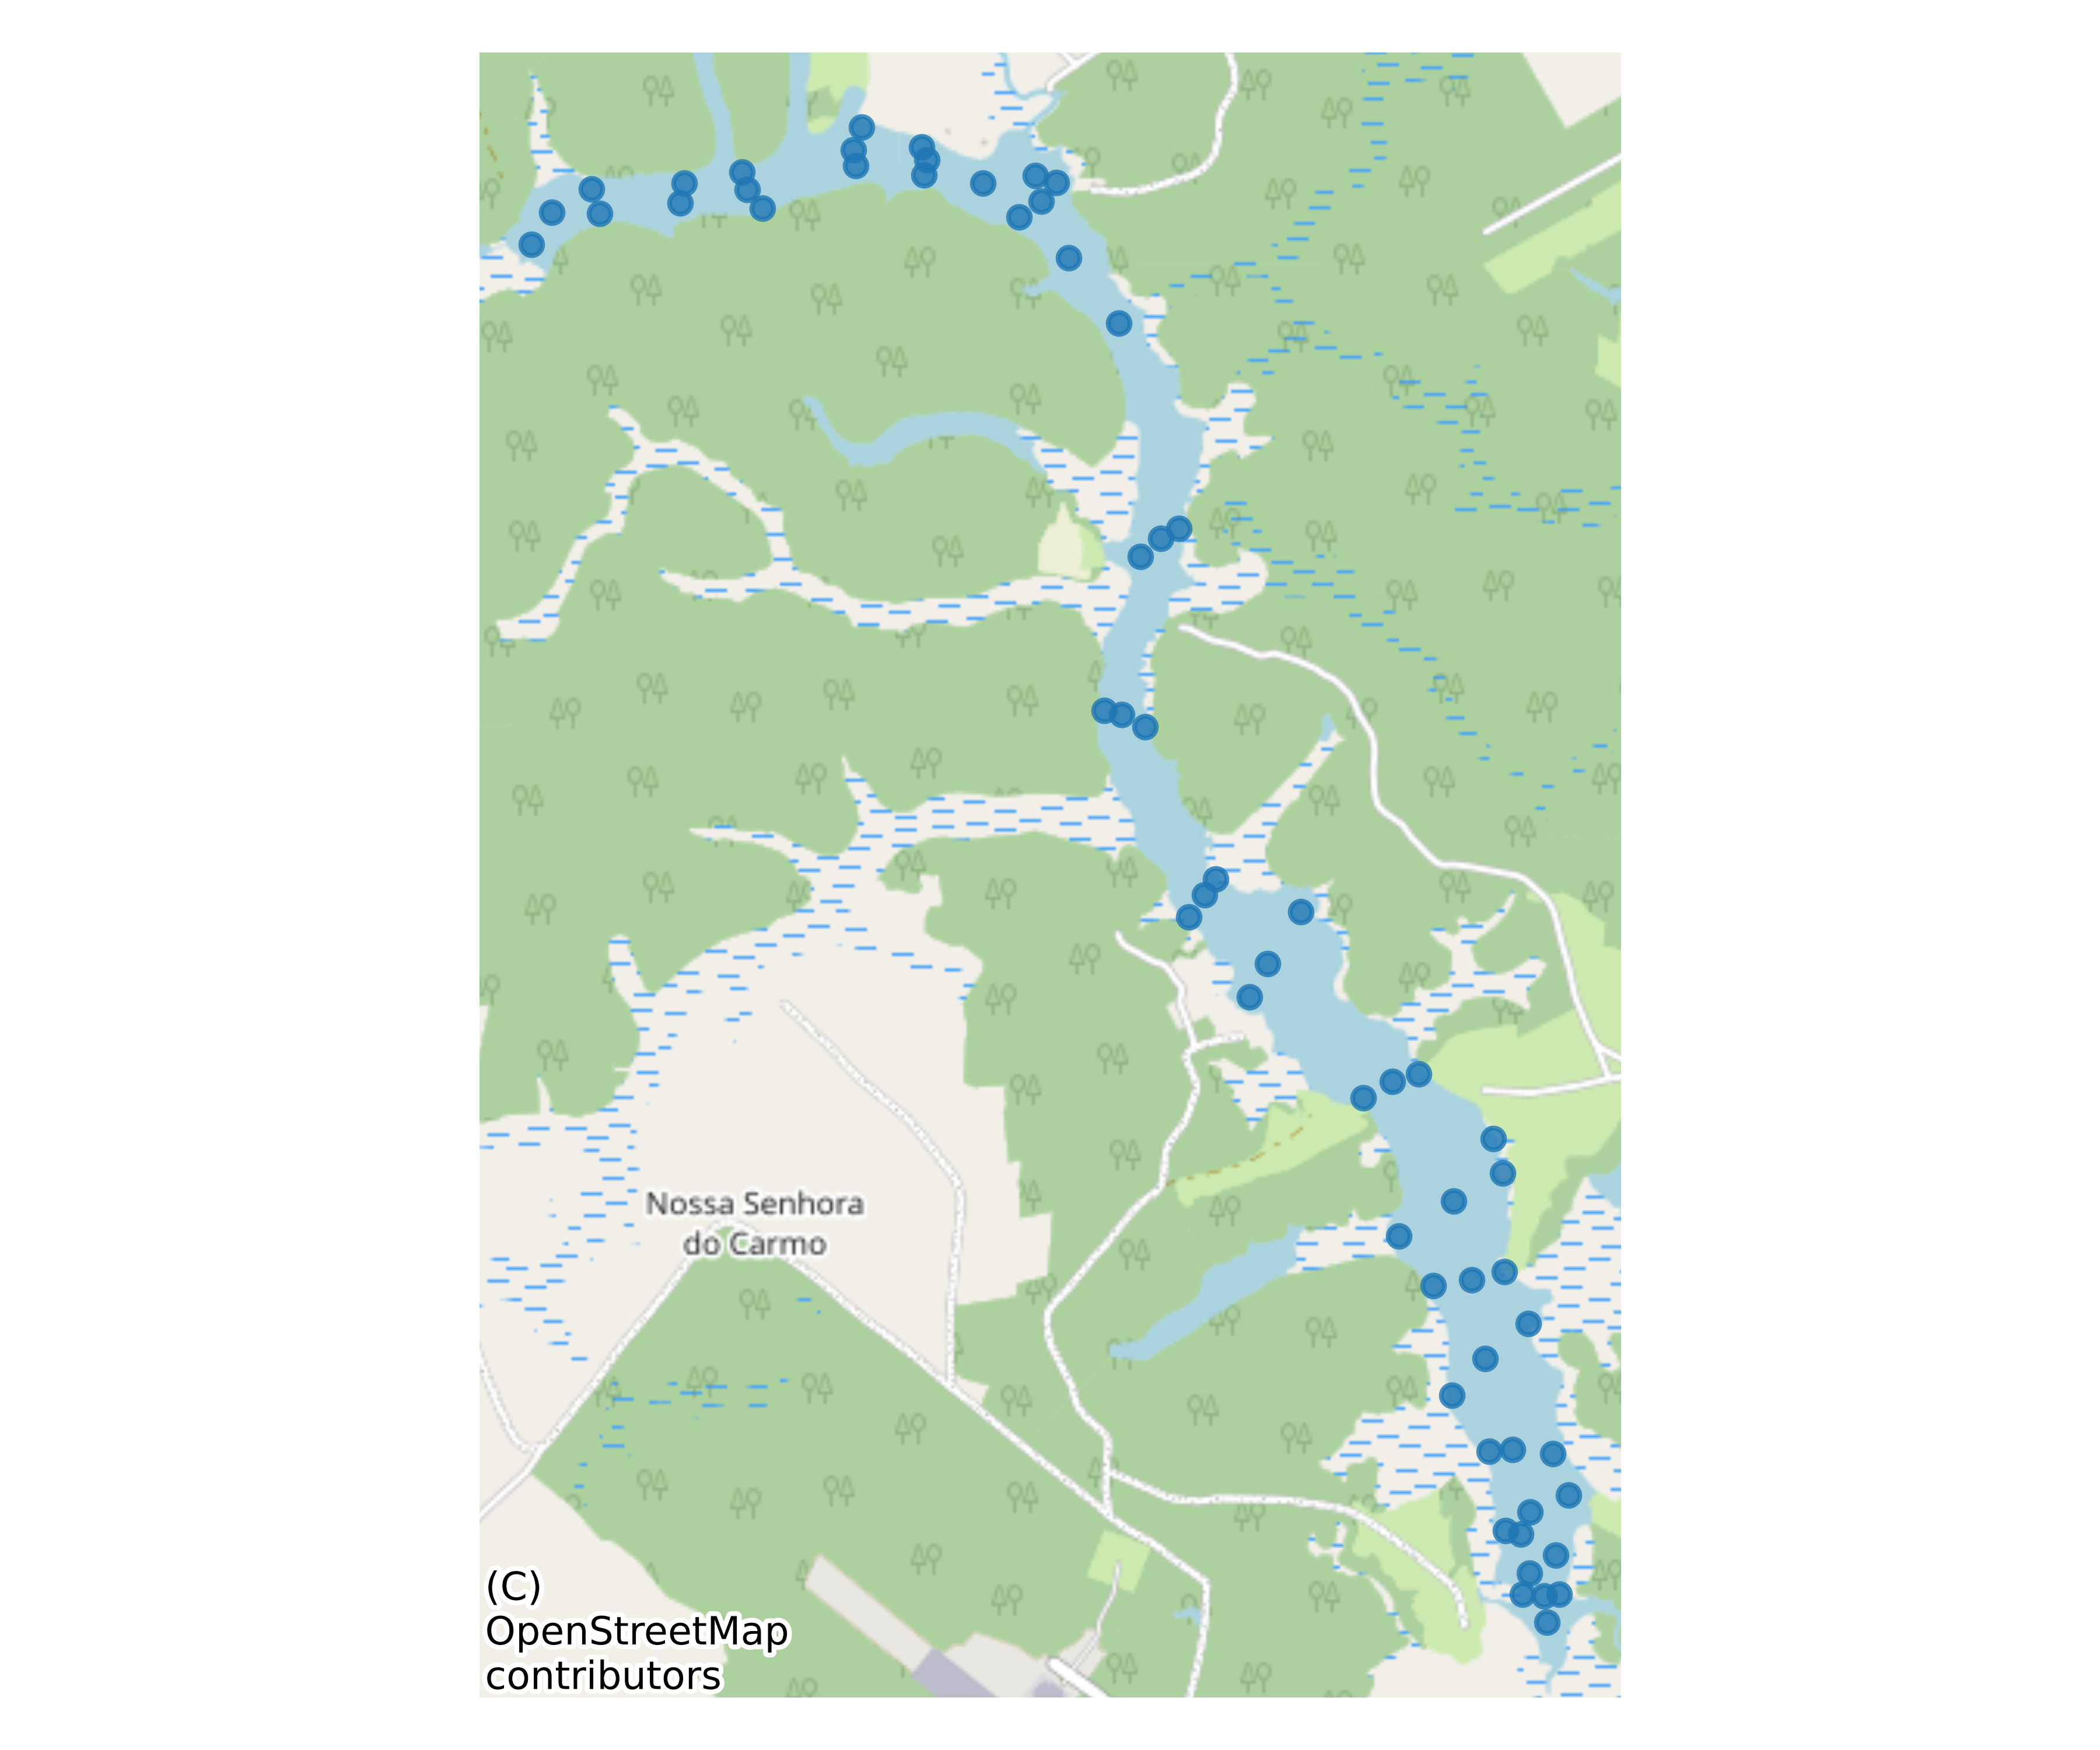
\includegraphics[width=0.75\textwidth]{./figuras/map_points_osm_21S.png}
\caption{Sampling locations in Lago do Serpa (Itacoatiara, AM) on an OpenStreetMap basemap.
Coordinates were converted to latitude/longitude (WGS84, UTM 21S).}
	\label{fig:mapa_pontos}
\end{figure}
\FloatBarrier

Inputs were normalized via z-score using training statistics; multimodal outputs were optionally normalized. The
train/validation/test split used fixed proportions with seed-controlled shuffling. This split (Table~\ref{tab:data_split})
is used in all experiments.

\begin{table}[H]
\centering
\caption{Dataset split.}
\begin{tabular}{lcc}
\toprule
Split & Proportion & Number of samples \\
\midrule
Train & 70\% & 42 \\
Validation & 10\% & 6 \\
Test & 20\% & 12 \\
\bottomrule
\end{tabular}
\label{tab:data_split}
\end{table}




\subsection{Modeling, training, and evaluation}
Normalized inputs were encoded into spike trains using \textit{rate coding}, where firing probability is a
sigmoidal function of the input. The SNN used a dense input layer, a hidden layer with Leaky Integrate-and-Fire
(LIF) neurons, and a linear output layer. Inference runs over $T$ time steps, accumulating hidden activity,
which enables sparse processing; larger $T$ increases temporal resolution but also latency and power consumption.
Training used Adam and MSE with \textit{early stopping} and grid search over $T$, learning rate, threshold,
decay, and hidden size, as well as augmentation noise intensity; the best configuration was selected by the
lowest validation error. For the multimodal model, we used weighted loss and optional target normalization to
predict pH, dissolved oxygen, and turbidity in a single network. From predictions, we defined a composite
pollution index using (i) deviation from neutral pH, (ii) inverse dissolved oxygen, and (iii) normalized
turbidity; CONAMA Resolution 357/2005 is used as a \textbf{normative reference} to interpret estimated levels,
without replacing official indices \cite{conama3572005}. The index was categorized into three relative levels:
low ($[0,0{,}33)$), medium ($[0{,}33,0{,}66)$), and high ($[0{,}66,1]$). Exploratory analyses included boxplots
and correlations, while spatial interpretation used point maps and inverse-distance weighting (IDW) surfaces
for pH, dissolved oxygen, turbidity, and the pollution index. Model comparison used a multiseed benchmark and
a paired sign test on macro metrics, suitable for small samples without normality assumptions.

\subsection{Export and mobile deployment}
After final training, the multimodal model was exported for mobile inference by serializing PyTorch
weights, converting to ONNX while preserving the input/output signature, and transforming to TensorFlow
Lite (TFLite) for a lightweight Android runtime. In the Flutter app, the \textit{.tflite} model and
normalization parameters (mean and standard deviation) are loaded at startup so each sample is normalized
locally before being passed to the TFLite interpreter. Model outputs (pH, dissolved oxygen, turbidity)
are de-normalized and used to compute the composite pollution index in real time. For field operations
without connectivity, the map is shown offline using MBTiles (Mapbox Tiles), preserving spatial context
without internet access.

\subsection{Architecture and integration}
To assess neuromorphic feasibility on constrained hardware, this study focused on implementing and
analyzing SNNs on edge devices. The goal was to evaluate efficiency and accuracy under memory,
processing, and energy constraints typical of edge deployment. The proposed SNN uses Leaky Integrate-and-Fire
(LIF) neurons to optimize sparse event processing. The architecture (Figure~\ref{fig:minhafigura}) organizes
the flow into Input, Processing, and Output stages, exploiting temporal sparsity and activating computation
mainly when relevant changes occur, which favors energy efficiency in autonomous systems.

At the Input stage, Lago do Serpa data are normalized (z-score) and augmented to stabilize training.
The neuromorphic stage performs temporal encoding (\textit{rate coding}) to convert scalar values into
spike trains and runs LIF-based inference. Optimization includes weight and hyperparameter tuning (grid
search and \textit{early stopping}), guided by the loss function. After training, the model is exported
via PyTorch $\rightarrow$ ONNX $\rightarrow$ TFLite for edge deployment. In operation, the same model
runs offline on smartphones, Raspberry Pi, and ESP32, producing multimodal predictions (pH, dissolved
oxygen, turbidity), a pollution index, and spatial maps to support field decision-making.

\begin{figure}[ht!] 
	\centering
	\caption{ 
		Proposed neuromorphic architecture for water-quality prediction, highlighting input
		and preprocessing, neuromorphic training with SNN (LIF) and \textit{rate coding}, the
		PyTorch $\rightarrow$ ONNX $\rightarrow$ TFLite export pipeline, and offline deployment
		on edge devices.
	}
	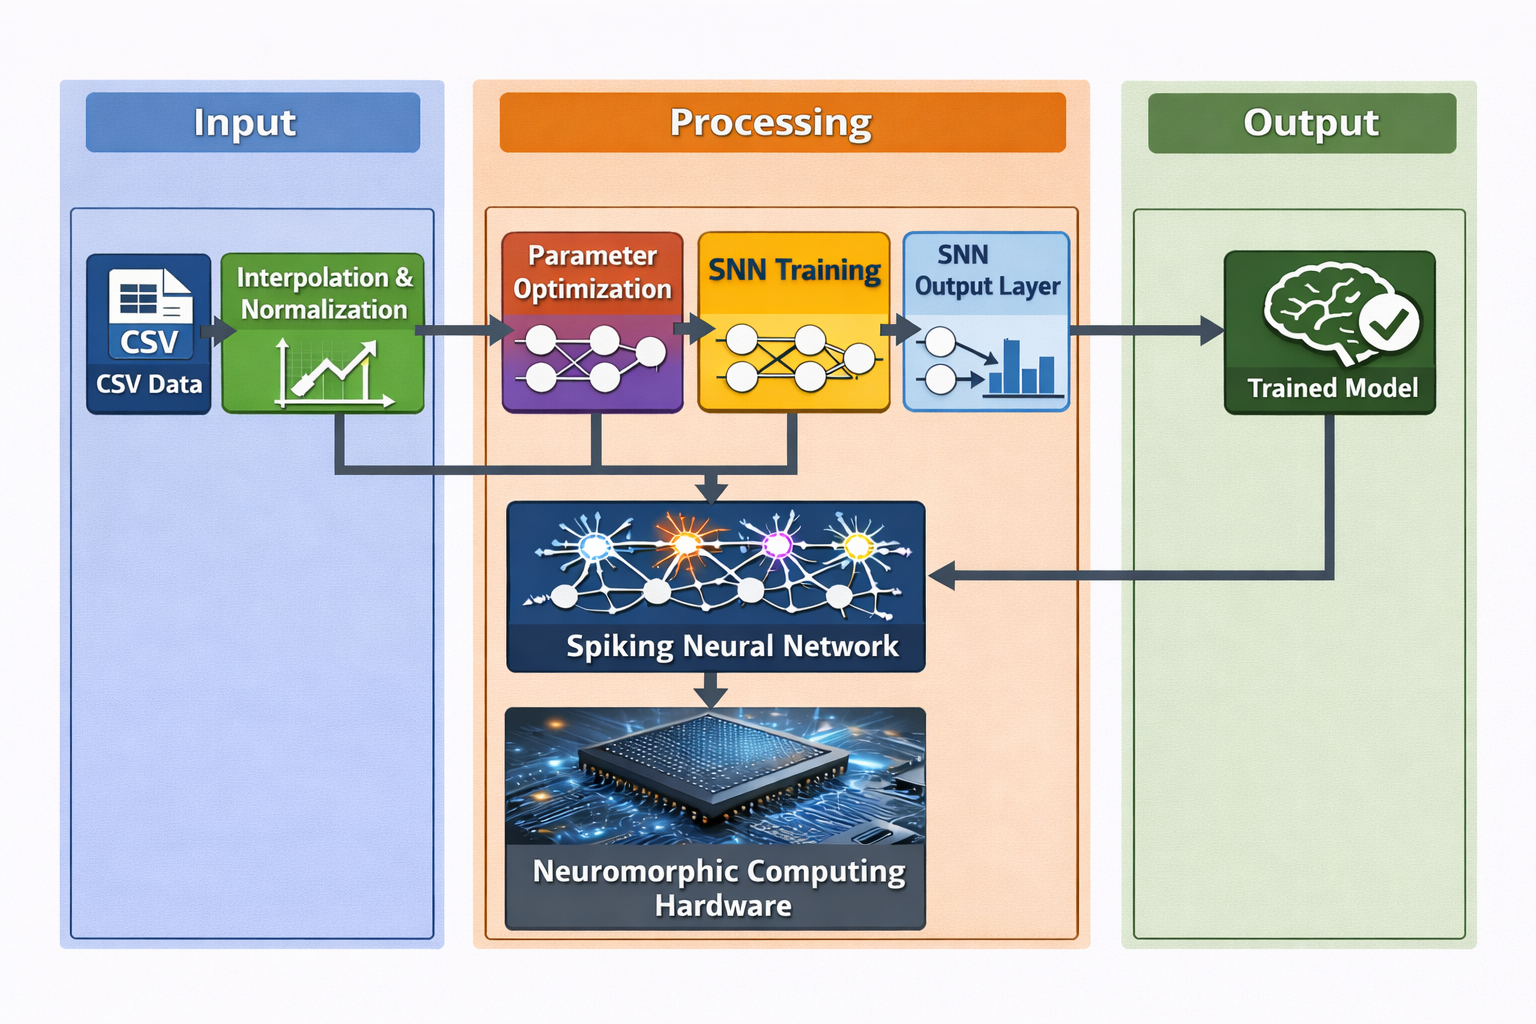
\includegraphics[width=0.8\textwidth]{./figuras/Arquitetura.png}
	\centering
	
	\label{fig:minhafigura}
\end{figure}

\FloatBarrier
\subsection{Hardware specifications for training and inference}

To ensure experimental reproducibility and effective validation, a dedicated workstation was used for
development, offline training, and preliminary inference simulations. Hardware and software specifications
are listed in Table~\ref{tab:hardware}.

\begin{table}[H]
\centering
\caption{Workstation specifications used in the experiments.}
\begin{tabular}{ll}
\toprule
Component & Specification \\
\midrule
CPU & Intel(R) Core(TM) i7-14650HX (24 threads) \\
Memory & 15 GiB \\
GPU & NVIDIA GeForce RTX 4060 (8 GB VRAM), Driver 550.163.01, CUDA 12.4 \\
Operating System & Ubuntu 22.04.5 LTS (64-bit) \\
\bottomrule
\end{tabular}
\label{tab:hardware}
\end{table}

This environment enabled efficient training with surrogate gradients, which are essential to handle
spike non-differentiability prior to portability and optimized deployment on edge devices.

To characterize low-power inference feasibility, the TFLite model was executed on a Raspberry Pi 4B
(ARM64) with the XNNPACK delegate (TFLite kernel optimizer), following the export pipeline described
in Section 3.7. Device specifications are listed in Table~\ref{tab:hardware_rpi}.

\begin{table}[H]
\centering
\caption{Inference device specifications (Raspberry Pi 4B).}
\begin{tabular}{ll}
\toprule
Component & Specification \\
\midrule
Board & Raspberry Pi 4B \\
Architecture & ARM64 \\
Operating System & Linux 6.12.34+rpt-rpi-v8-aarch64 \\
Runtime & TFLite (delegate XNNPACK) \\
\bottomrule
\end{tabular}
\label{tab:hardware_rpi}
\end{table}

Additionally, to evaluate execution on mobile edge devices, the Android app was tested on three phones:
\textit{23021RAAEG} (Qualcomm SoC, Android 15, MemTotal: 5.77 GB), \textit{SM-A566E} (s5e8855 SoC,
Android 16, MemTotal: 7.60 GB), and \textit{2201117SG} (mt6781 SoC, Android 13, MemTotal: 5.86 GB).
These configurations were used for latency benchmarks in the app.

\subsection{Energy measurement}
To quantify incremental energy during inference, an INA219 current sensor was placed in series with
the device power supply and sampled over I\textsuperscript{2}C. Telemetry was recorded periodically
and smoothed with an exponential moving average (EMA), while energy was accumulated over time from the
EMA power estimate. Two windows were considered: \textit{idle} (device idle) and \textit{load}
(inference benchmark). Average power was computed as $P = V \cdot I$, incremental power as
$\Delta P = P_{load} - P_{idle}$, and energy per inference as $\Delta P / \mathrm{throughput}$,
yielding mJ/inf for cross-platform comparison.

\begin{algorithm}[H]
\caption{Energy measurement procedure using the INA219 sensor.}
\begin{algorithmic}[1]
\STATE \textbf{Initialization:}
\STATE Configure INA219 and I\textsuperscript{2}C (calibration 32V/2A).
\STATE Initialize serial communication at 9600 baud.
\STATE Set telemetry period $\Delta t = 500$ ms and EMA coefficient $\alpha = 0.2$.
\STATE \textbf{Real-time sampling:}
\WHILE{running}
\STATE Read bus voltage $V(t)$ and current $I(t)$ from INA219.
\STATE Compute instantaneous power $P(t) = V(t)\cdot I(t)$.
\STATE Update EMA power: $P_{EMA}(t) = \alpha P(t) + (1-\alpha)P_{EMA}(t-1)$.
\STATE Accumulate energy: $E = E + P_{EMA}(t)\cdot \Delta t$.
\STATE Send $(V(t), I(t), P_{EMA}(t), E)$ over serial.
\ENDWHILE
\STATE \textbf{Energy computation (host):}
\STATE Compute mean idle power $\overline{P}_{idle}$ and mean load power $\overline{P}_{load}$.
\STATE Compute $\Delta P = \overline{P}_{load} - \overline{P}_{idle}$ and $E_{inf} = \Delta P / \text{throughput}$.
\end{algorithmic}
\end{algorithm}

For mobile devices, energy was estimated directly in the Android app. Current was obtained via
\textit{BatteryManager} (\texttt{BATTERY\_PROPERTY\_CURRENT\_NOW}) and voltage via
\textit{ACTION\_BATTERY\_CHANGED} (\texttt{EXTRA\_VOLTAGE}), sampled periodically during \textit{idle}
and \textit{load} (benchmark) windows. Power was computed as $P = V \cdot I$ and incremental power as
$\Delta P = P_{load} - P_{idle}$, enabling energy per inference as $\Delta P / \mathrm{throughput}$
from 200 power samples per device.

For the ESP32 (Espressif microcontroller), inference ran in C/C++ (ESP-IDF) with a dedicated benchmark
routine. We performed 10 \textit{warmup runs}, 1000 executions to estimate mean latency and throughput,
and 200 individual samples for standard deviation, as reported in the firmware serial log.

%----------------------------------------------------------------------------------------
%   RESULTADOS
%----------------------------------------------------------------------------------------

\section{RESULTADOS}

Os resultados apresentados a seguir correspondem ao modelo SNN ajustado com
aumento de dados (fator 5, ruído gaussiano leve) e seleção de hiperparâmetros
via busca em grade. As análises exploratórias mostram a distribuição das
variáveis e suas correlações, enquanto as figuras de desempenho destacam a
estabilidade do treinamento e a qualidade das predições em relação aos valores
observados.

Após a busca em grade, a melhor configuração encontrada foi: $hidden\_size=64$,
$time\_steps=15$, $lr=0{,}002$, $\beta=0{,}95$, $thresh=0{,}8$ e ruído de aumento
$\sigma=0{,}02$, com parada antecipada por paciência de 20 épocas. Com essa
configuração, o modelo final atingiu desempenho de teste com $MSE=0{,}0327$ e
$MAE=0{,}1437$ para a predição de pH. Considerando a faixa observada de pH no
conjunto (aprox. 5{,}16 a 6{,}52), o erro médio absoluto representa uma fração
reduzida do intervalo total, indicando boa precisão relativa para um conjunto
de dados pequeno. A Figura~\ref{fig:pred_pH} evidencia a proximidade entre valores
preditos e reais, enquanto a Figura~\ref{fig:hist_loss} mostra convergência
rápida e estável do treinamento.

Também foi treinado um modelo multimodal (multi-saída) para prever simultaneamente
pH, OD e turbidez. O melhor ajuste multimodal apresentou, no conjunto de teste,
as seguintes métricas: $MAE_{pH}=0{,}115$, $MAE_{OD}=0{,}072$ e $MAE_{TURB}=0{,}392$,
com $R^{2}_{pH}=0{,}723$, $R^{2}_{OD}=0{,}908$ e $R^{2}_{TURB}=0{,}909$. Esses valores
indicam bom desempenho para pH e OD, e desempenho aceitável para turbidez. As
Figuras~\ref{fig:multi_pred} e \ref{fig:multi_res} apresentam as predições e
os resíduos do modelo multimodal, respectivamente.

\begin{figure}[ht!]
	\centering
	\begin{minipage}{0.48\textwidth}
		\centering
		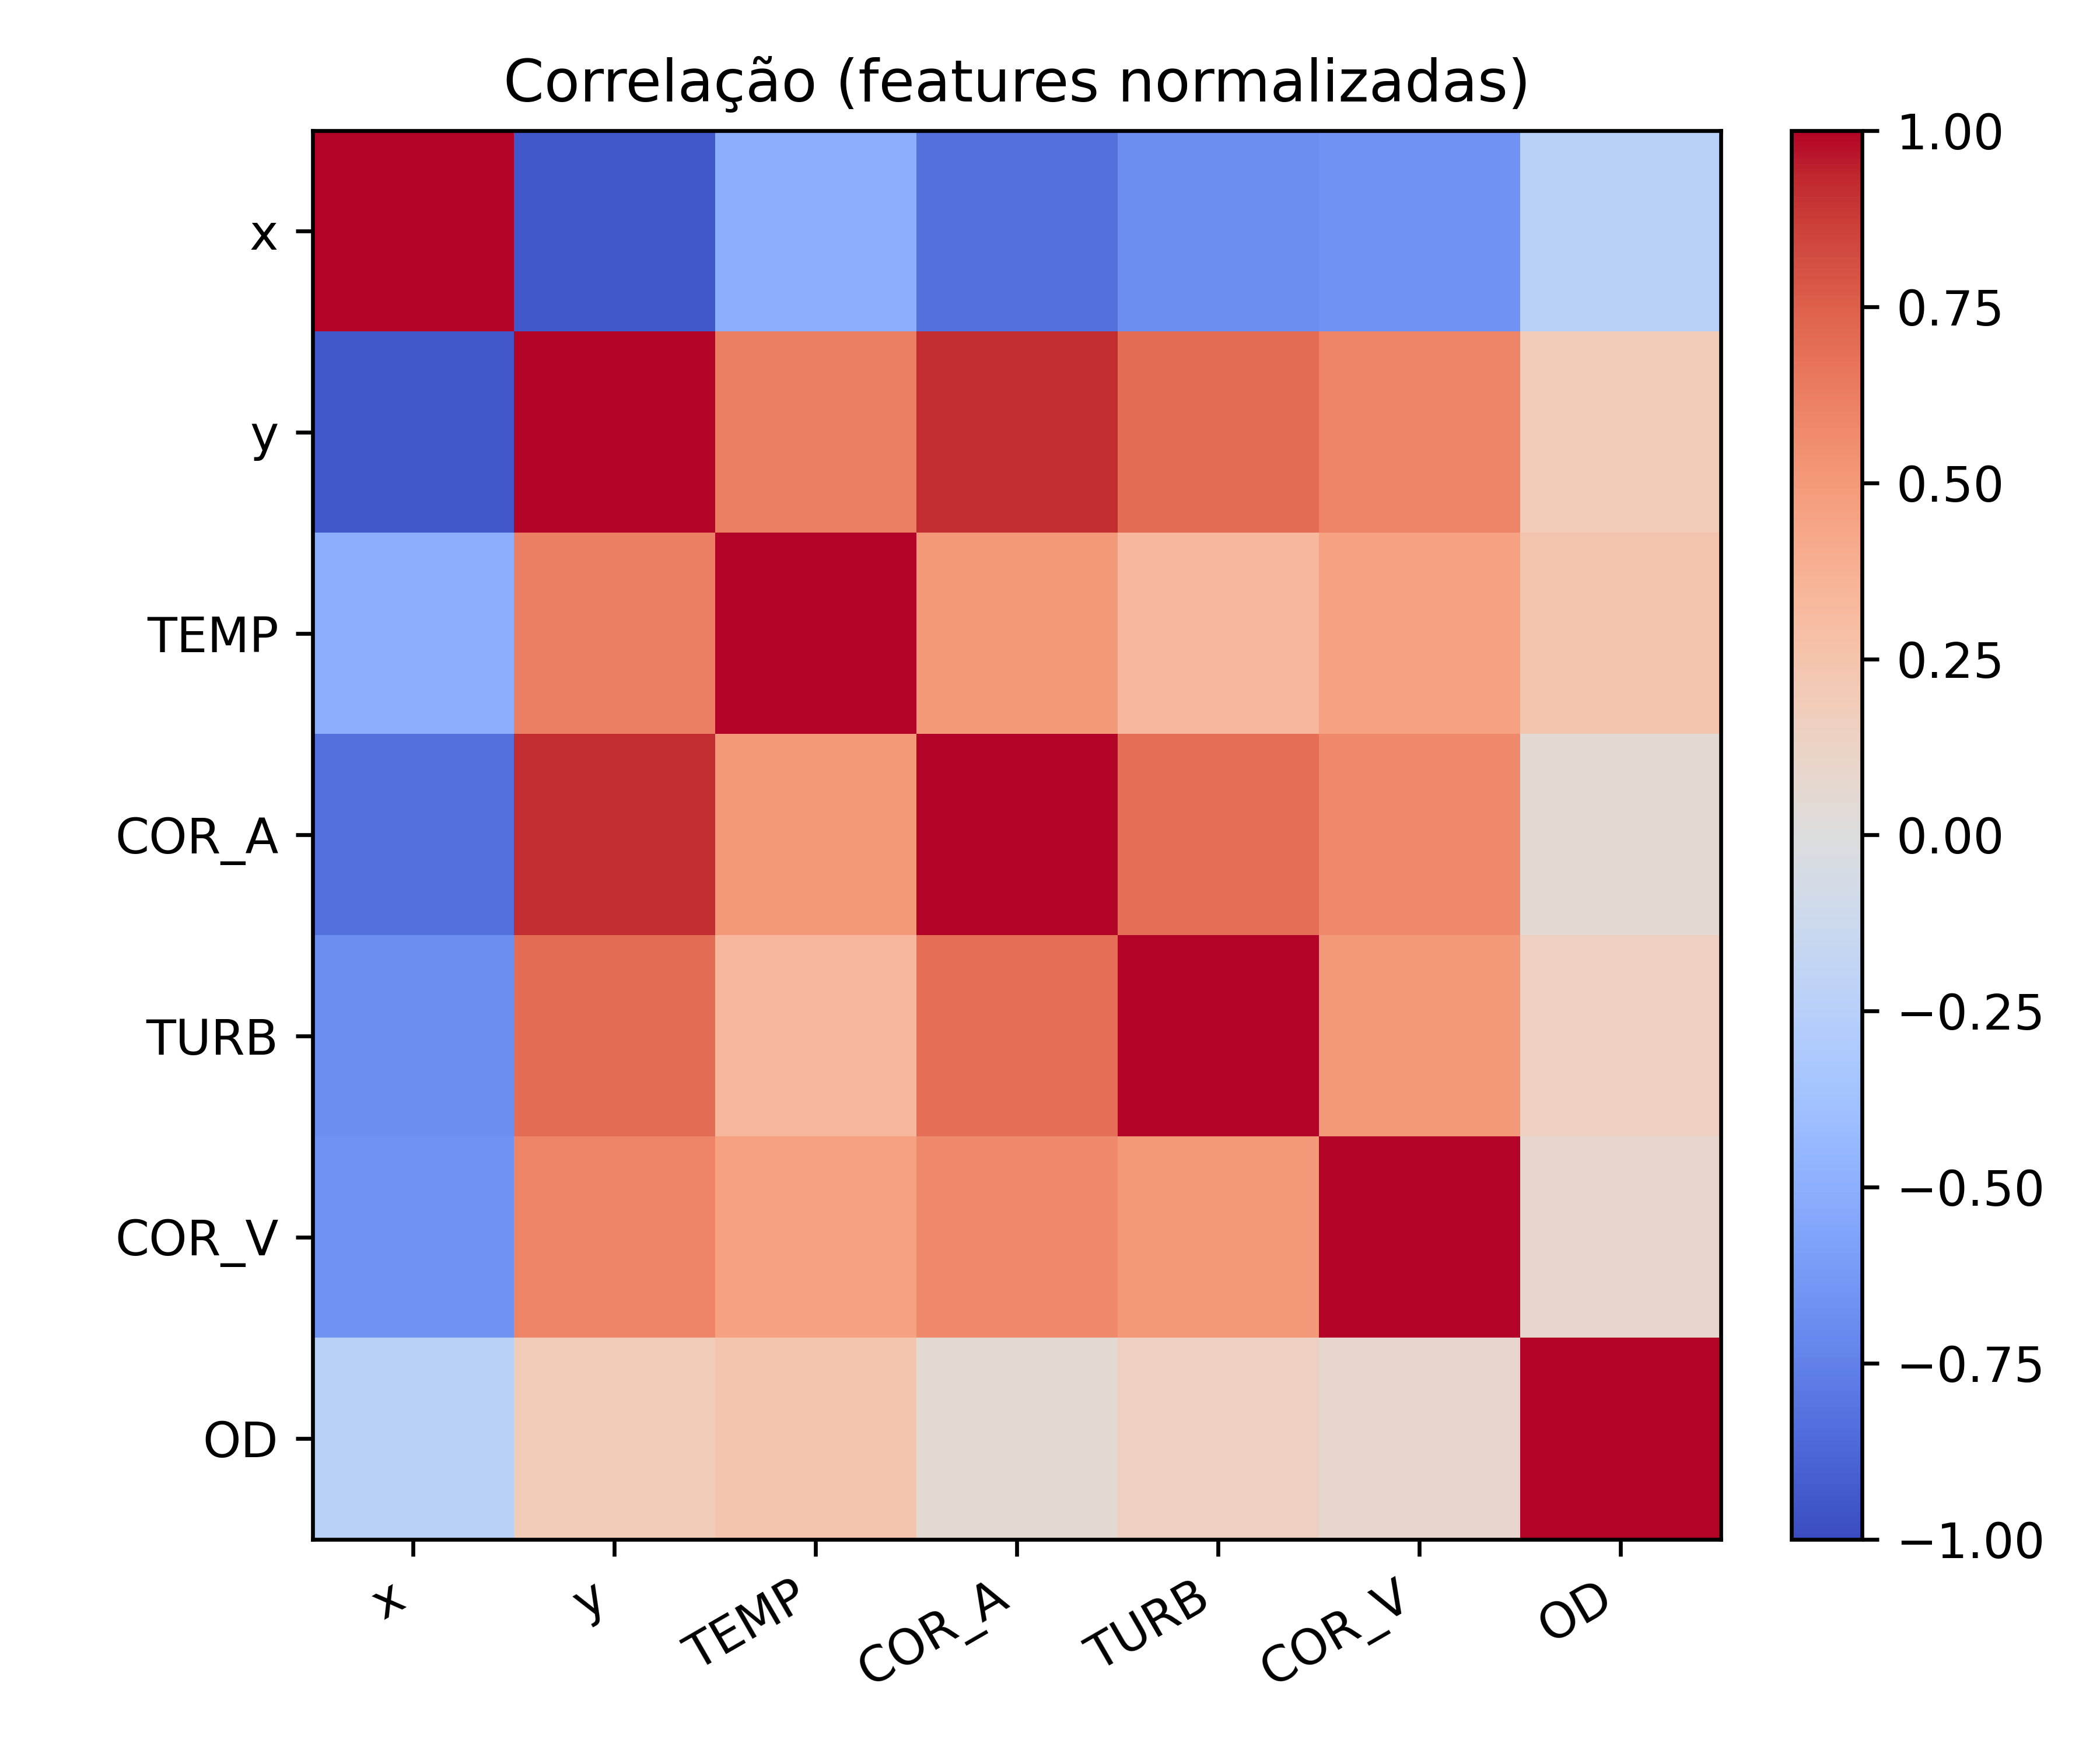
\includegraphics[width=\linewidth]{./figuras/corr_heatmap.png}
		\caption*{(a) Correlação entre variáveis}
	\end{minipage}\hfill
	\begin{minipage}{0.48\textwidth}
		\centering
		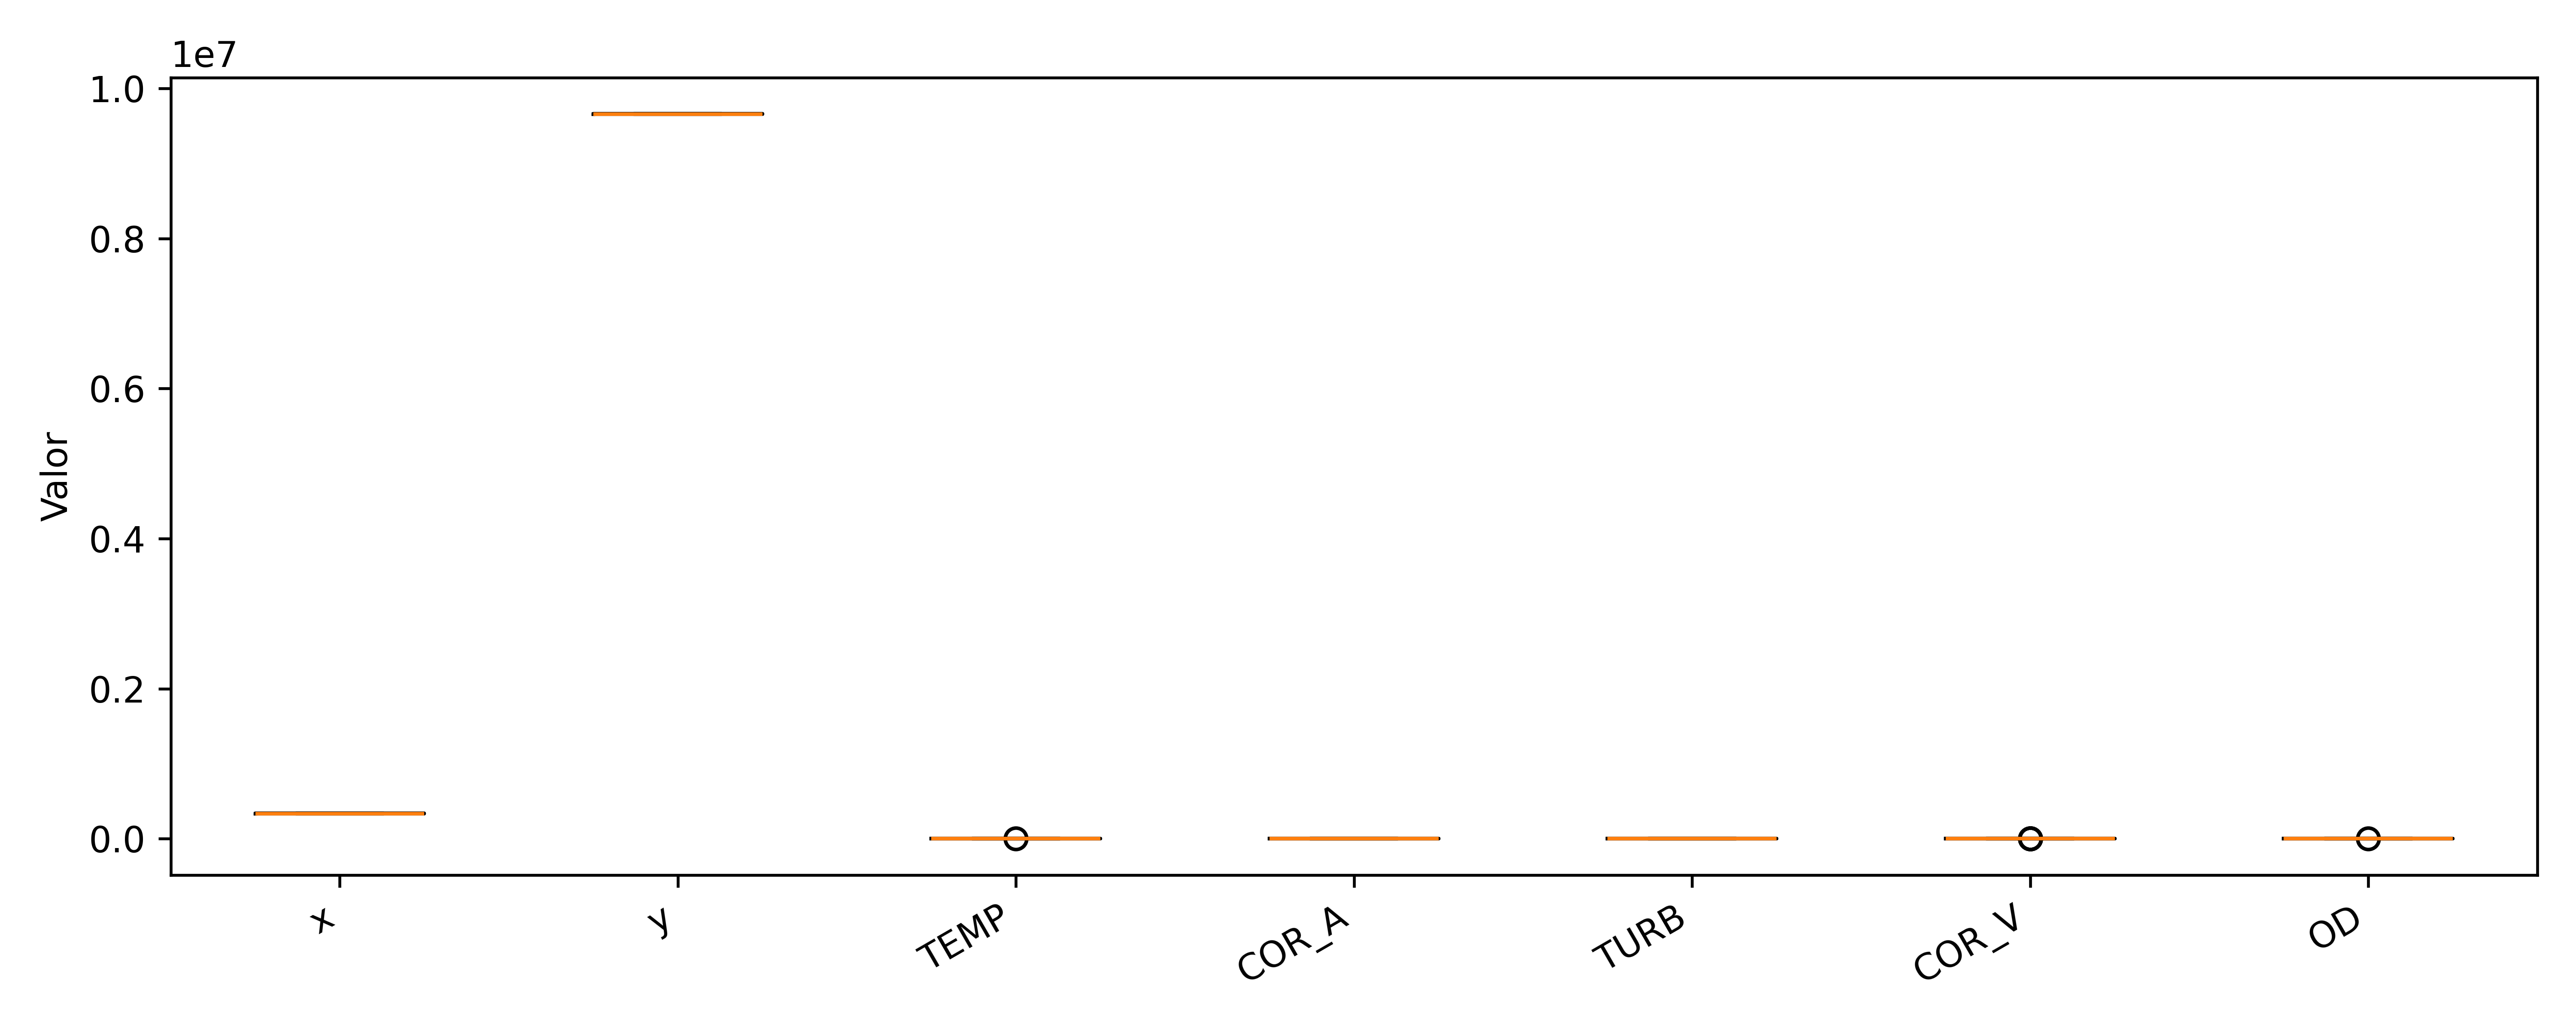
\includegraphics[width=\linewidth]{./figuras/boxplots_features.png}
		\caption*{(b) Boxplots das variáveis}
	\end{minipage}
	\caption{Análise exploratória: correlações e distribuição das variáveis de entrada.}
	\label{fig:exploratoria}
\end{figure}

As Figuras~\ref{fig:exploratoria} e \ref{fig:hist_loss} sintetizam a etapa exploratória. O mapa de
correlação indica relações entre variáveis ambientais, enquanto os boxplots mostram dispersão e
possíveis outliers. Essas informações orientam a interpretação dos modelos e ajudam a contextualizar
as variações observadas nos parâmetros físico-químicos.

\begin{figure}[ht!]
	\centering
	\begin{minipage}{0.48\textwidth}
		\centering
		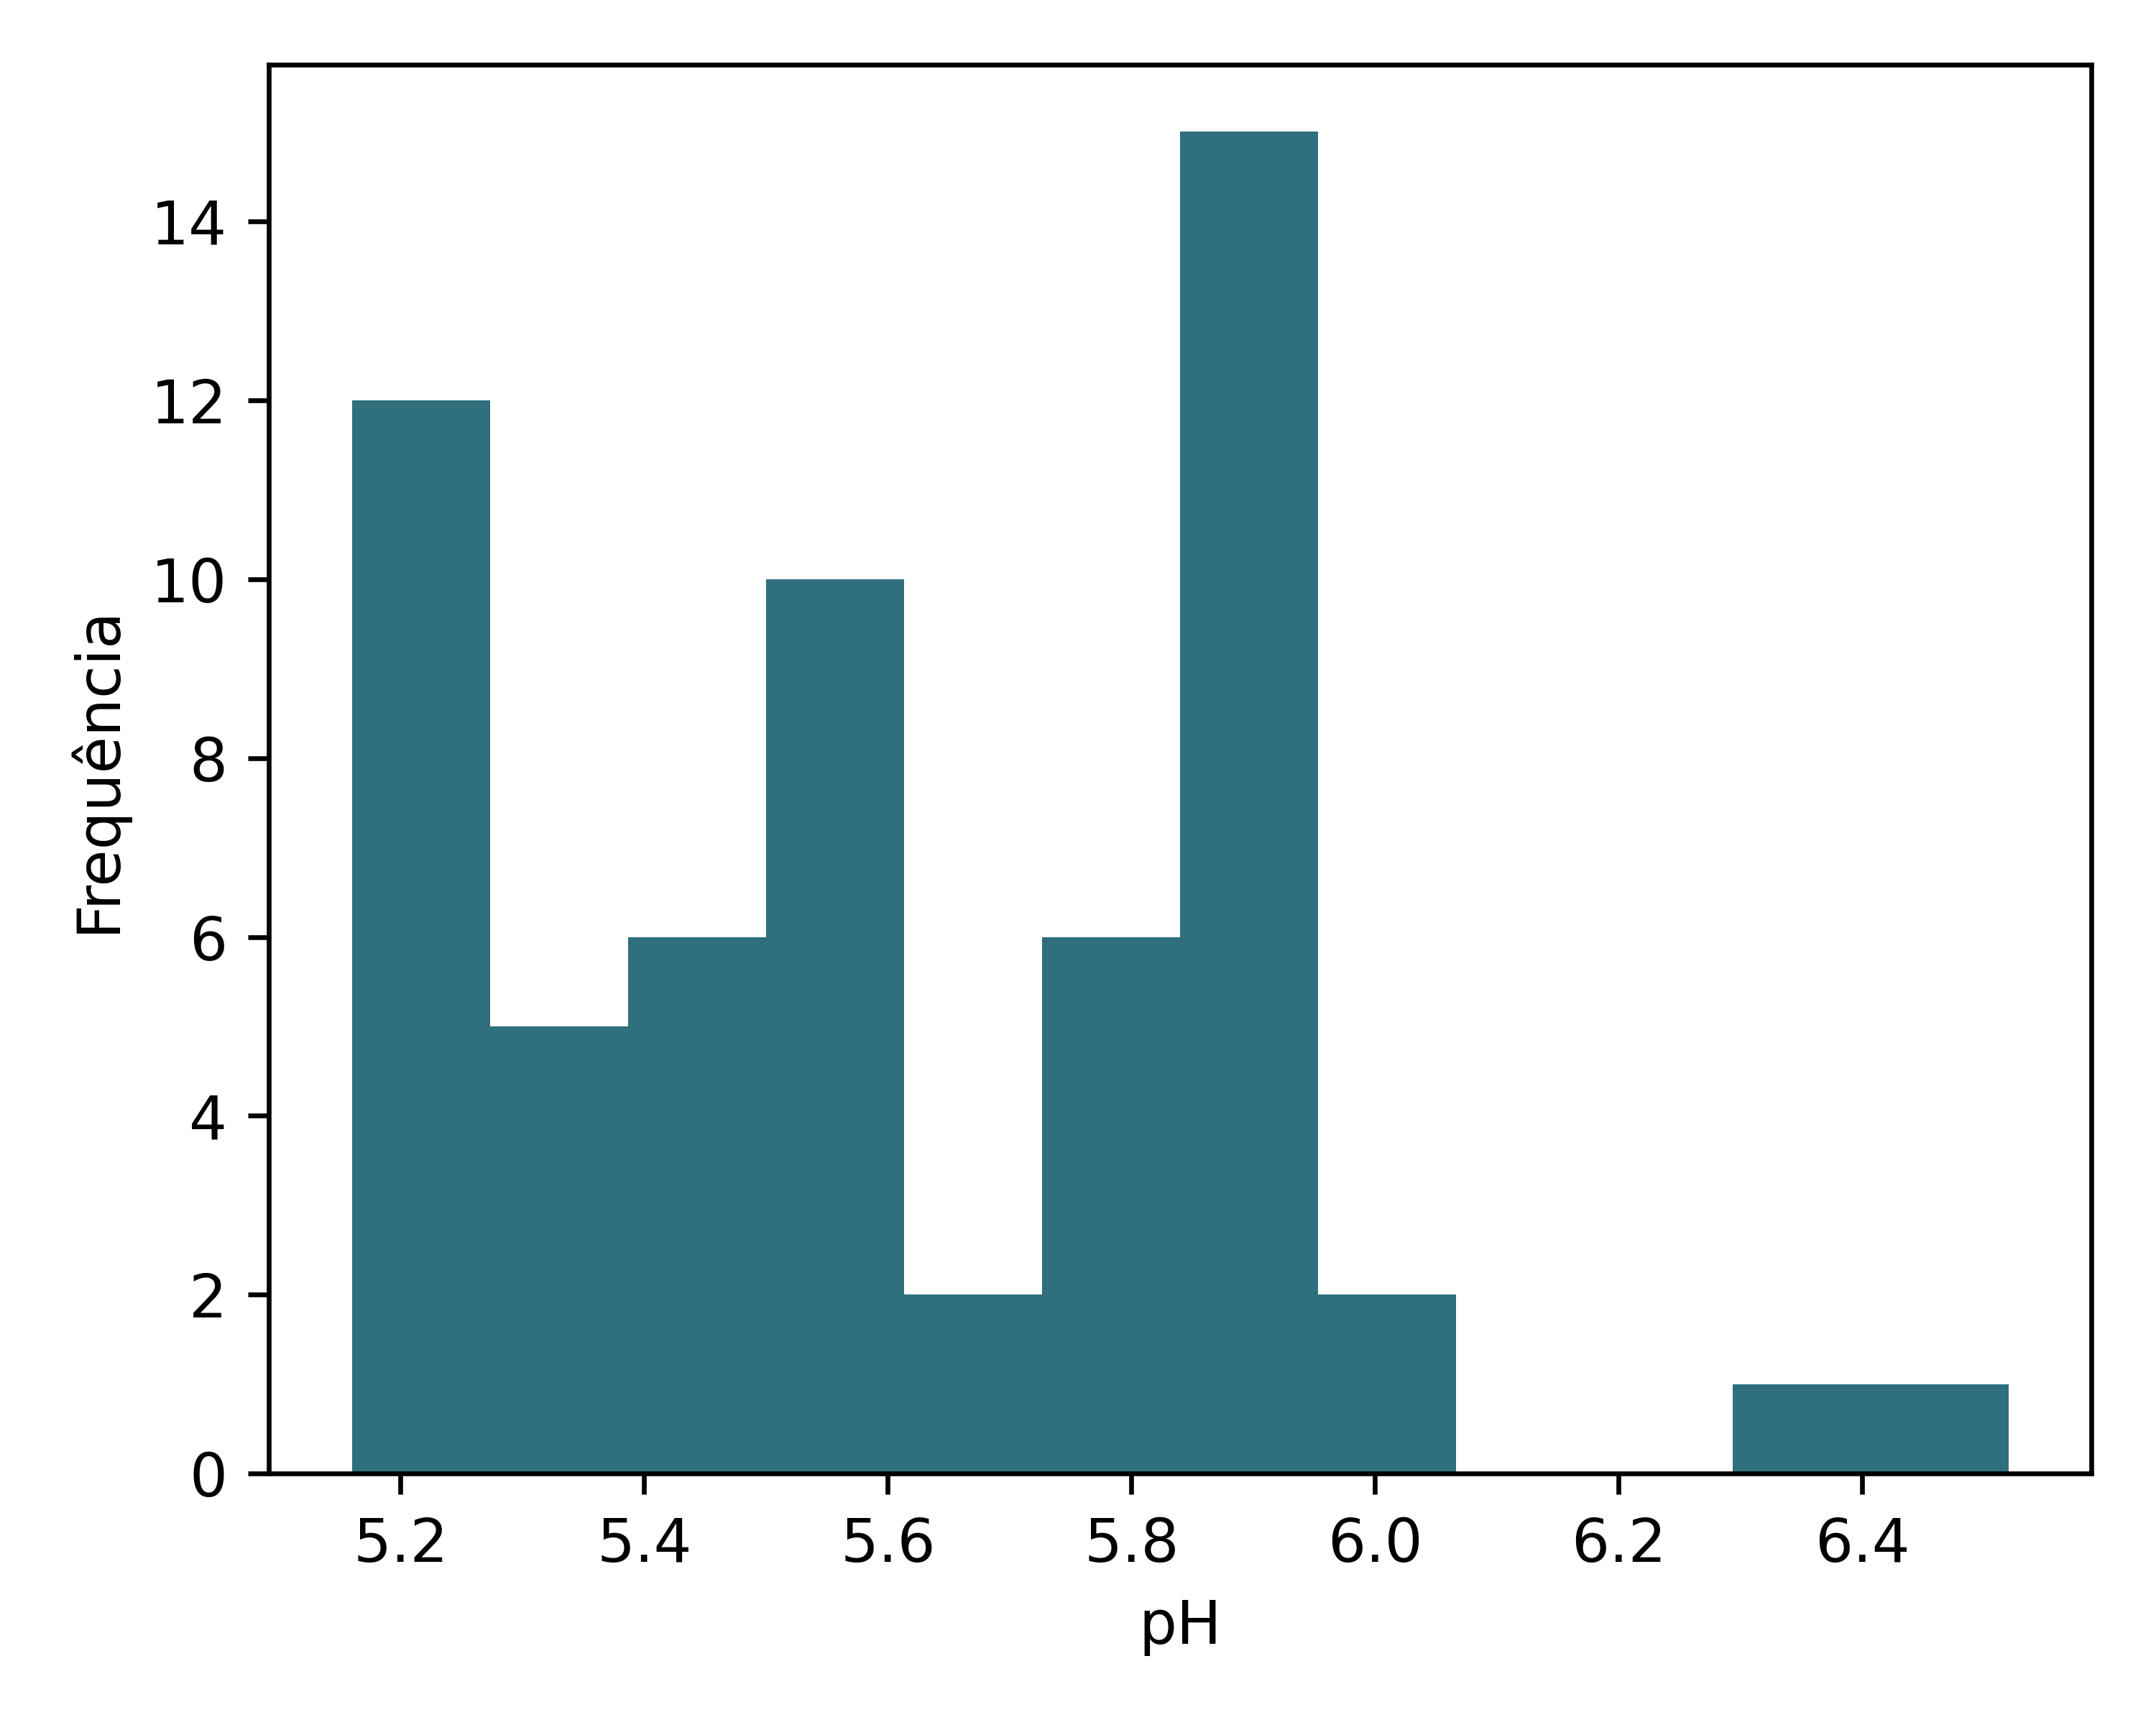
\includegraphics[width=\linewidth]{./figuras/hist_pH.png}
		\caption*{(a) Histograma do pH}
	\end{minipage}\hfill
	\begin{minipage}{0.48\textwidth}
		\centering
		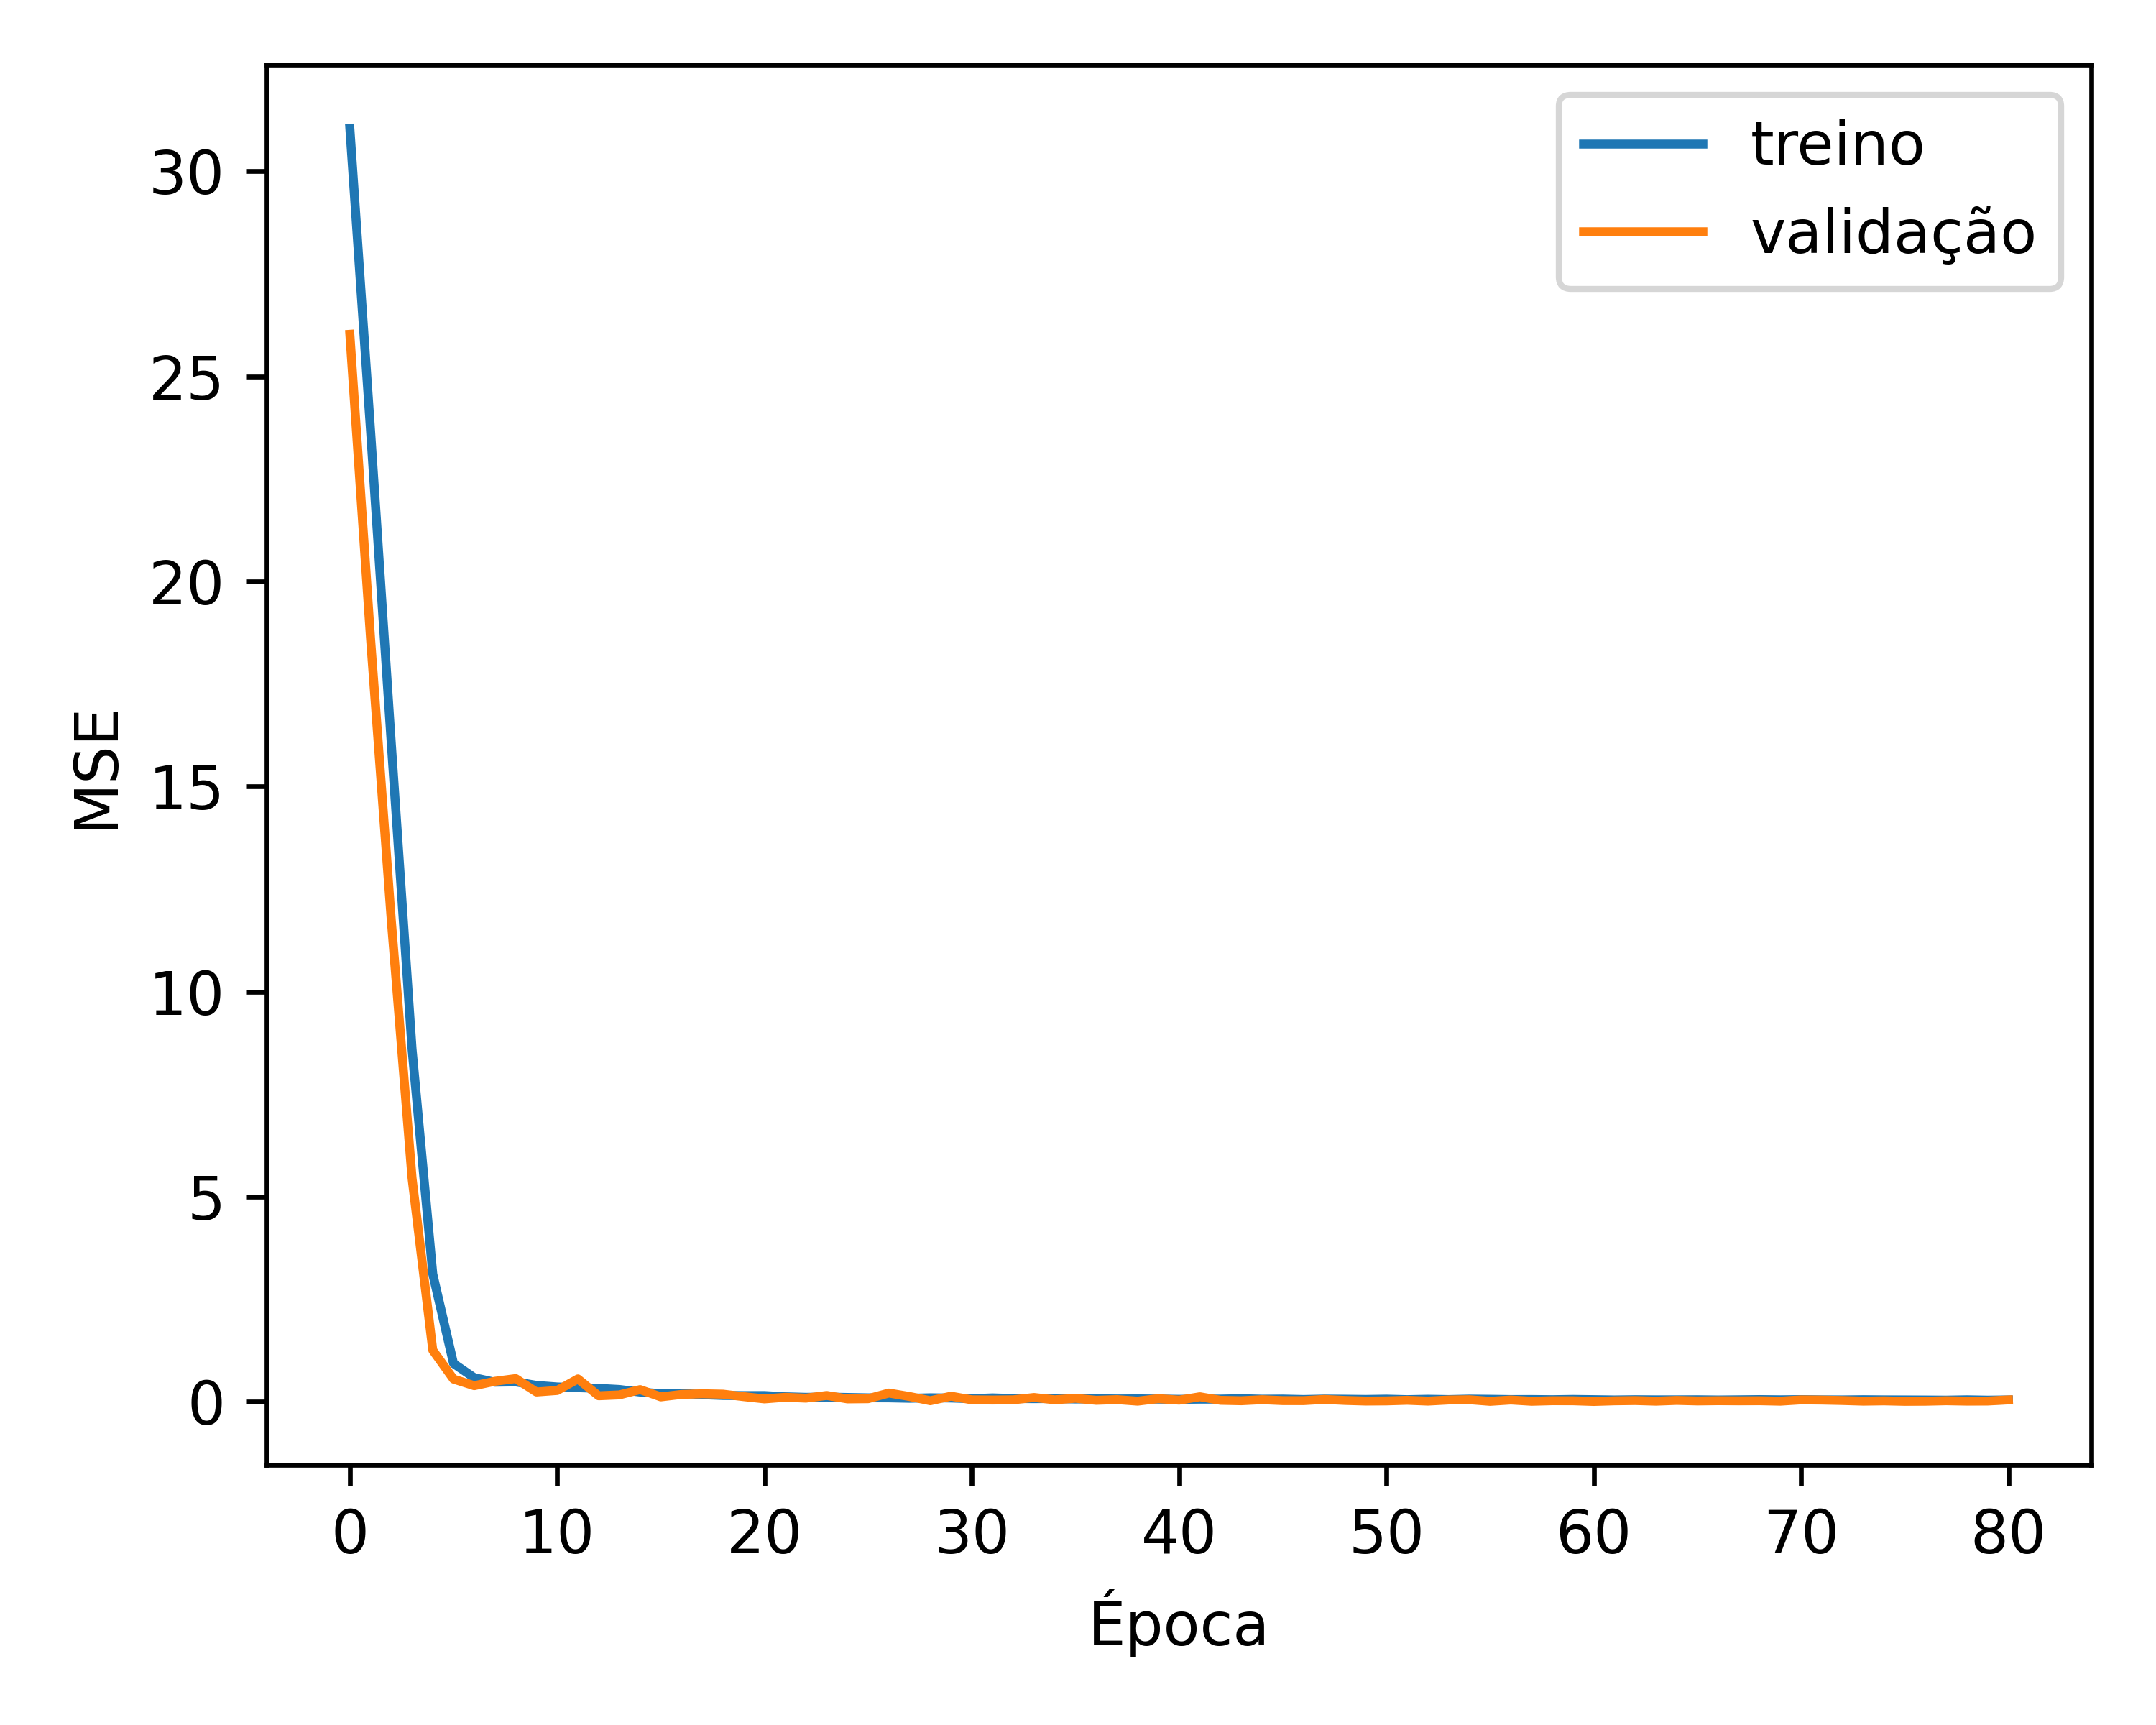
\includegraphics[width=\linewidth]{./figuras/loss_curve.png}
		\caption*{(b) Curva de perda (MSE)}
	\end{minipage}
	\caption{Distribuição do alvo e dinâmica de treinamento/validação.}
	\label{fig:hist_loss}
\end{figure}

O histograma do pH evidencia a concentração de valores em uma faixa estreita, o que reforça a
necessidade de modelos sensíveis a pequenas variações. A curva de perda mostra convergência rápida
e estável, compatível com o uso de \textit{early stopping}.

\begin{figure}[ht!]
	\centering
	\begin{minipage}{0.48\textwidth}
		\centering
		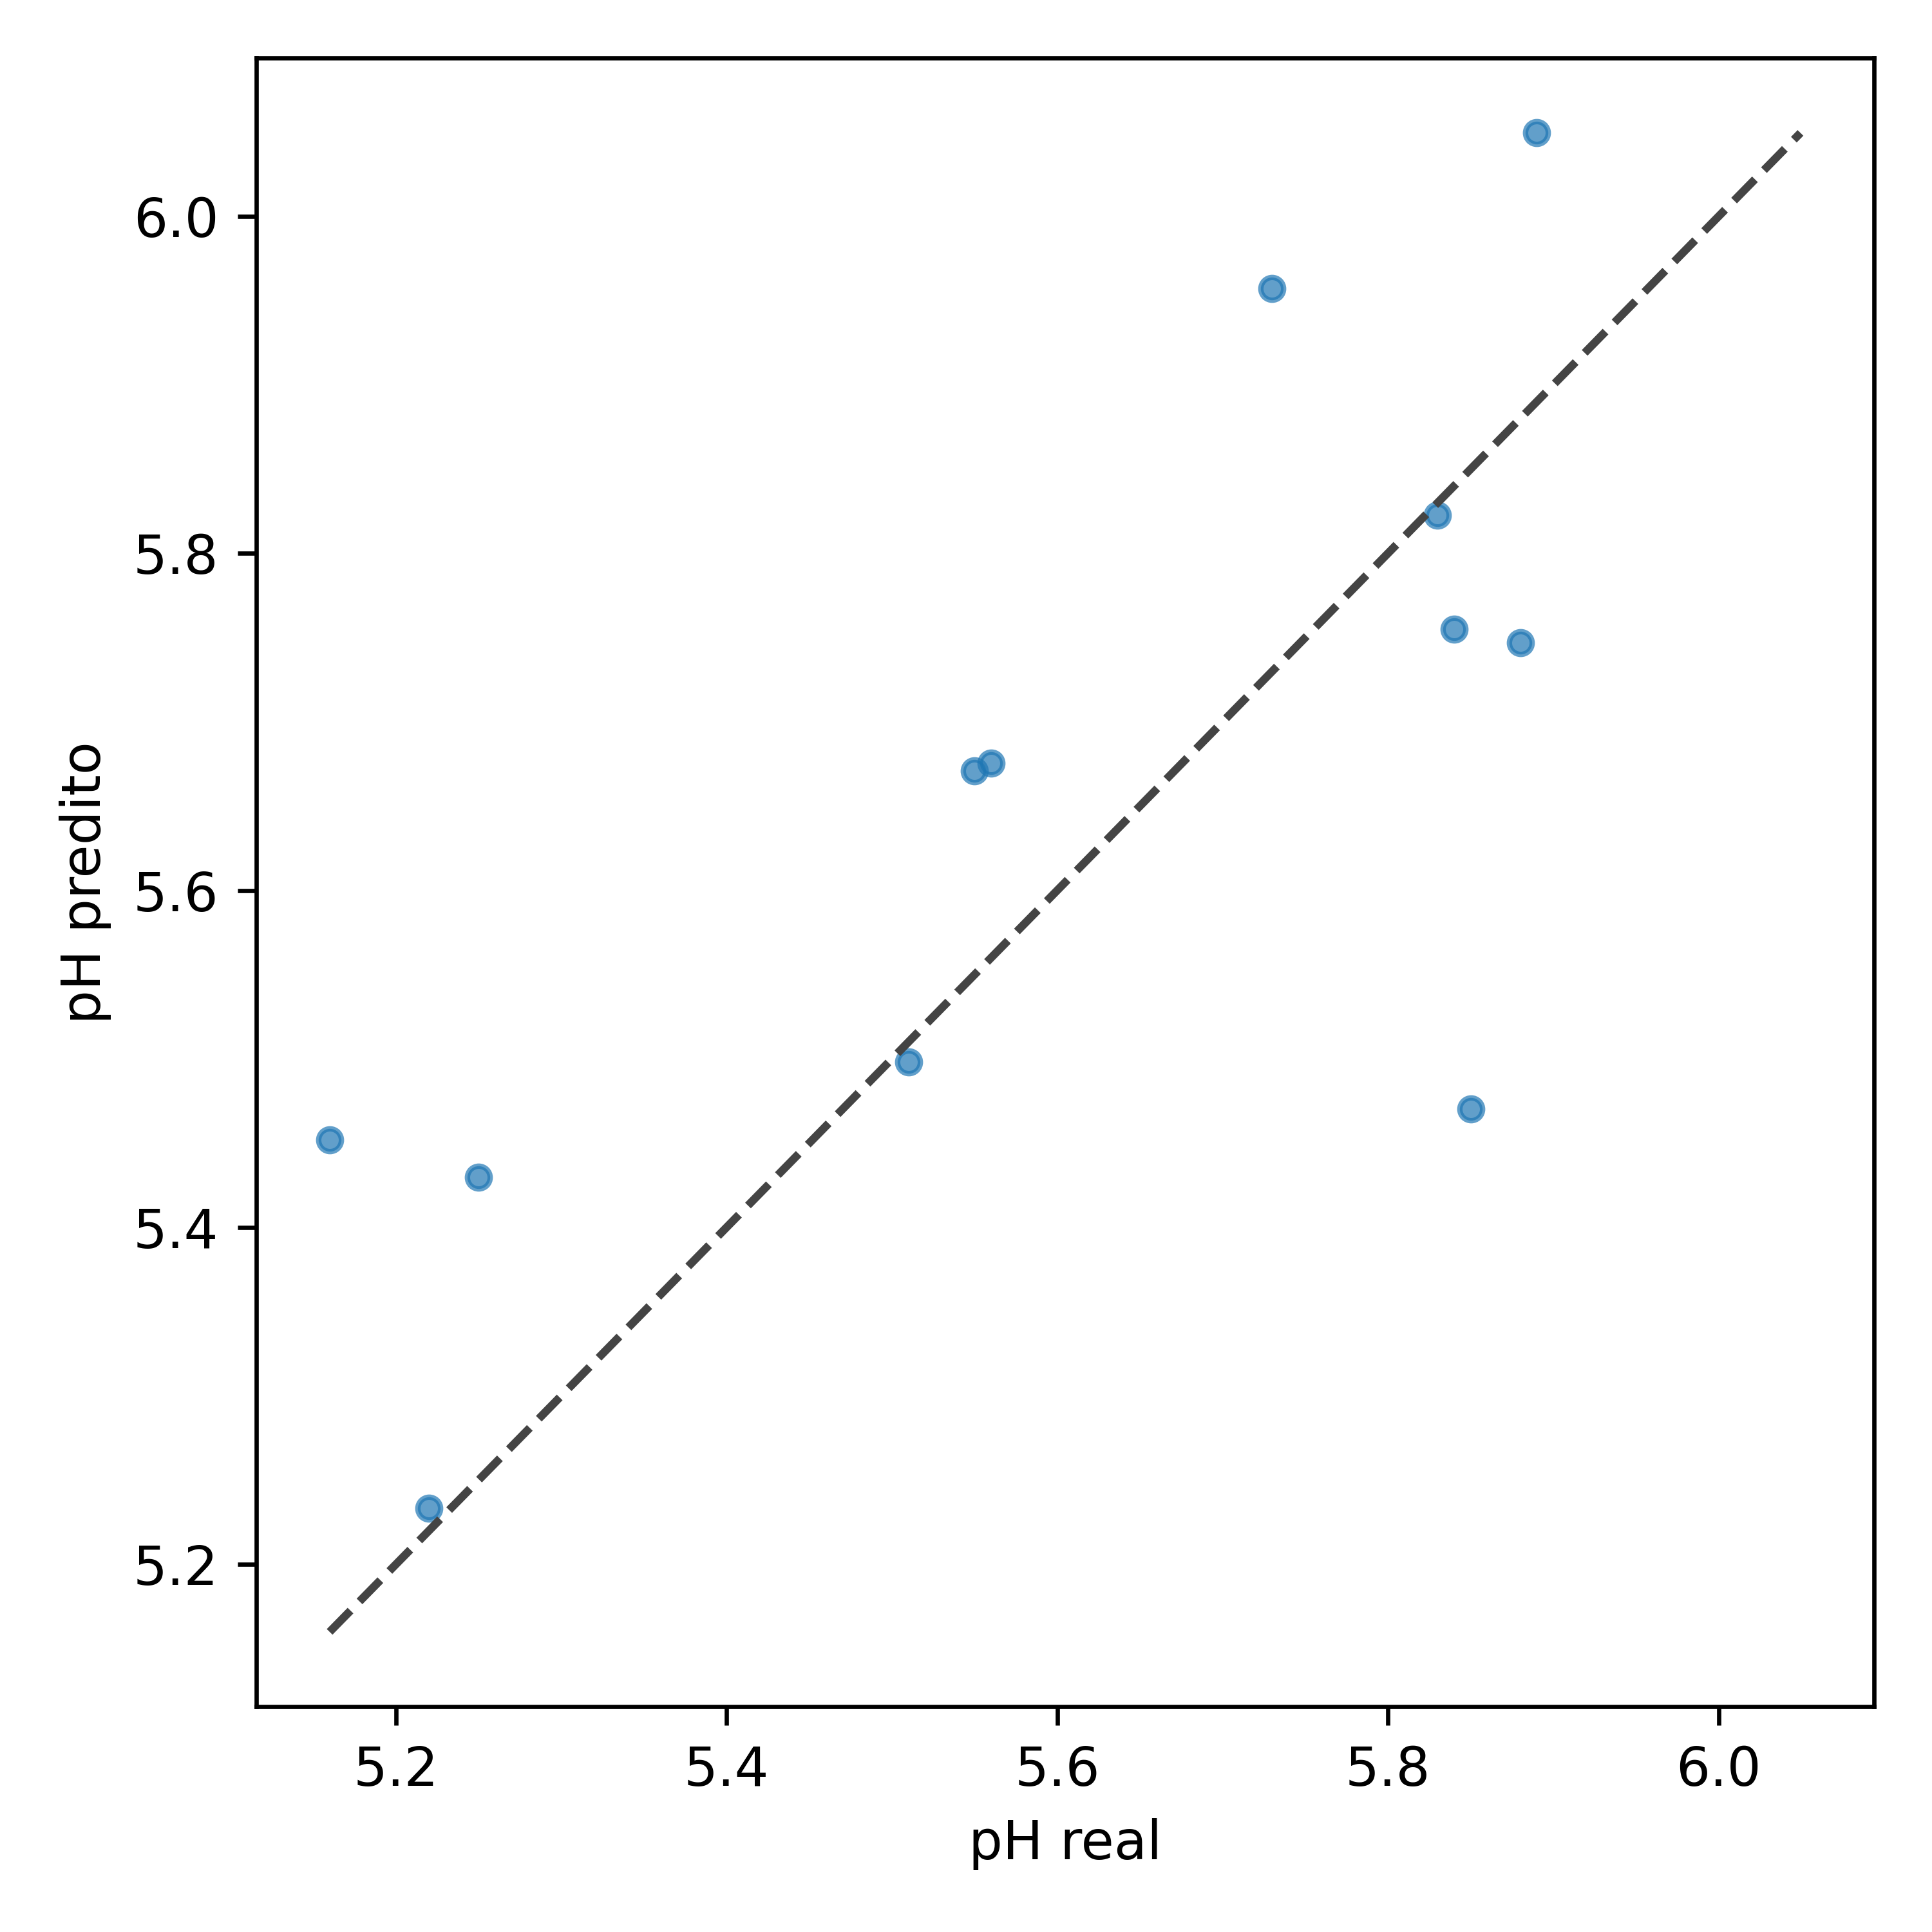
\includegraphics[width=\linewidth]{./figuras/pred_vs_real_pH.png}
		\caption*{(a) Predito vs. real}
	\end{minipage}\hfill
	\begin{minipage}{0.48\textwidth}
		\centering
		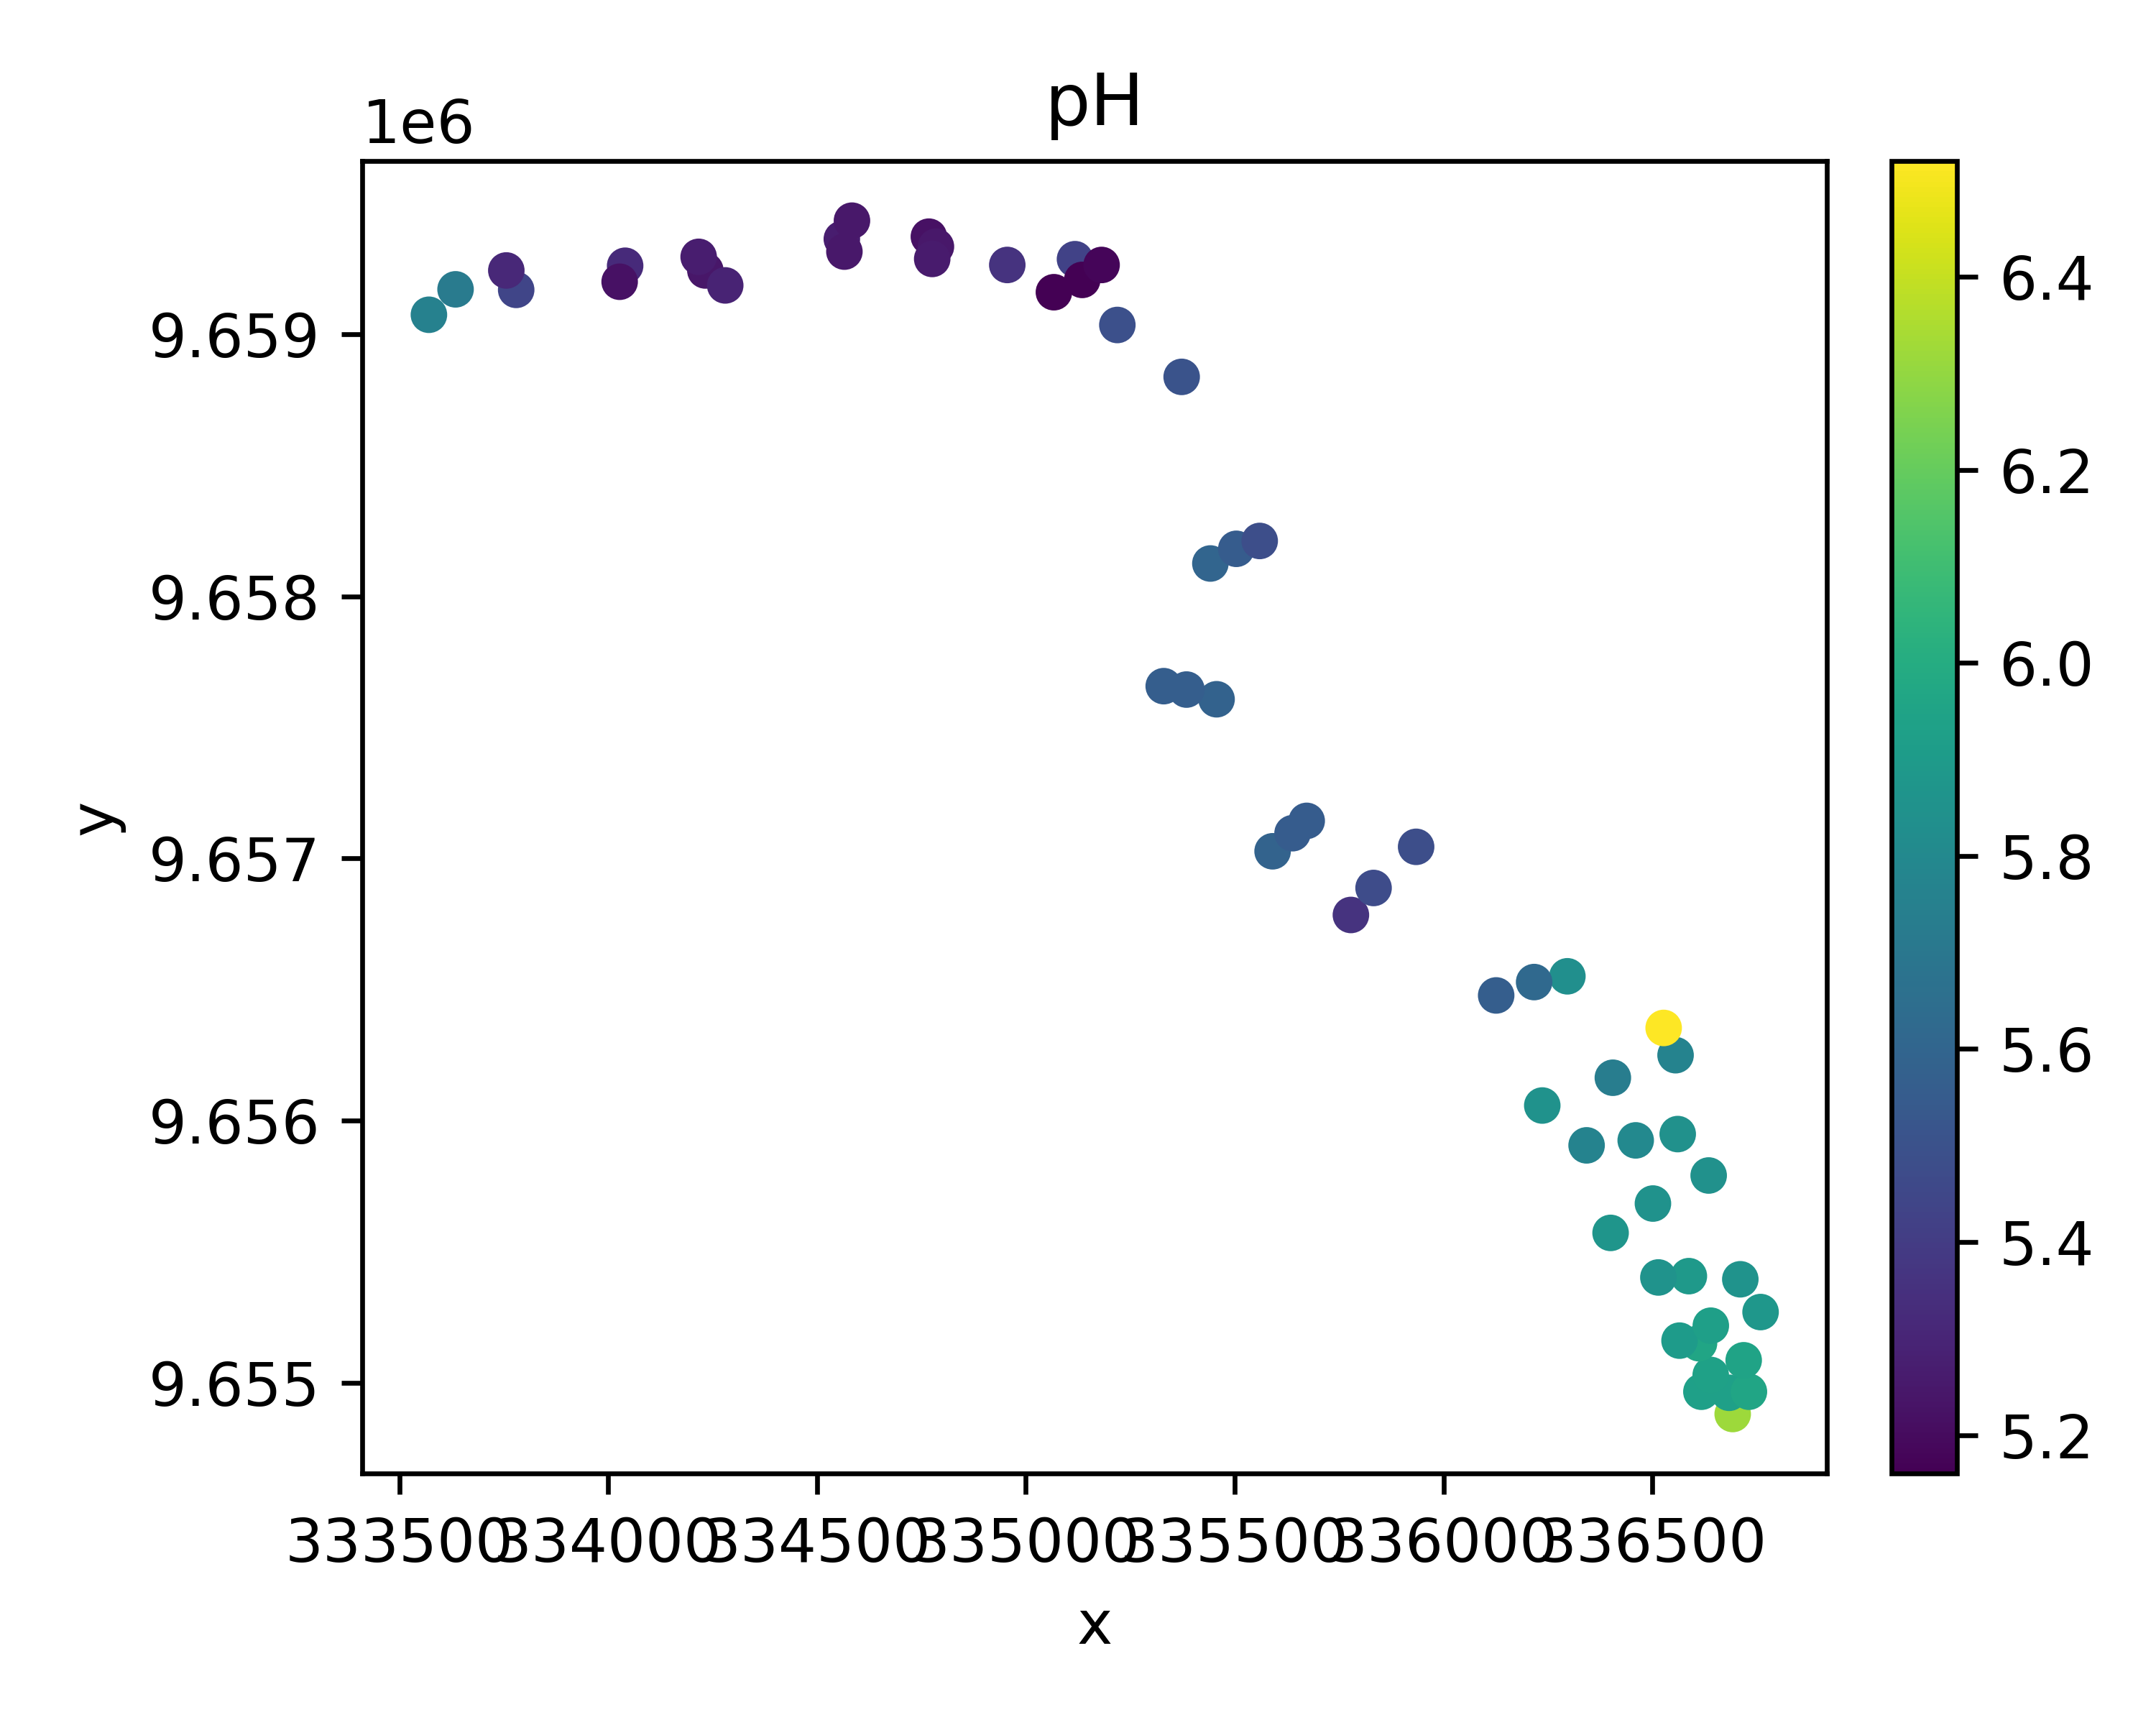
\includegraphics[width=\linewidth]{./figuras/map_pH.png}
		\caption*{(b) Mapa espacial de pH}
	\end{minipage}
	\caption{Desempenho preditivo e padrão espacial do pH no Lago do Serpa.}
	\label{fig:pred_pH}
\end{figure}

Na Figura~\ref{fig:pred_pH}, a proximidade dos pontos à linha de identidade indica boa capacidade
do modelo em reproduzir o pH observado. O mapa espacial do pH revela gradientes coerentes no lago,
com regiões de valores mais elevados concentradas em setores específicos.

\begin{figure}[ht!]
	\centering
	\begin{minipage}{0.48\textwidth}
		\centering
		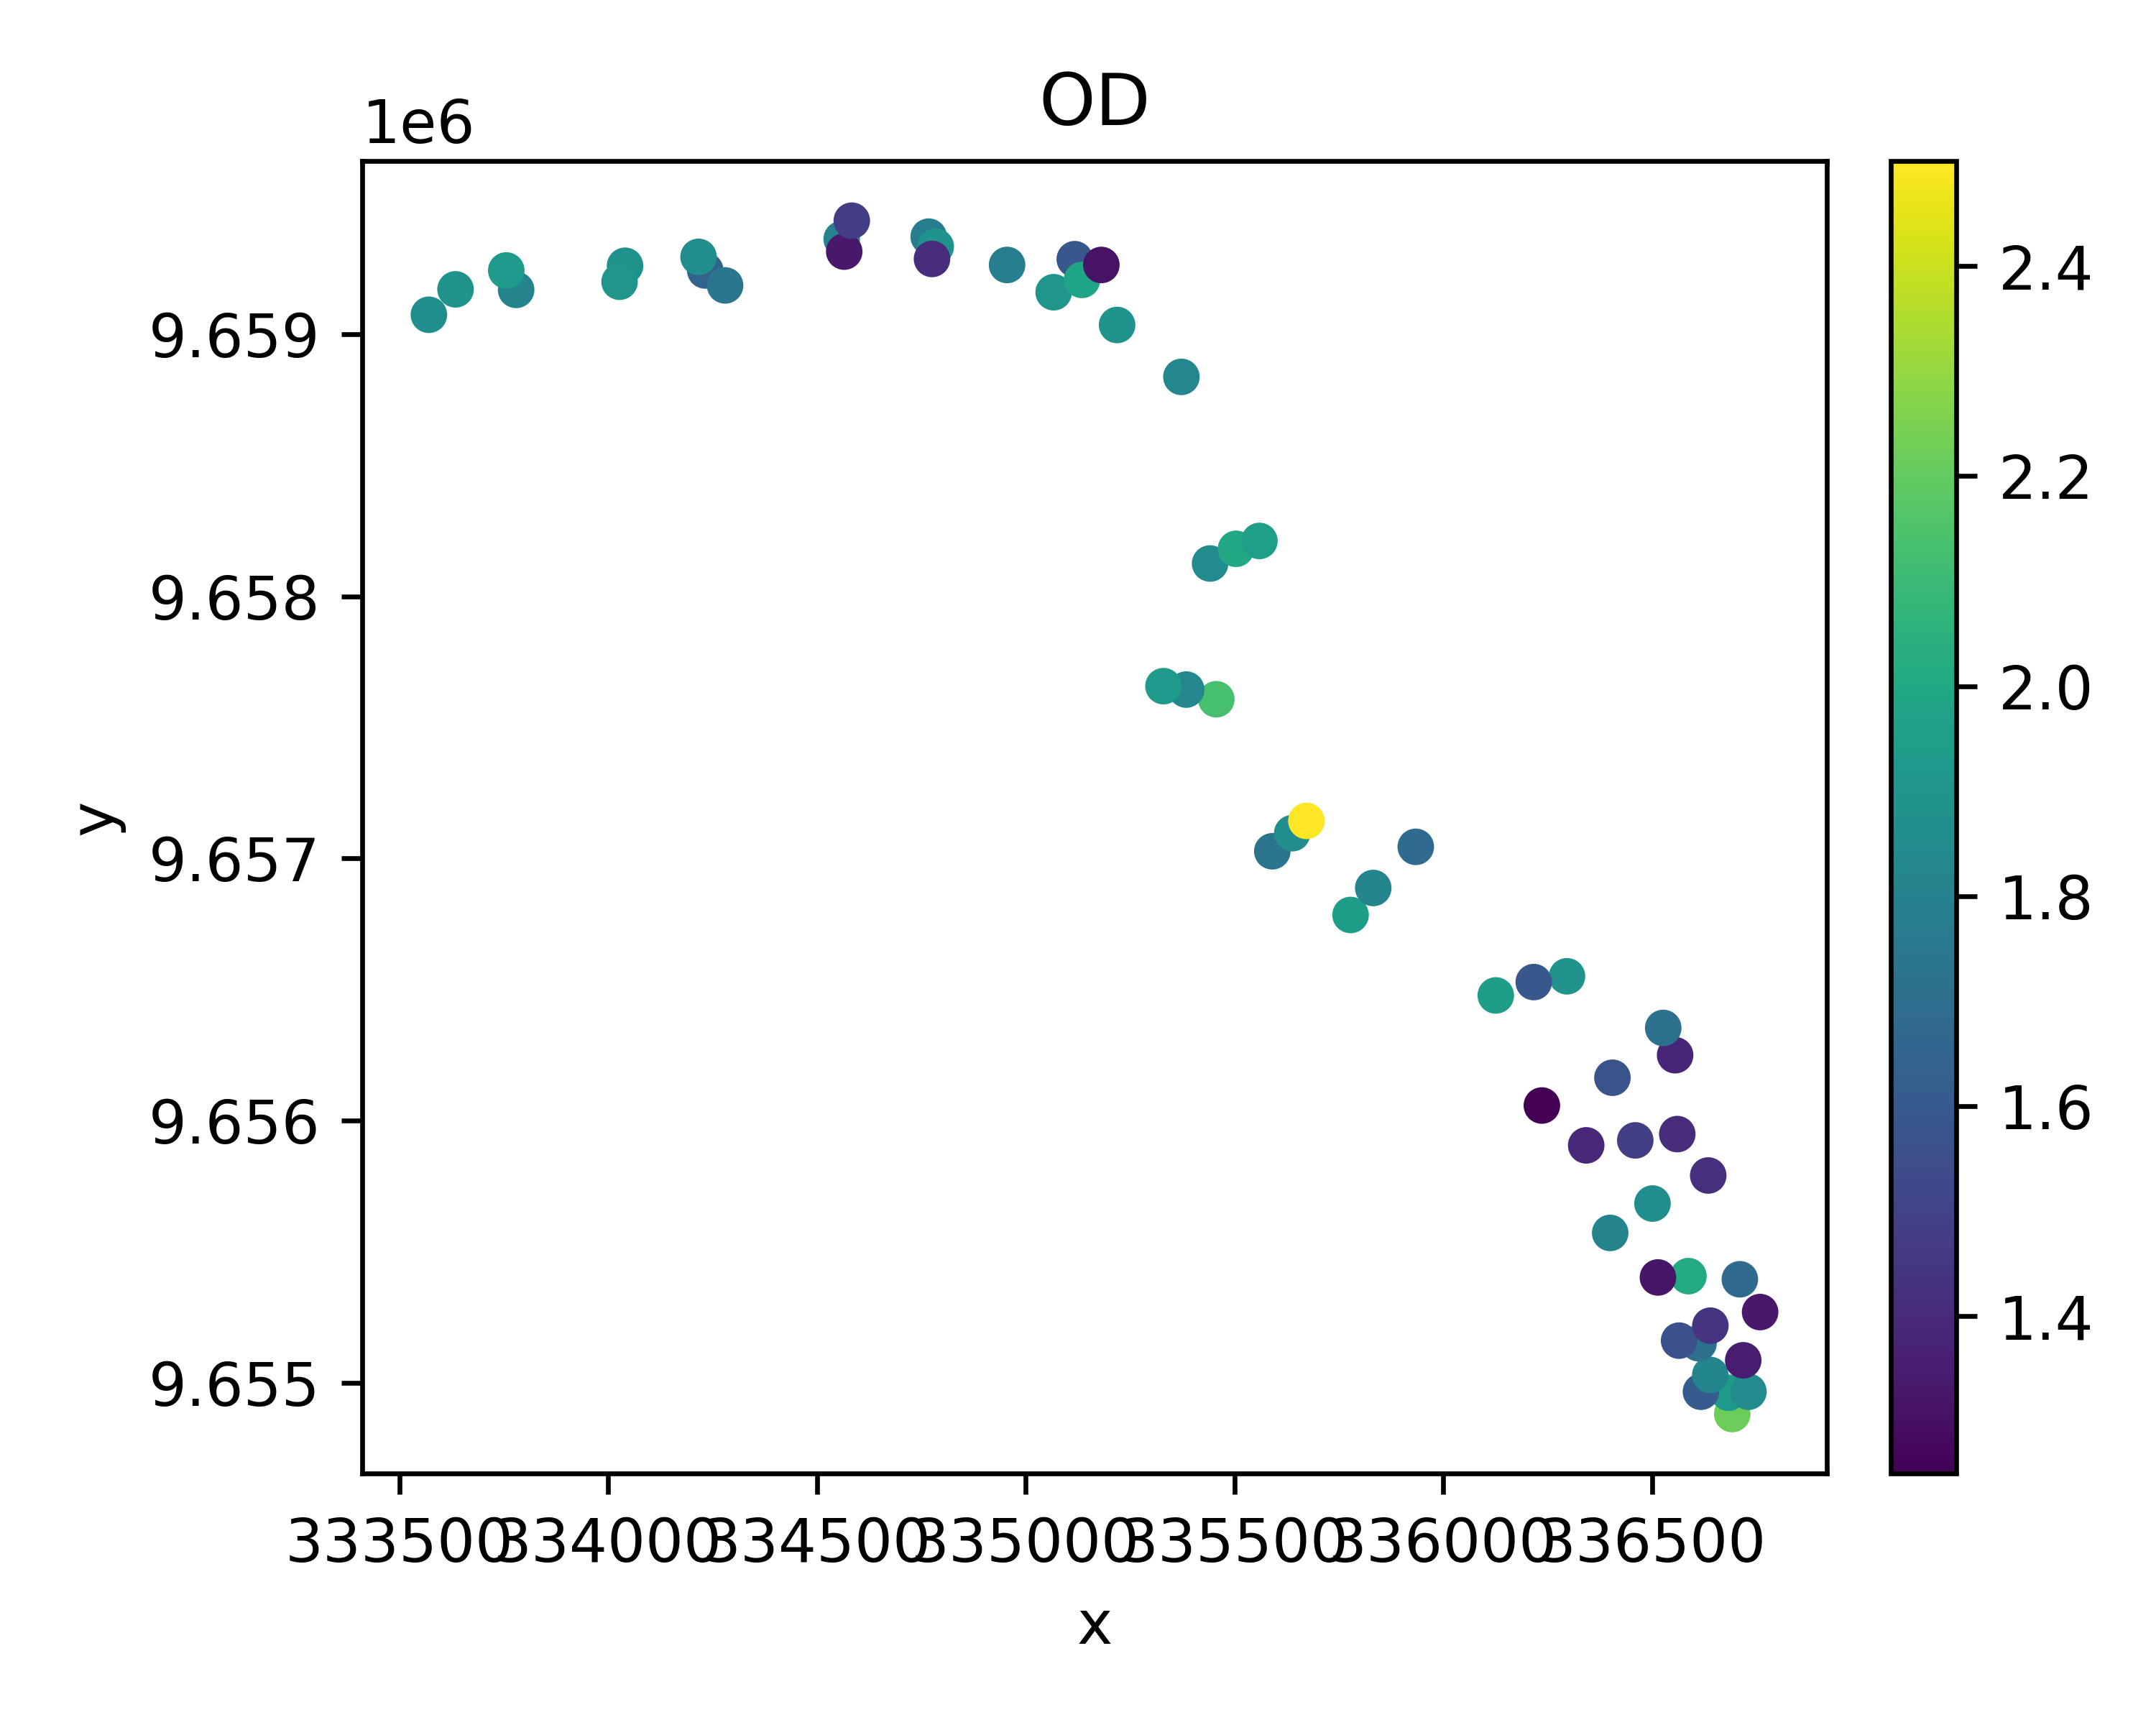
\includegraphics[width=\linewidth]{./figuras/map_OD.png}
		\caption*{(a) Mapa espacial de OD}
	\end{minipage}\hfill
	\begin{minipage}{0.48\textwidth}
		\centering
		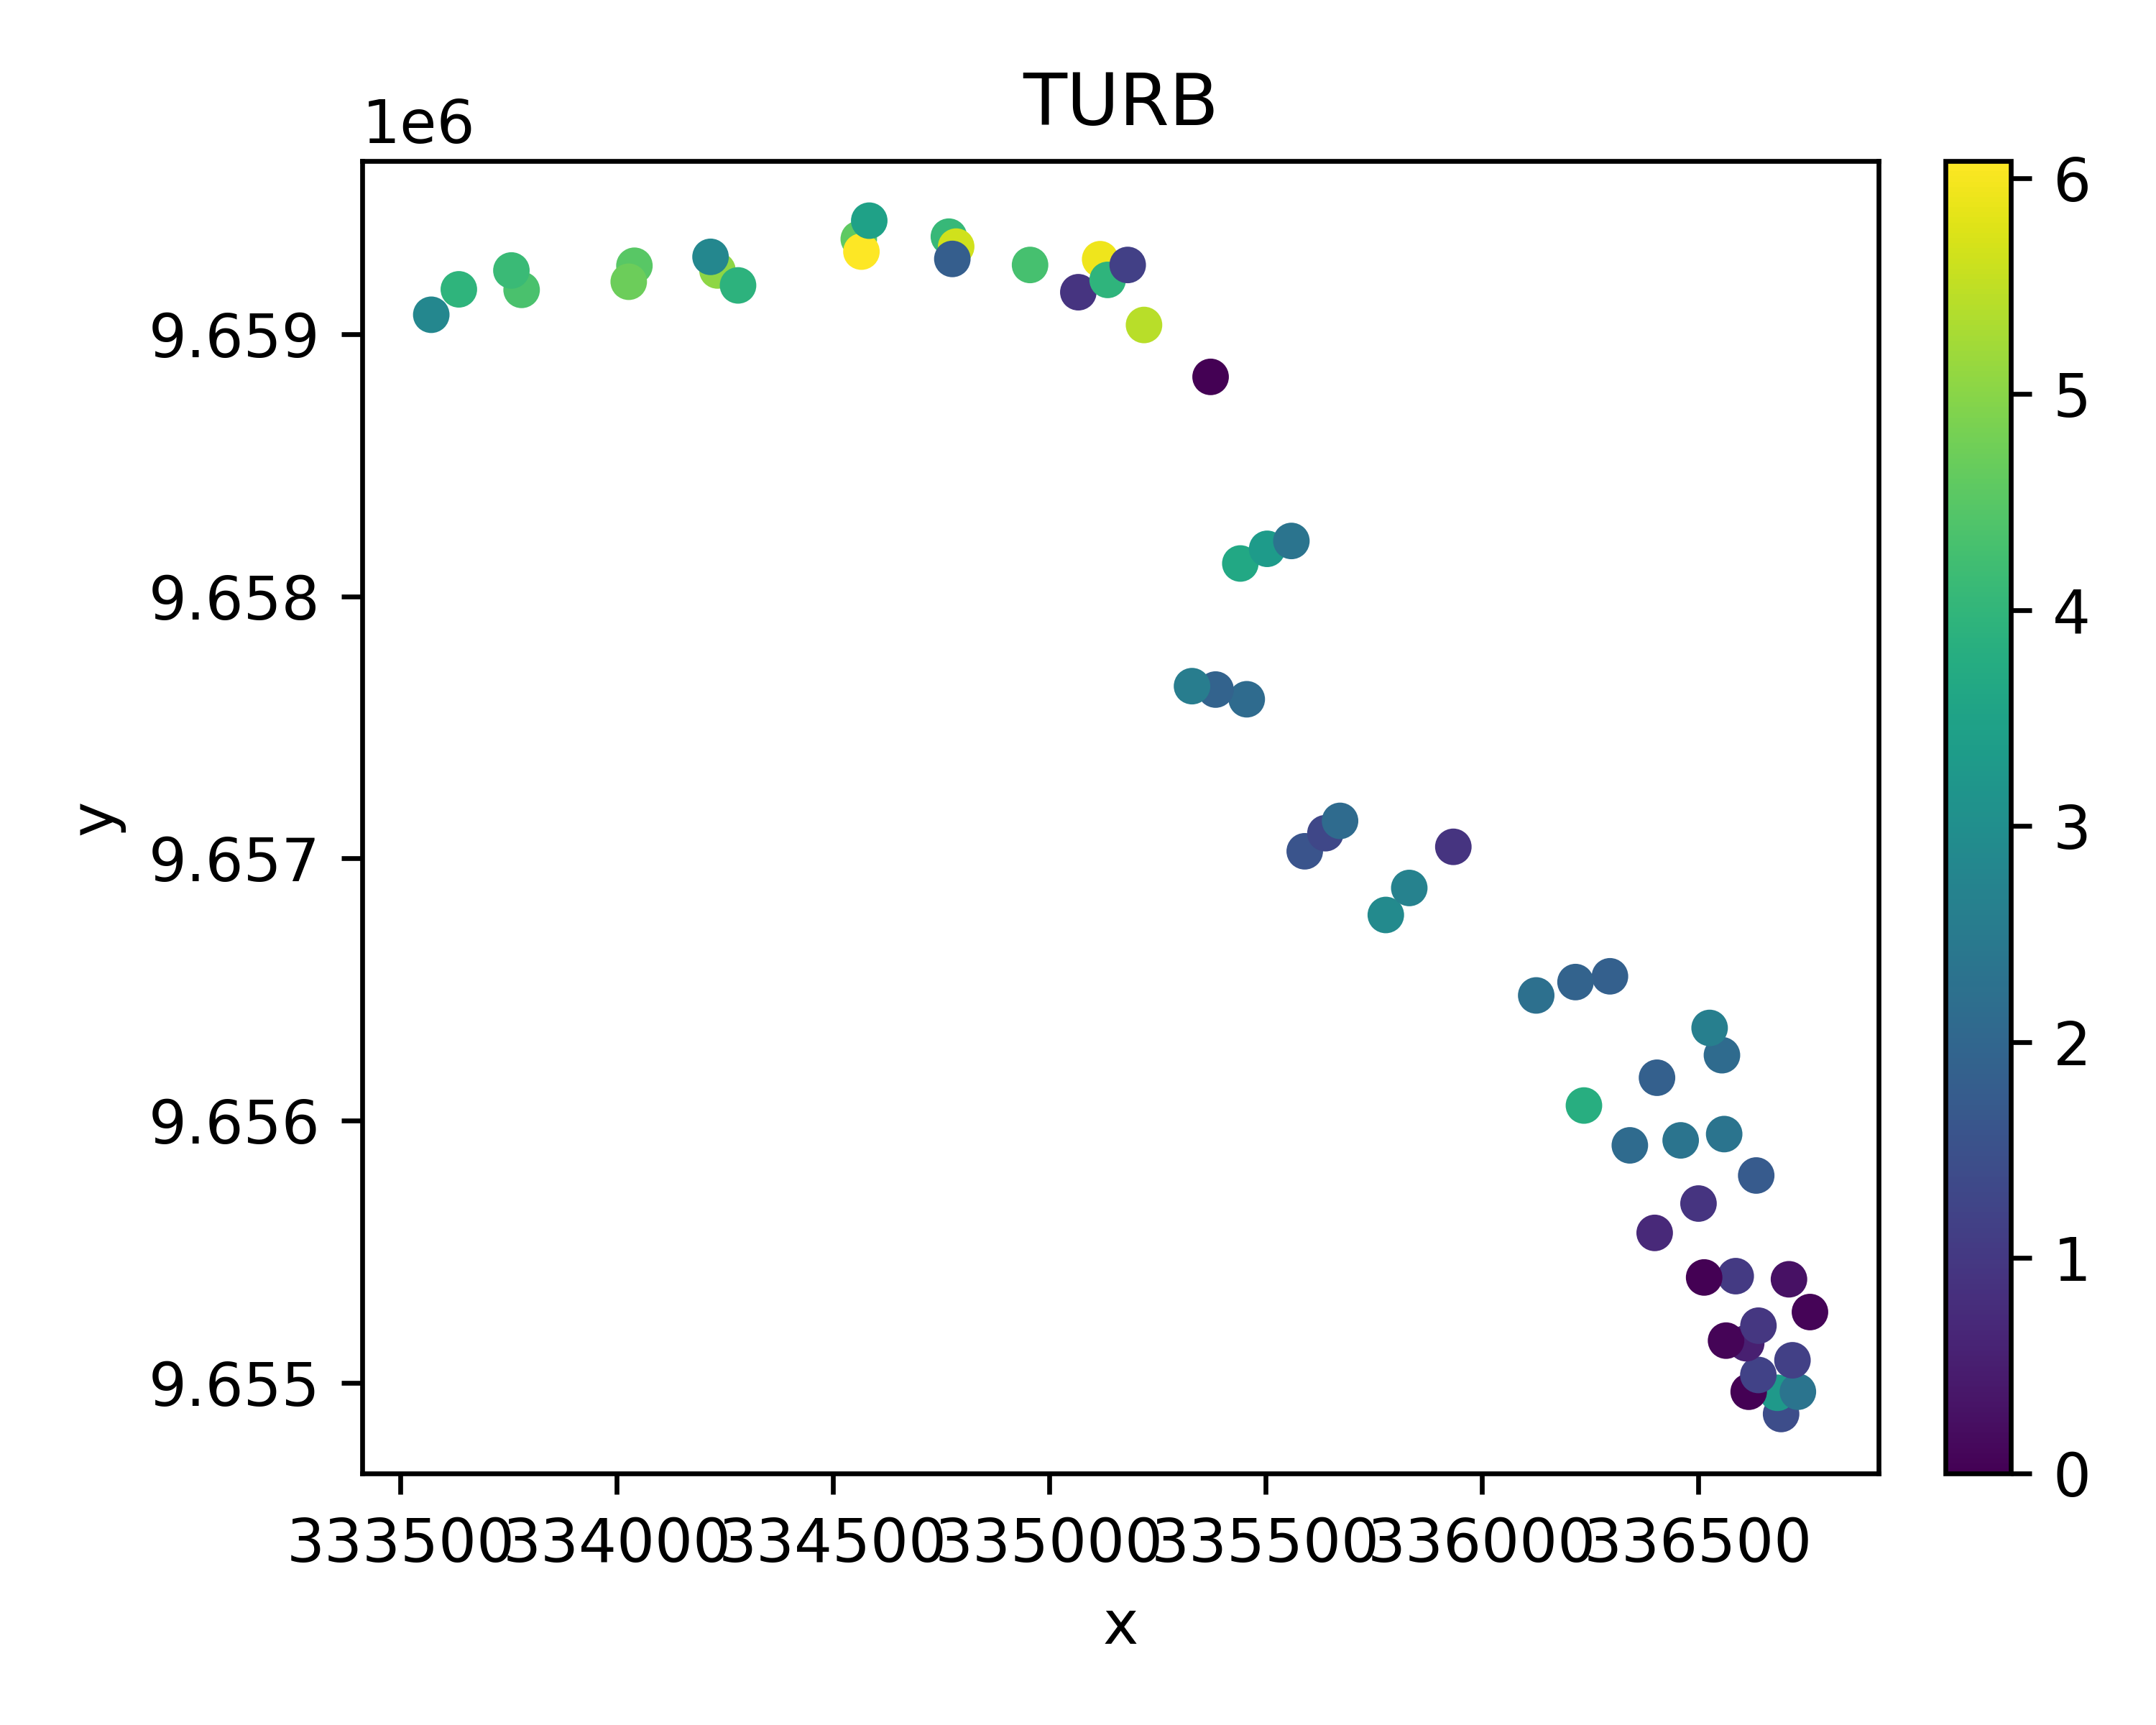
\includegraphics[width=\linewidth]{./figuras/map_TURB.png}
		\caption*{(b) Mapa espacial de turbidez}
	\end{minipage}
	\caption{Padrões espaciais de OD e turbidez.}
	\label{fig:mapas}
\end{figure}

Os mapas de OD e turbidez evidenciam heterogeneidade espacial, com áreas de maior turbidez e zonas
de OD relativamente reduzido. Essa variabilidade sugere influência local de processos físicos e
biogeoquímicos, justificando a necessidade de monitoramento em rede.

\begin{figure}[ht!]
	\centering
	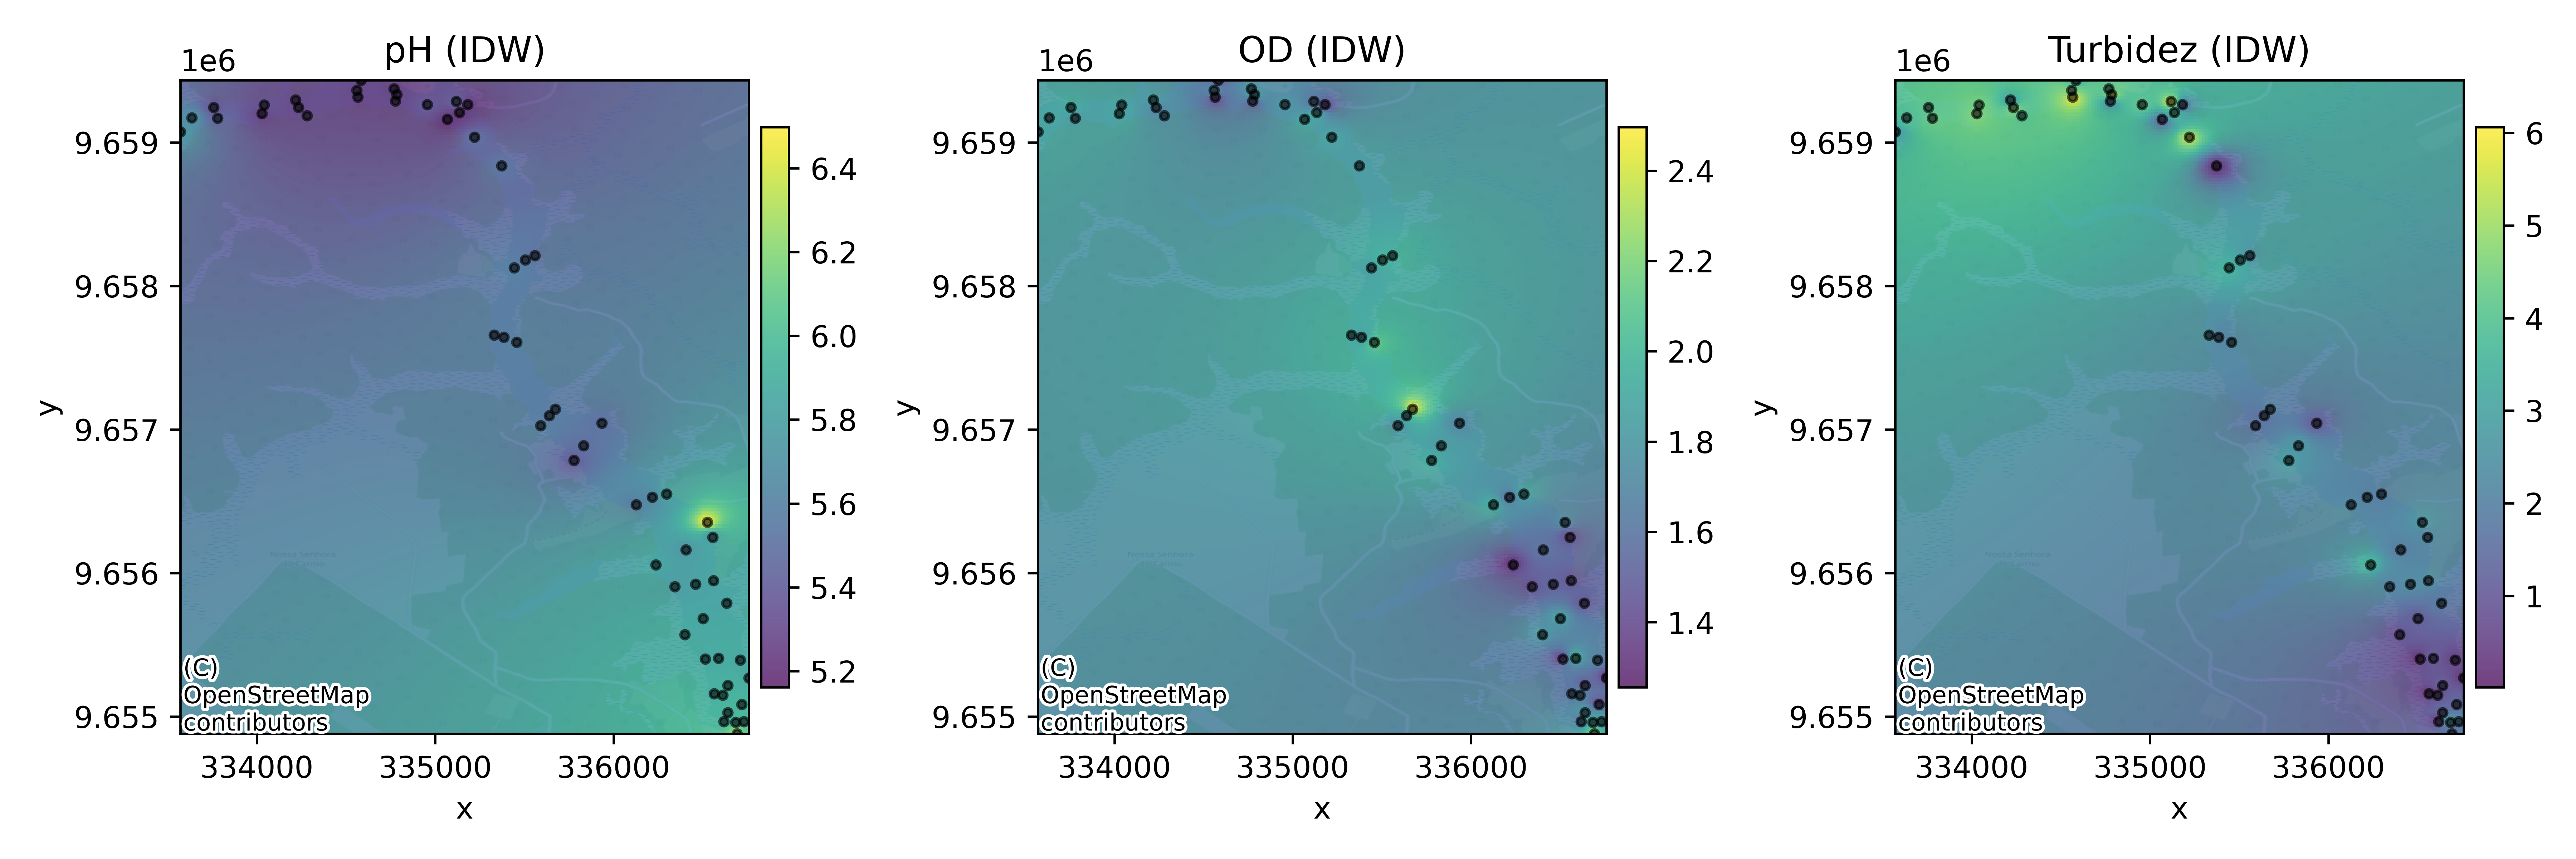
\includegraphics[width=0.98\textwidth]{./figuras/idw_combined.png}
	\caption{Superfícies interpoladas por IDW para pH, OD e turbidez a partir dos
	pontos amostrados.}
	\label{fig:idw}
\end{figure}

A Figura~\ref{fig:idw} apresenta as superfícies interpoladas (IDW) para pH, OD e turbidez, oferecendo
uma leitura contínua das variáveis a partir das medições pontuais. Observam-se gradientes espaciais
consistentes, permitindo identificar regiões com maior contraste entre os parâmetros.

\begin{figure}[ht!]
	\centering
	\begin{minipage}{0.32\textwidth}
		\centering
		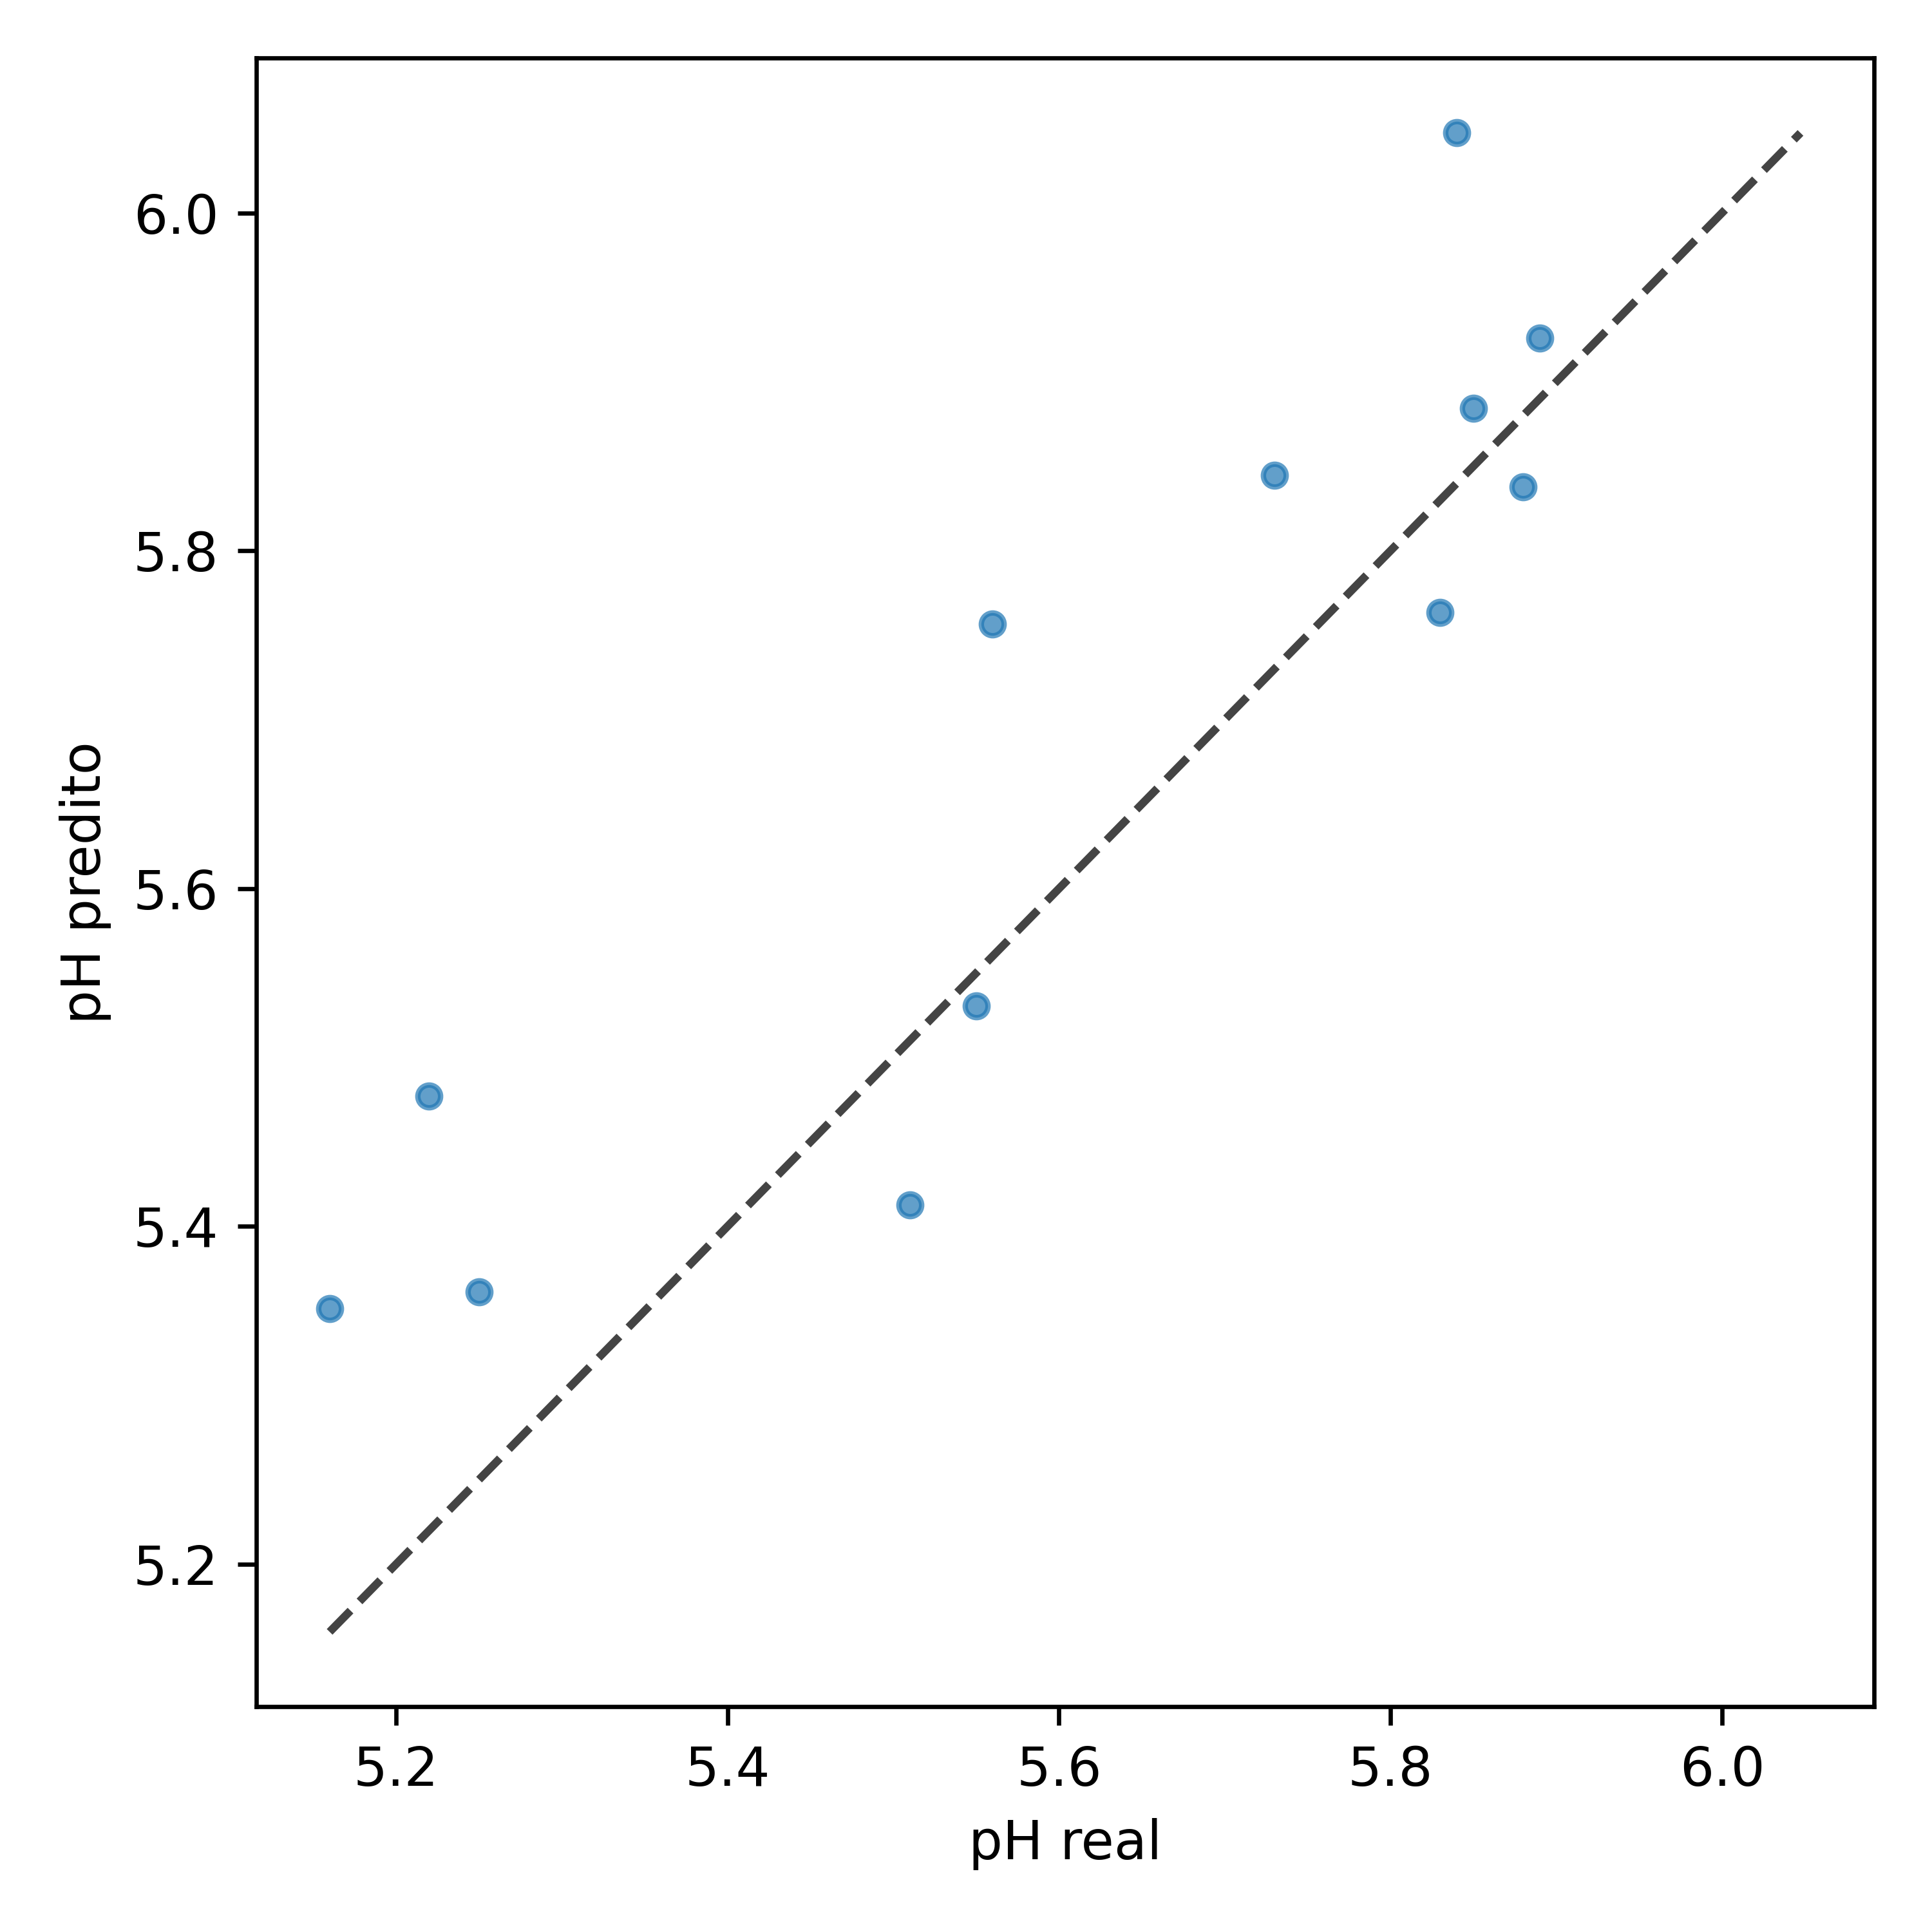
\includegraphics[width=\linewidth]{./figuras/pred_vs_real_pH_multi.png}
		\caption*{(a) pH}
	\end{minipage}\hfill
	\begin{minipage}{0.32\textwidth}
		\centering
		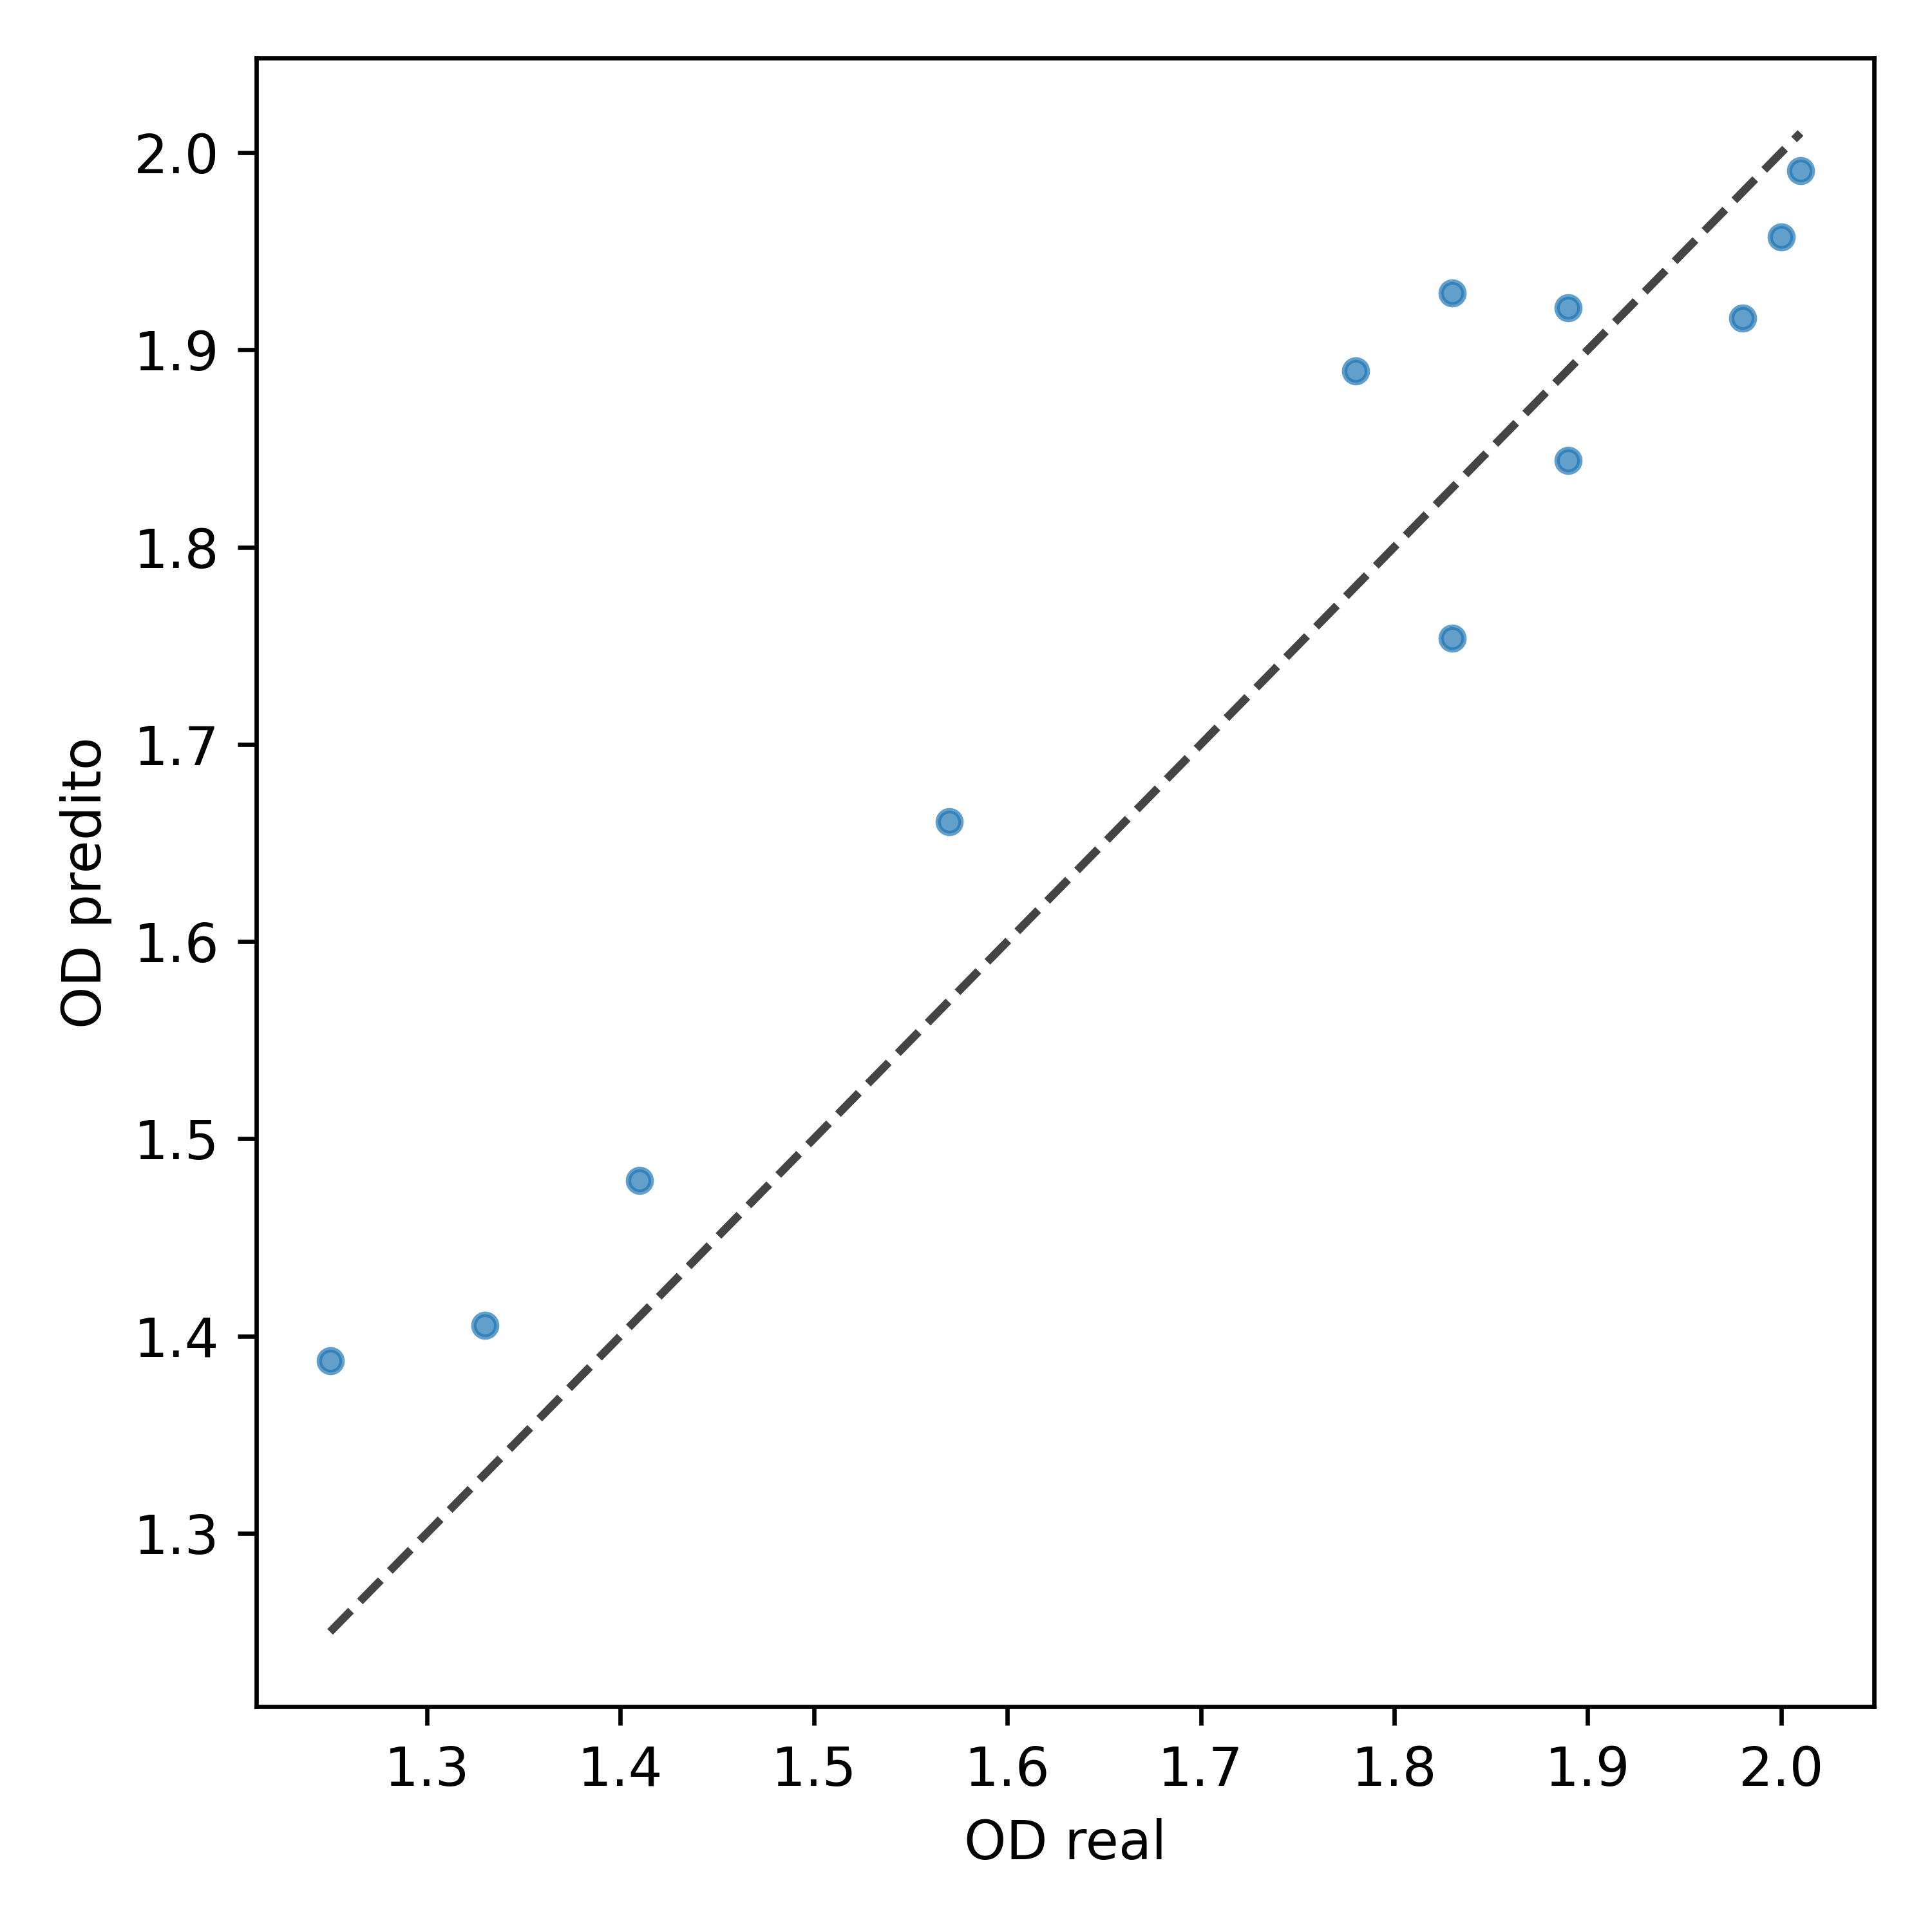
\includegraphics[width=\linewidth]{./figuras/pred_vs_real_OD_multi.png}
		\caption*{(b) OD}
	\end{minipage}\hfill
	\begin{minipage}{0.32\textwidth}
		\centering
		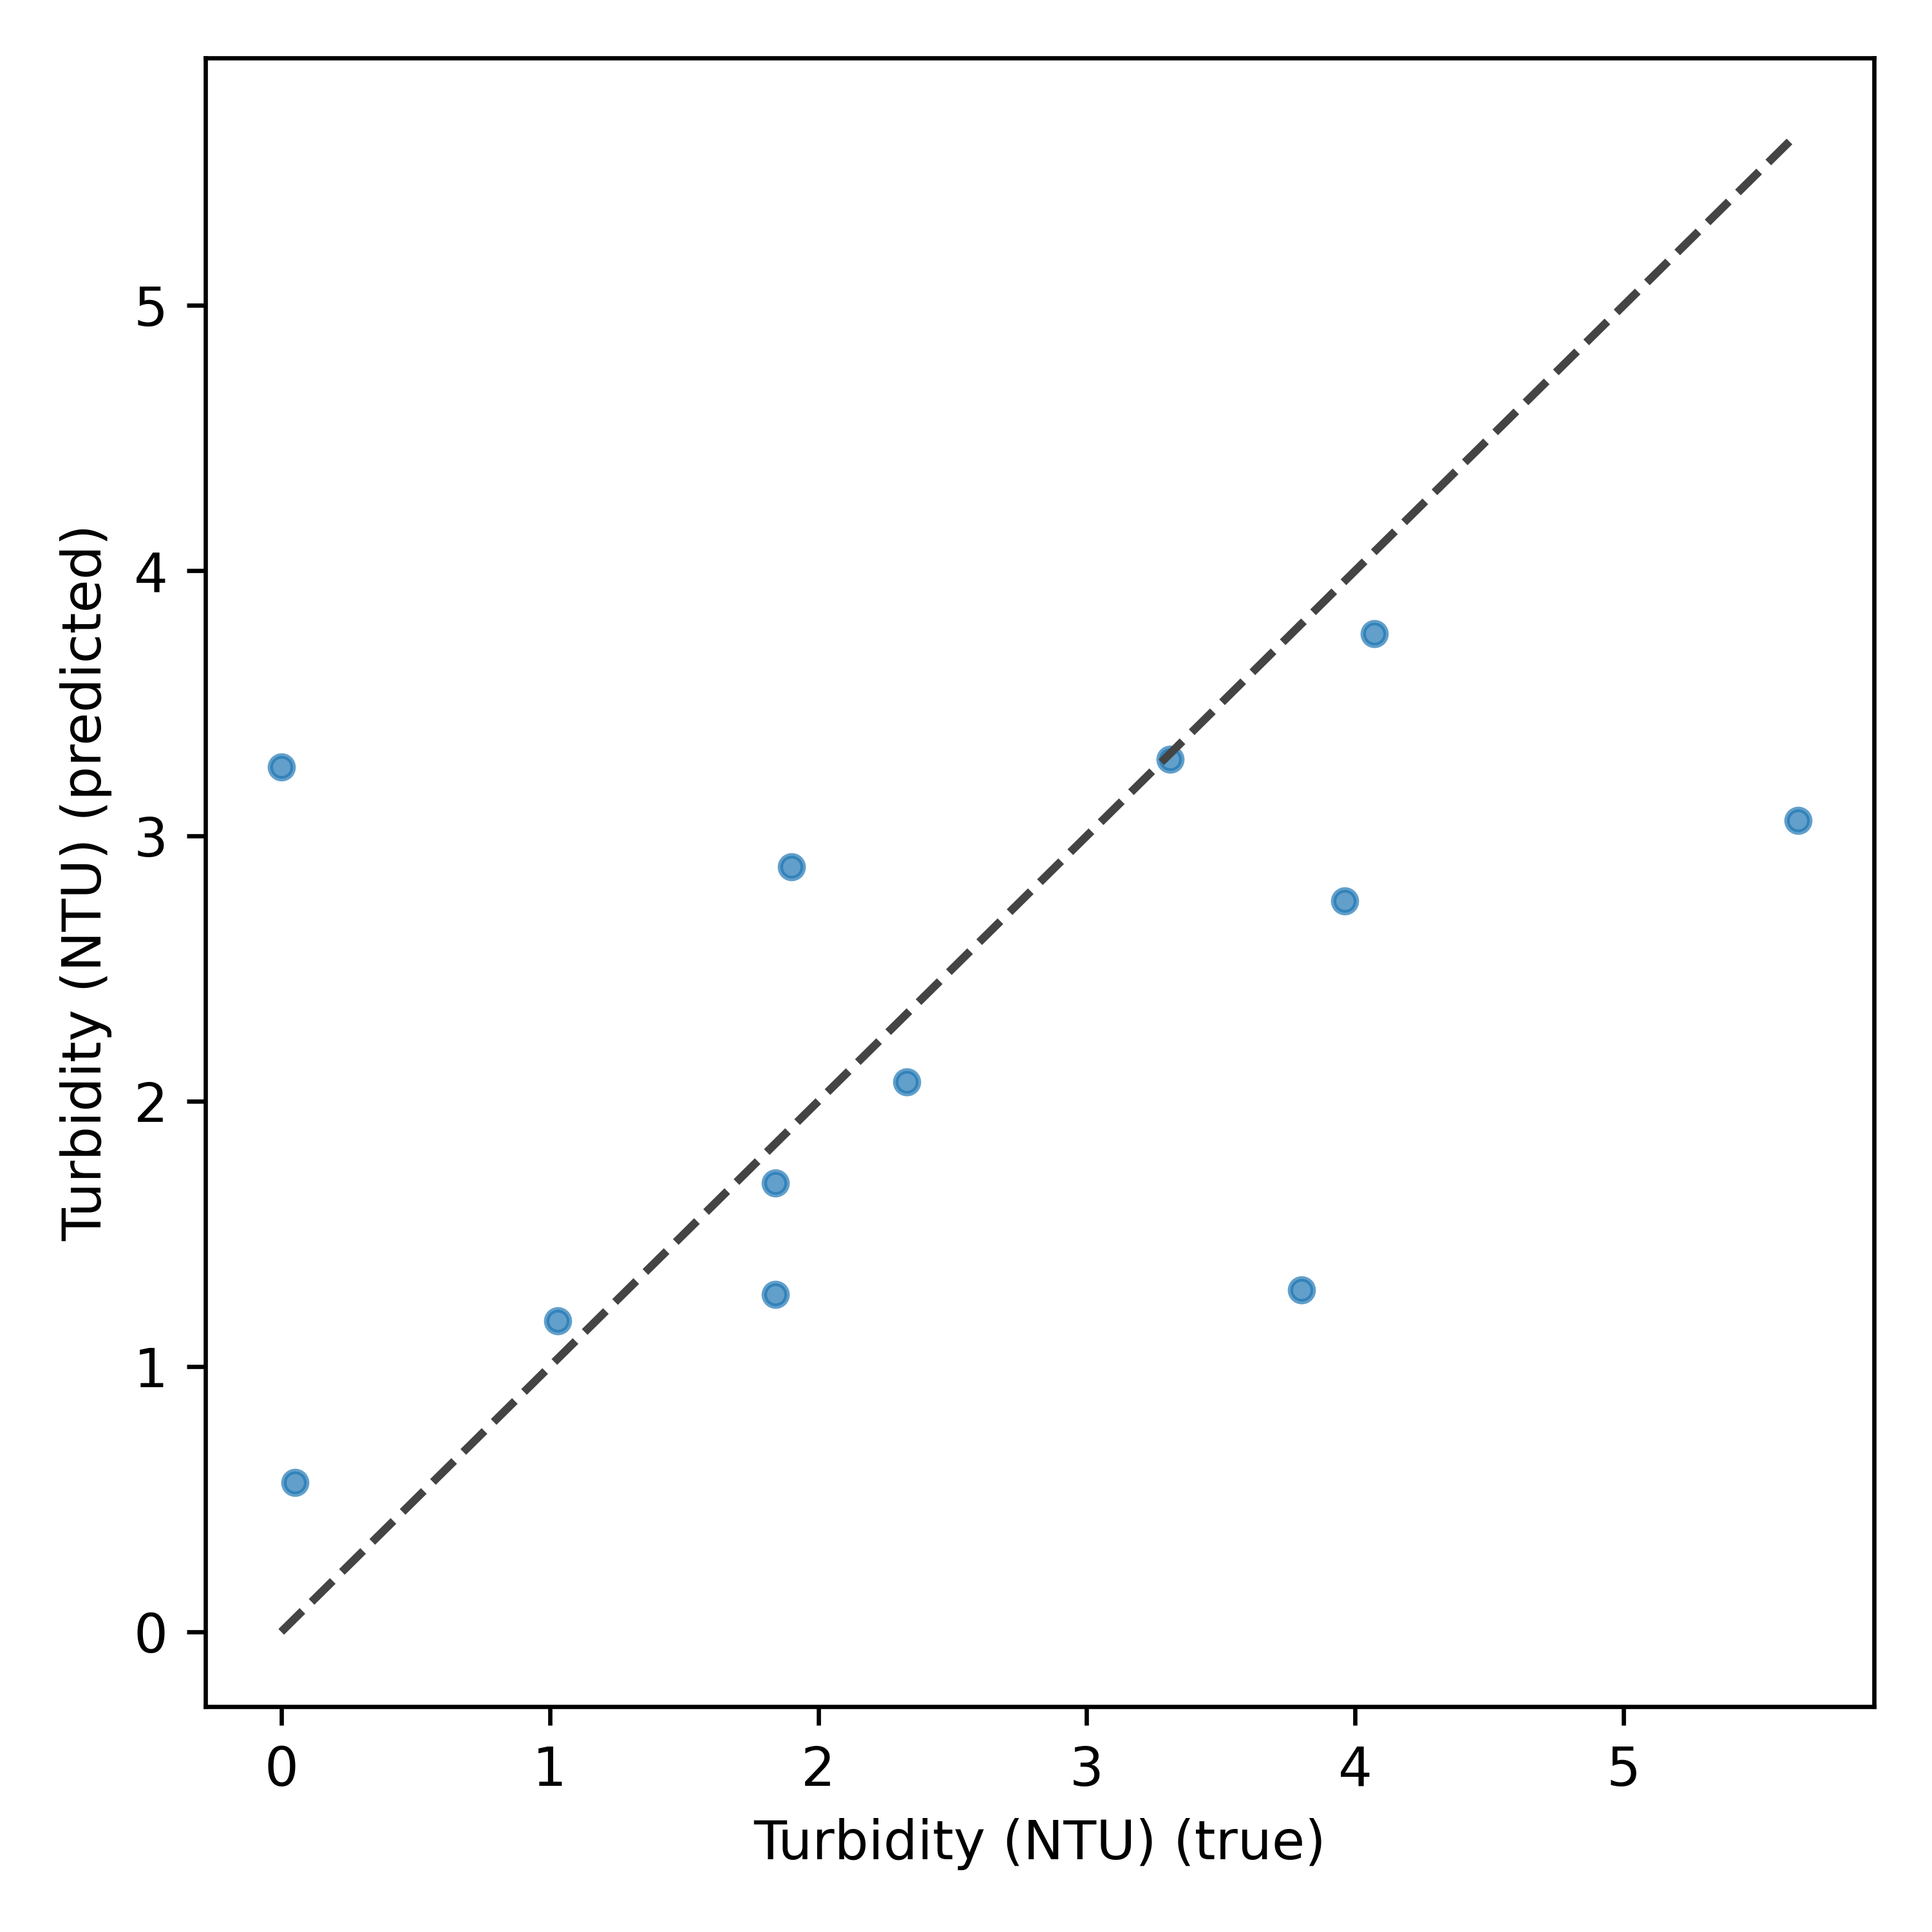
\includegraphics[width=\linewidth]{./figuras/pred_vs_real_TURB_multi.png}
		\caption*{(c) Turbidez}
	\end{minipage}
	\caption{Predito vs. real do modelo multimodal para pH, OD e turbidez.}
	\label{fig:multi_pred}
\end{figure}

Na Figura~\ref{fig:multi_pred}, o ajuste multimodal apresenta boa aderência para pH e OD, enquanto a
turbidez apresenta maior dispersão. Ainda assim, a tendência geral permanece alinhada à linha de
identidade, indicando capacidade preditiva satisfatória em múltiplas variáveis.

\begin{figure}[ht!]
	\centering
	\begin{minipage}{0.32\textwidth}
		\centering
		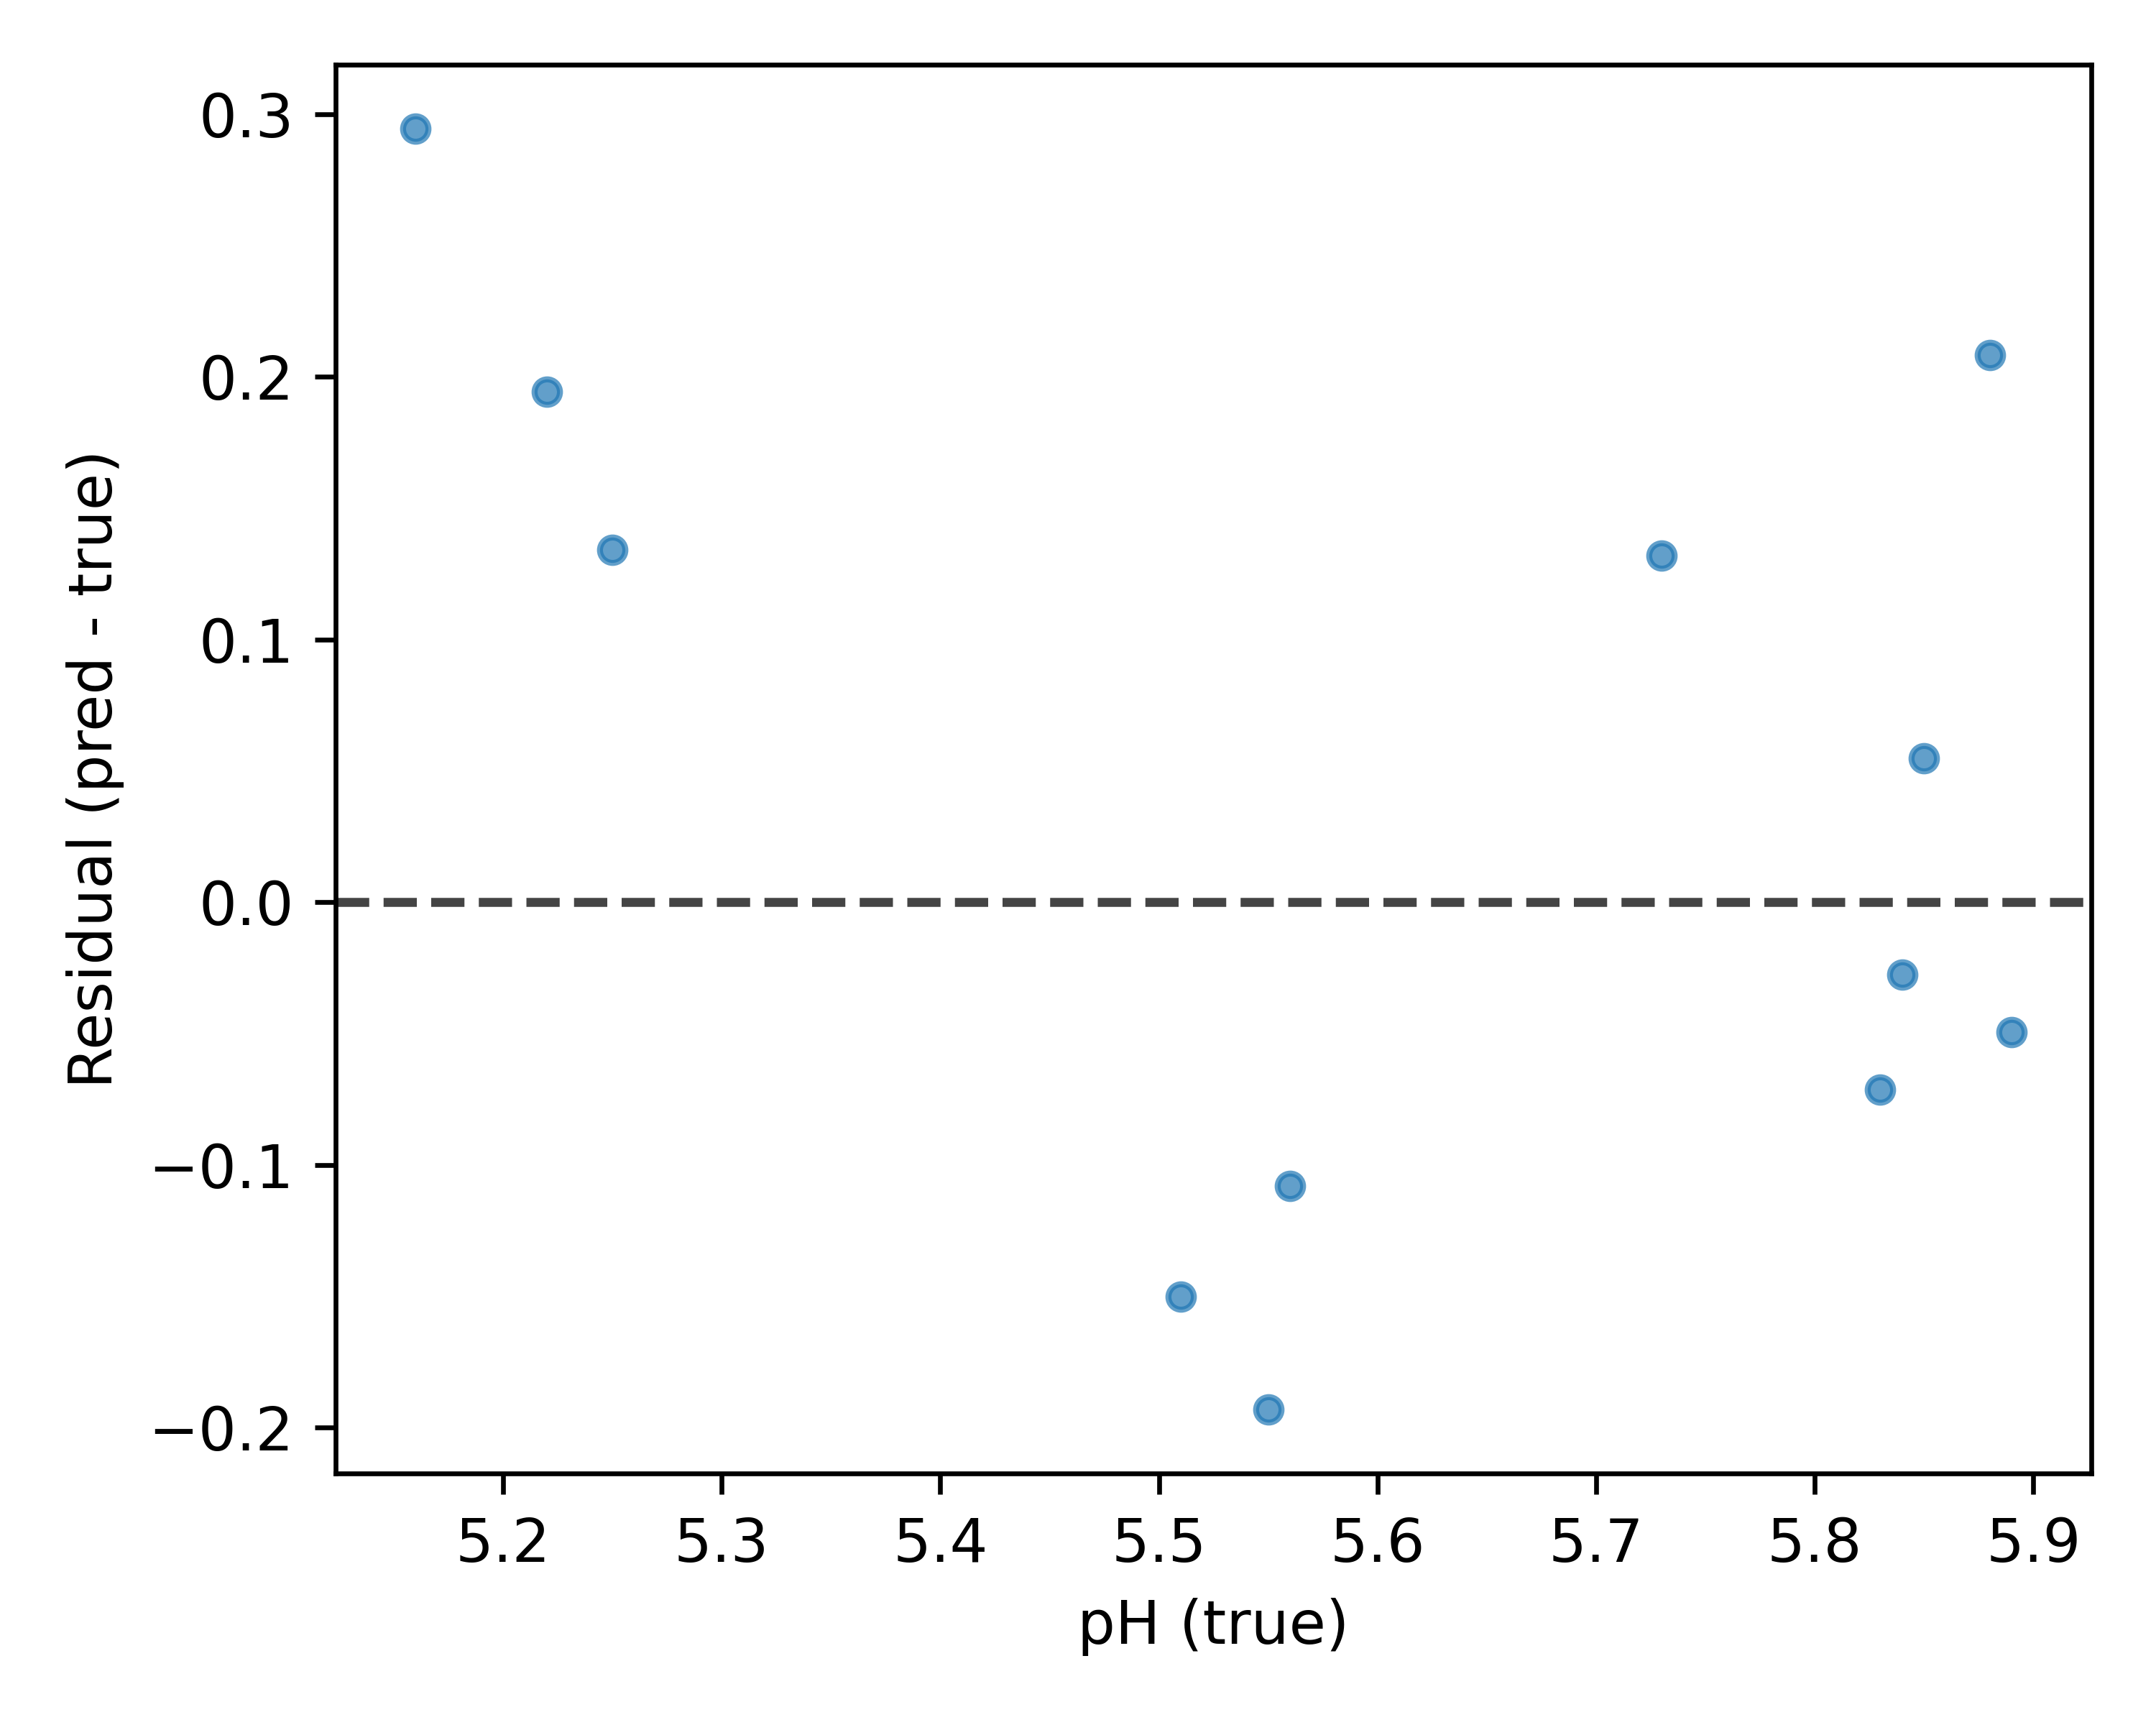
\includegraphics[width=\linewidth]{./figuras/residuals_pH_multi.png}
		\caption*{(a) pH}
	\end{minipage}\hfill
	\begin{minipage}{0.32\textwidth}
		\centering
		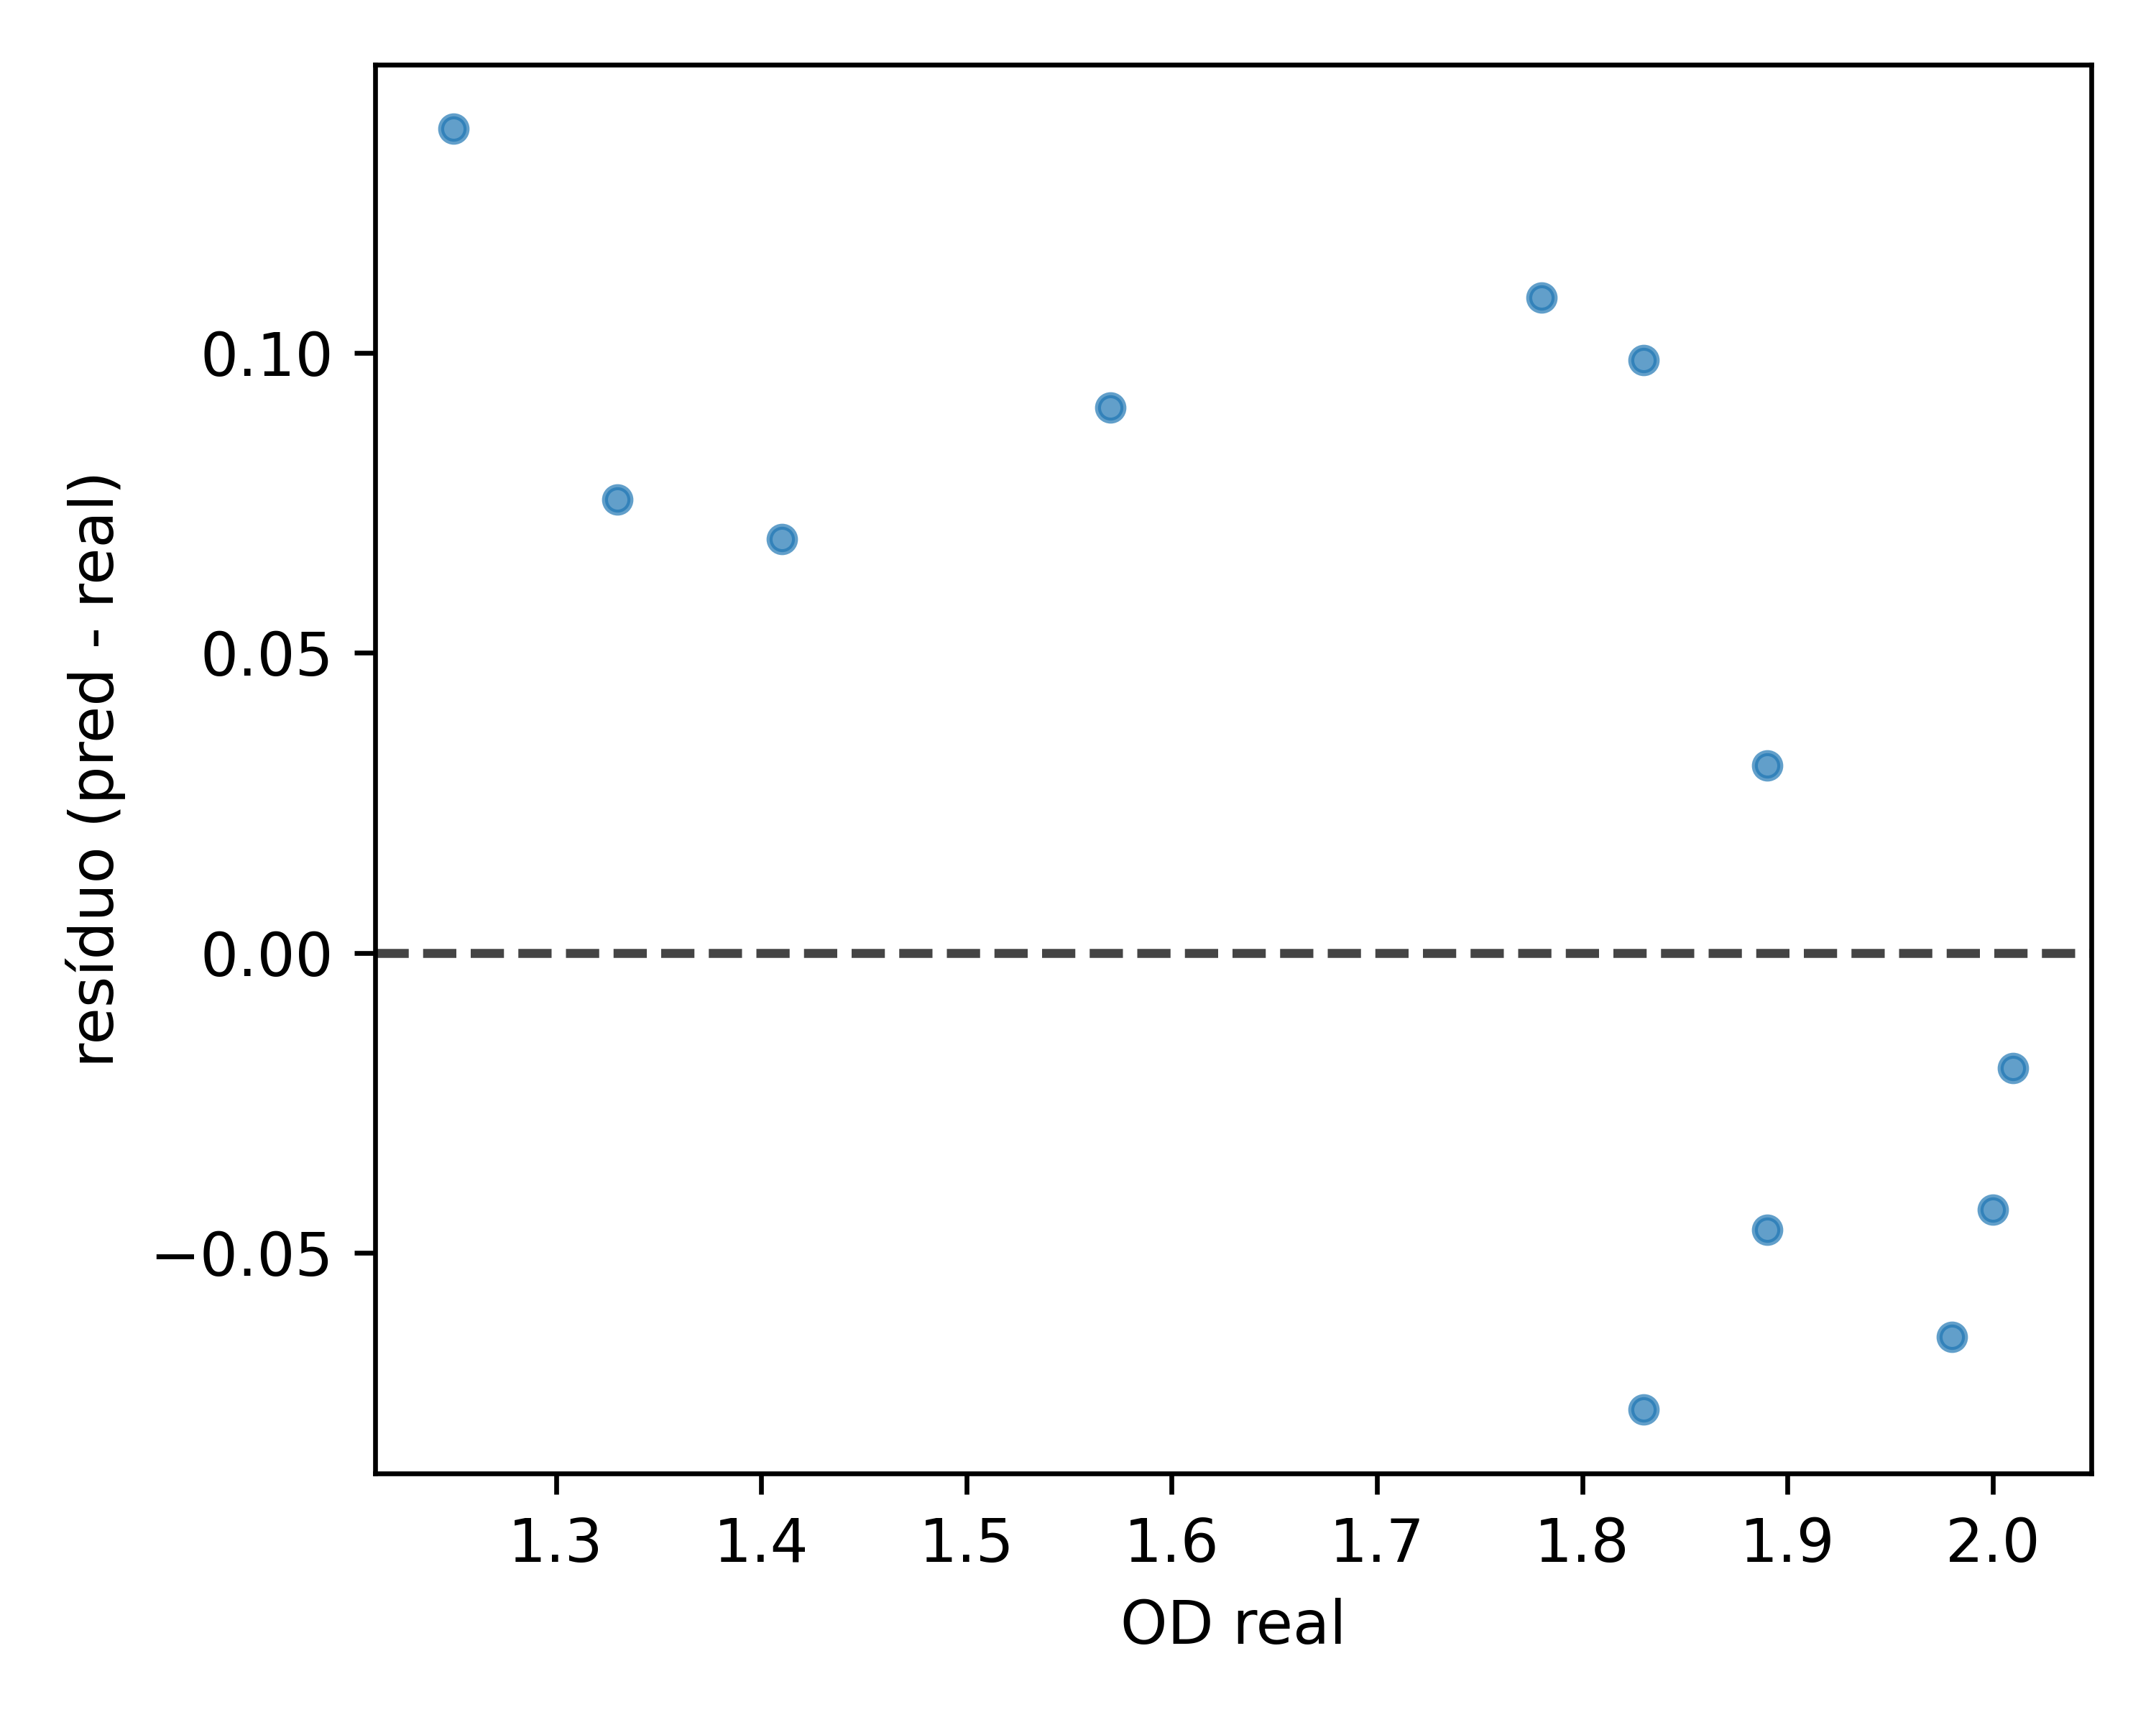
\includegraphics[width=\linewidth]{./figuras/residuals_OD_multi.png}
		\caption*{(b) OD}
	\end{minipage}\hfill
	\begin{minipage}{0.32\textwidth}
		\centering
		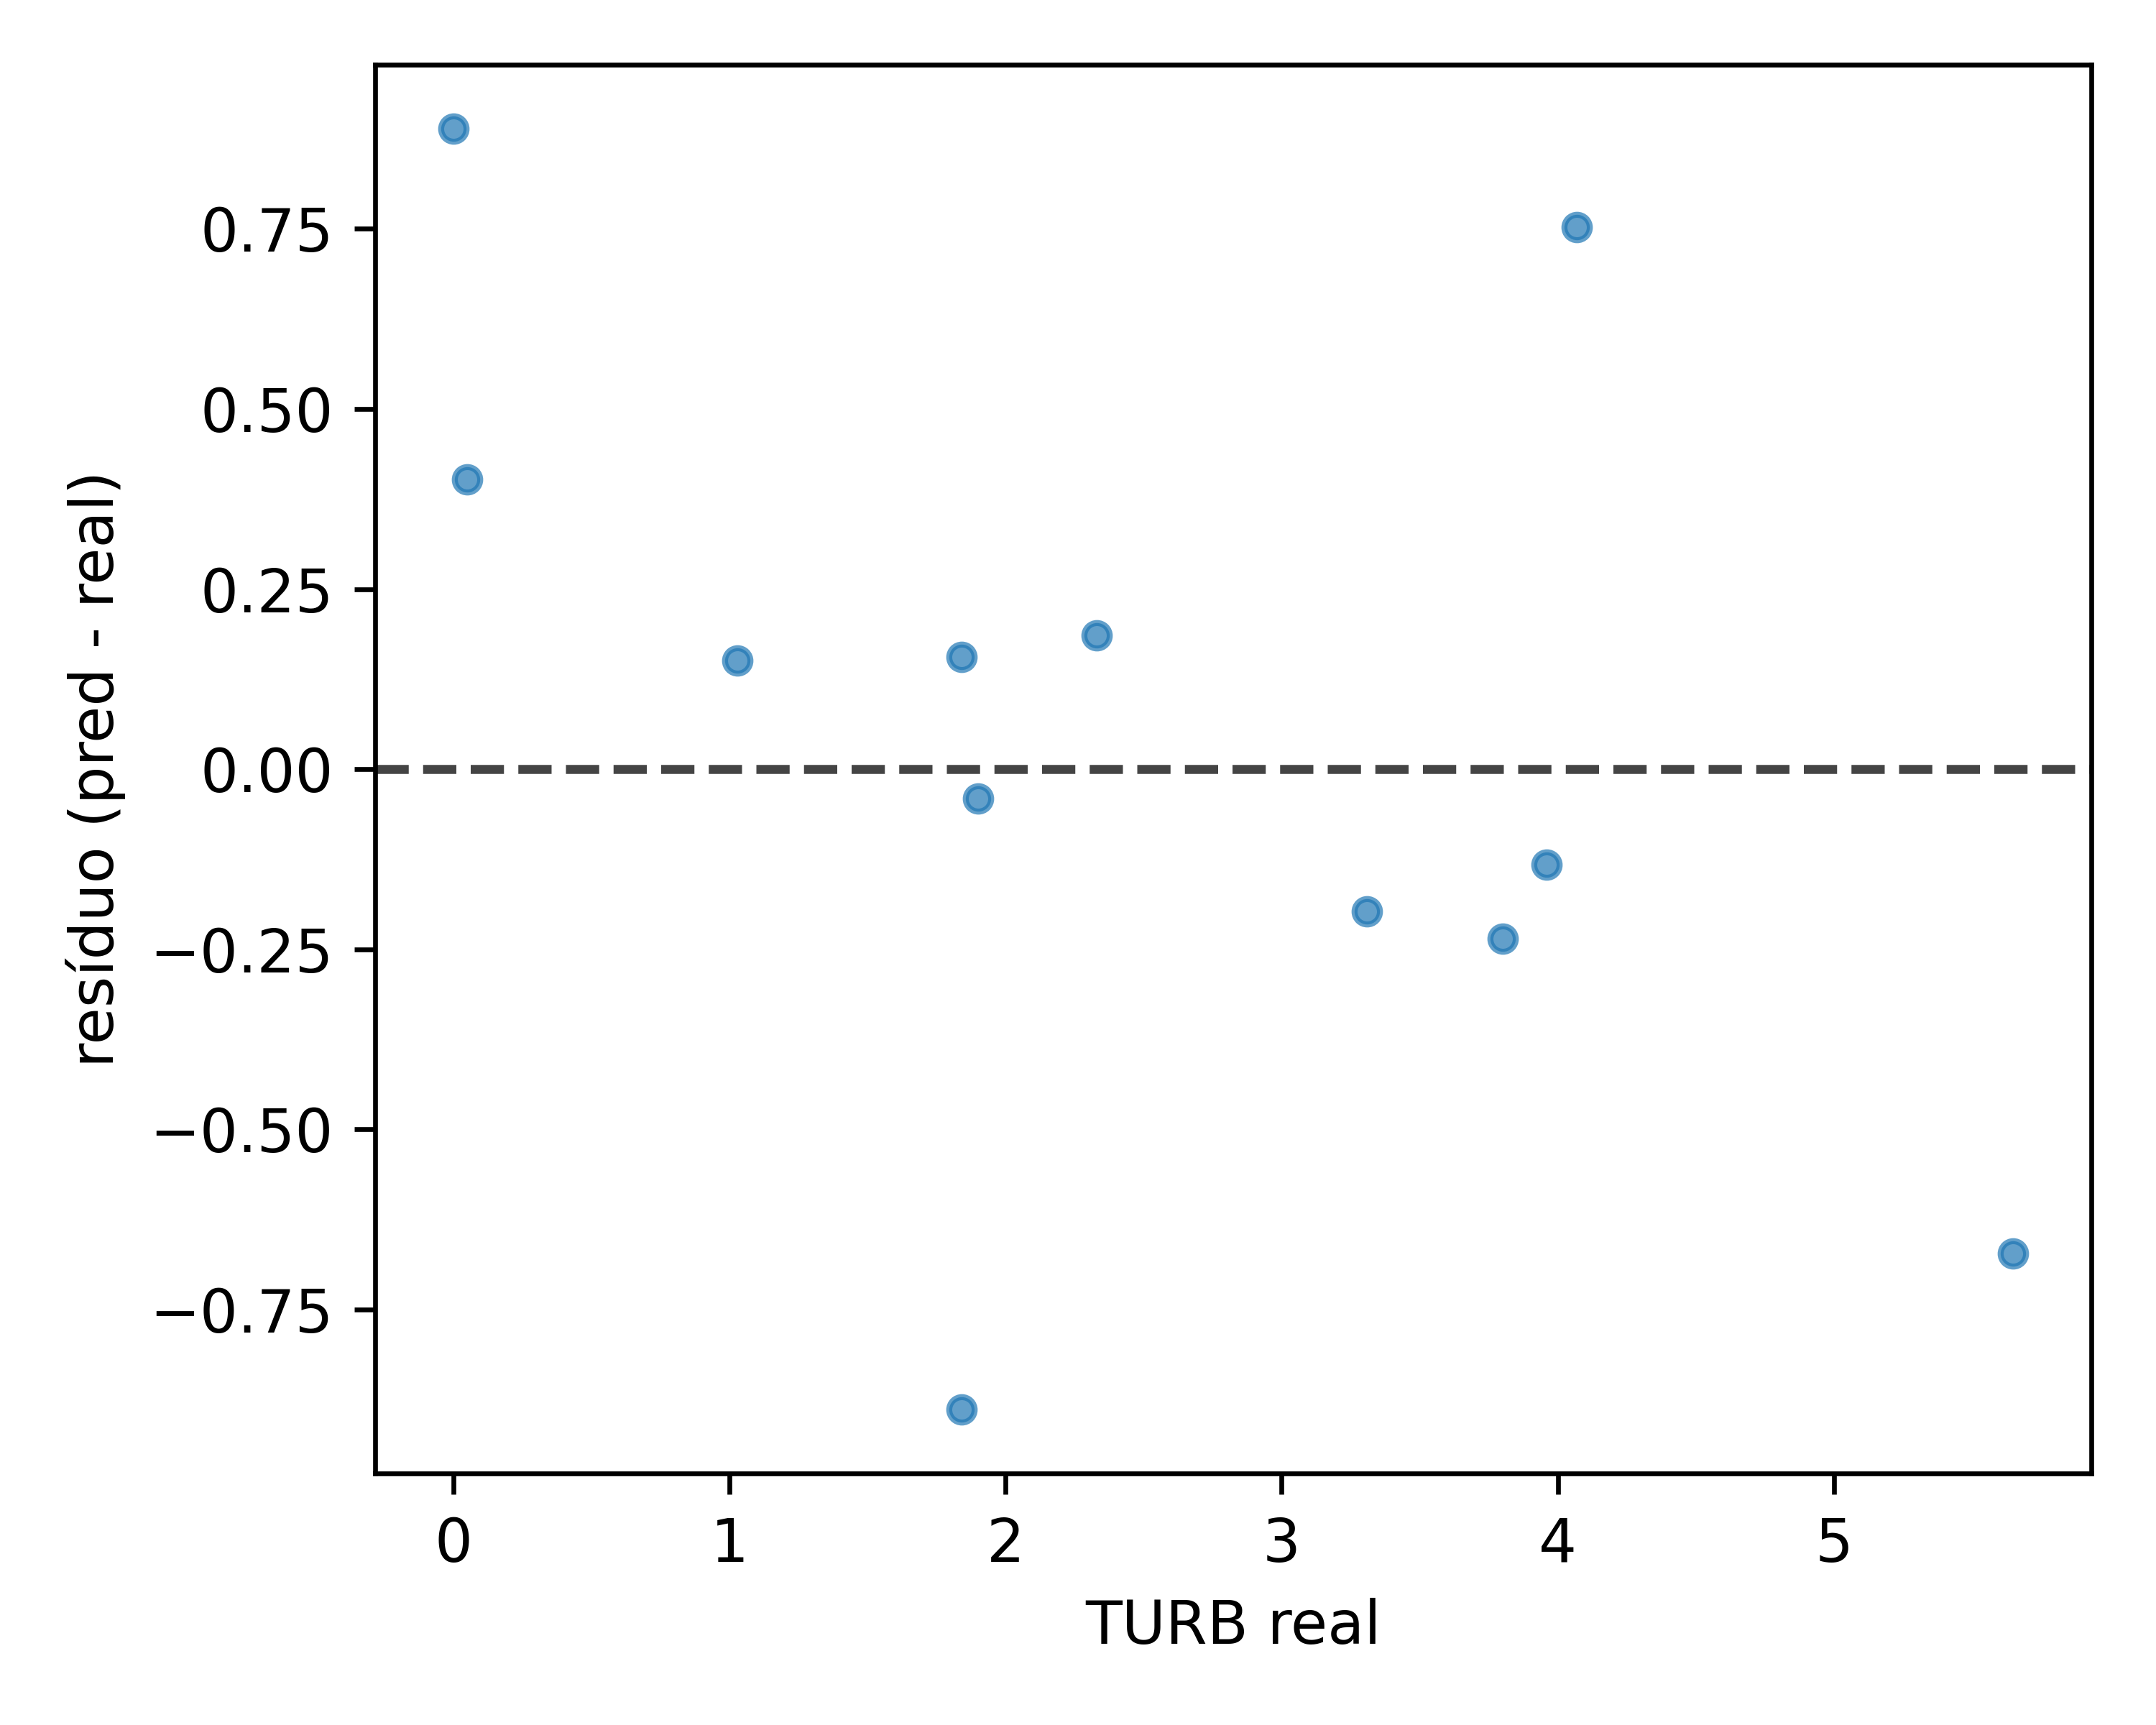
\includegraphics[width=\linewidth]{./figuras/residuals_TURB_multi.png}
		\caption*{(c) Turbidez}
	\end{minipage}
	\caption{Resíduos (predito - real) do modelo multimodal para cada variável.}
	\label{fig:multi_res}
\end{figure}

Os resíduos na Figura~\ref{fig:multi_res} se distribuem em torno de zero para pH e OD, sugerindo
ausência de viés sistemático relevante. Para turbidez, há maior variabilidade, indicando maior
dificuldade de modelagem e possível necessidade de mais dados ou calibração adicional.

\begin{figure}[ht!]
	\centering
	\begin{minipage}{0.48\textwidth}
		\centering
		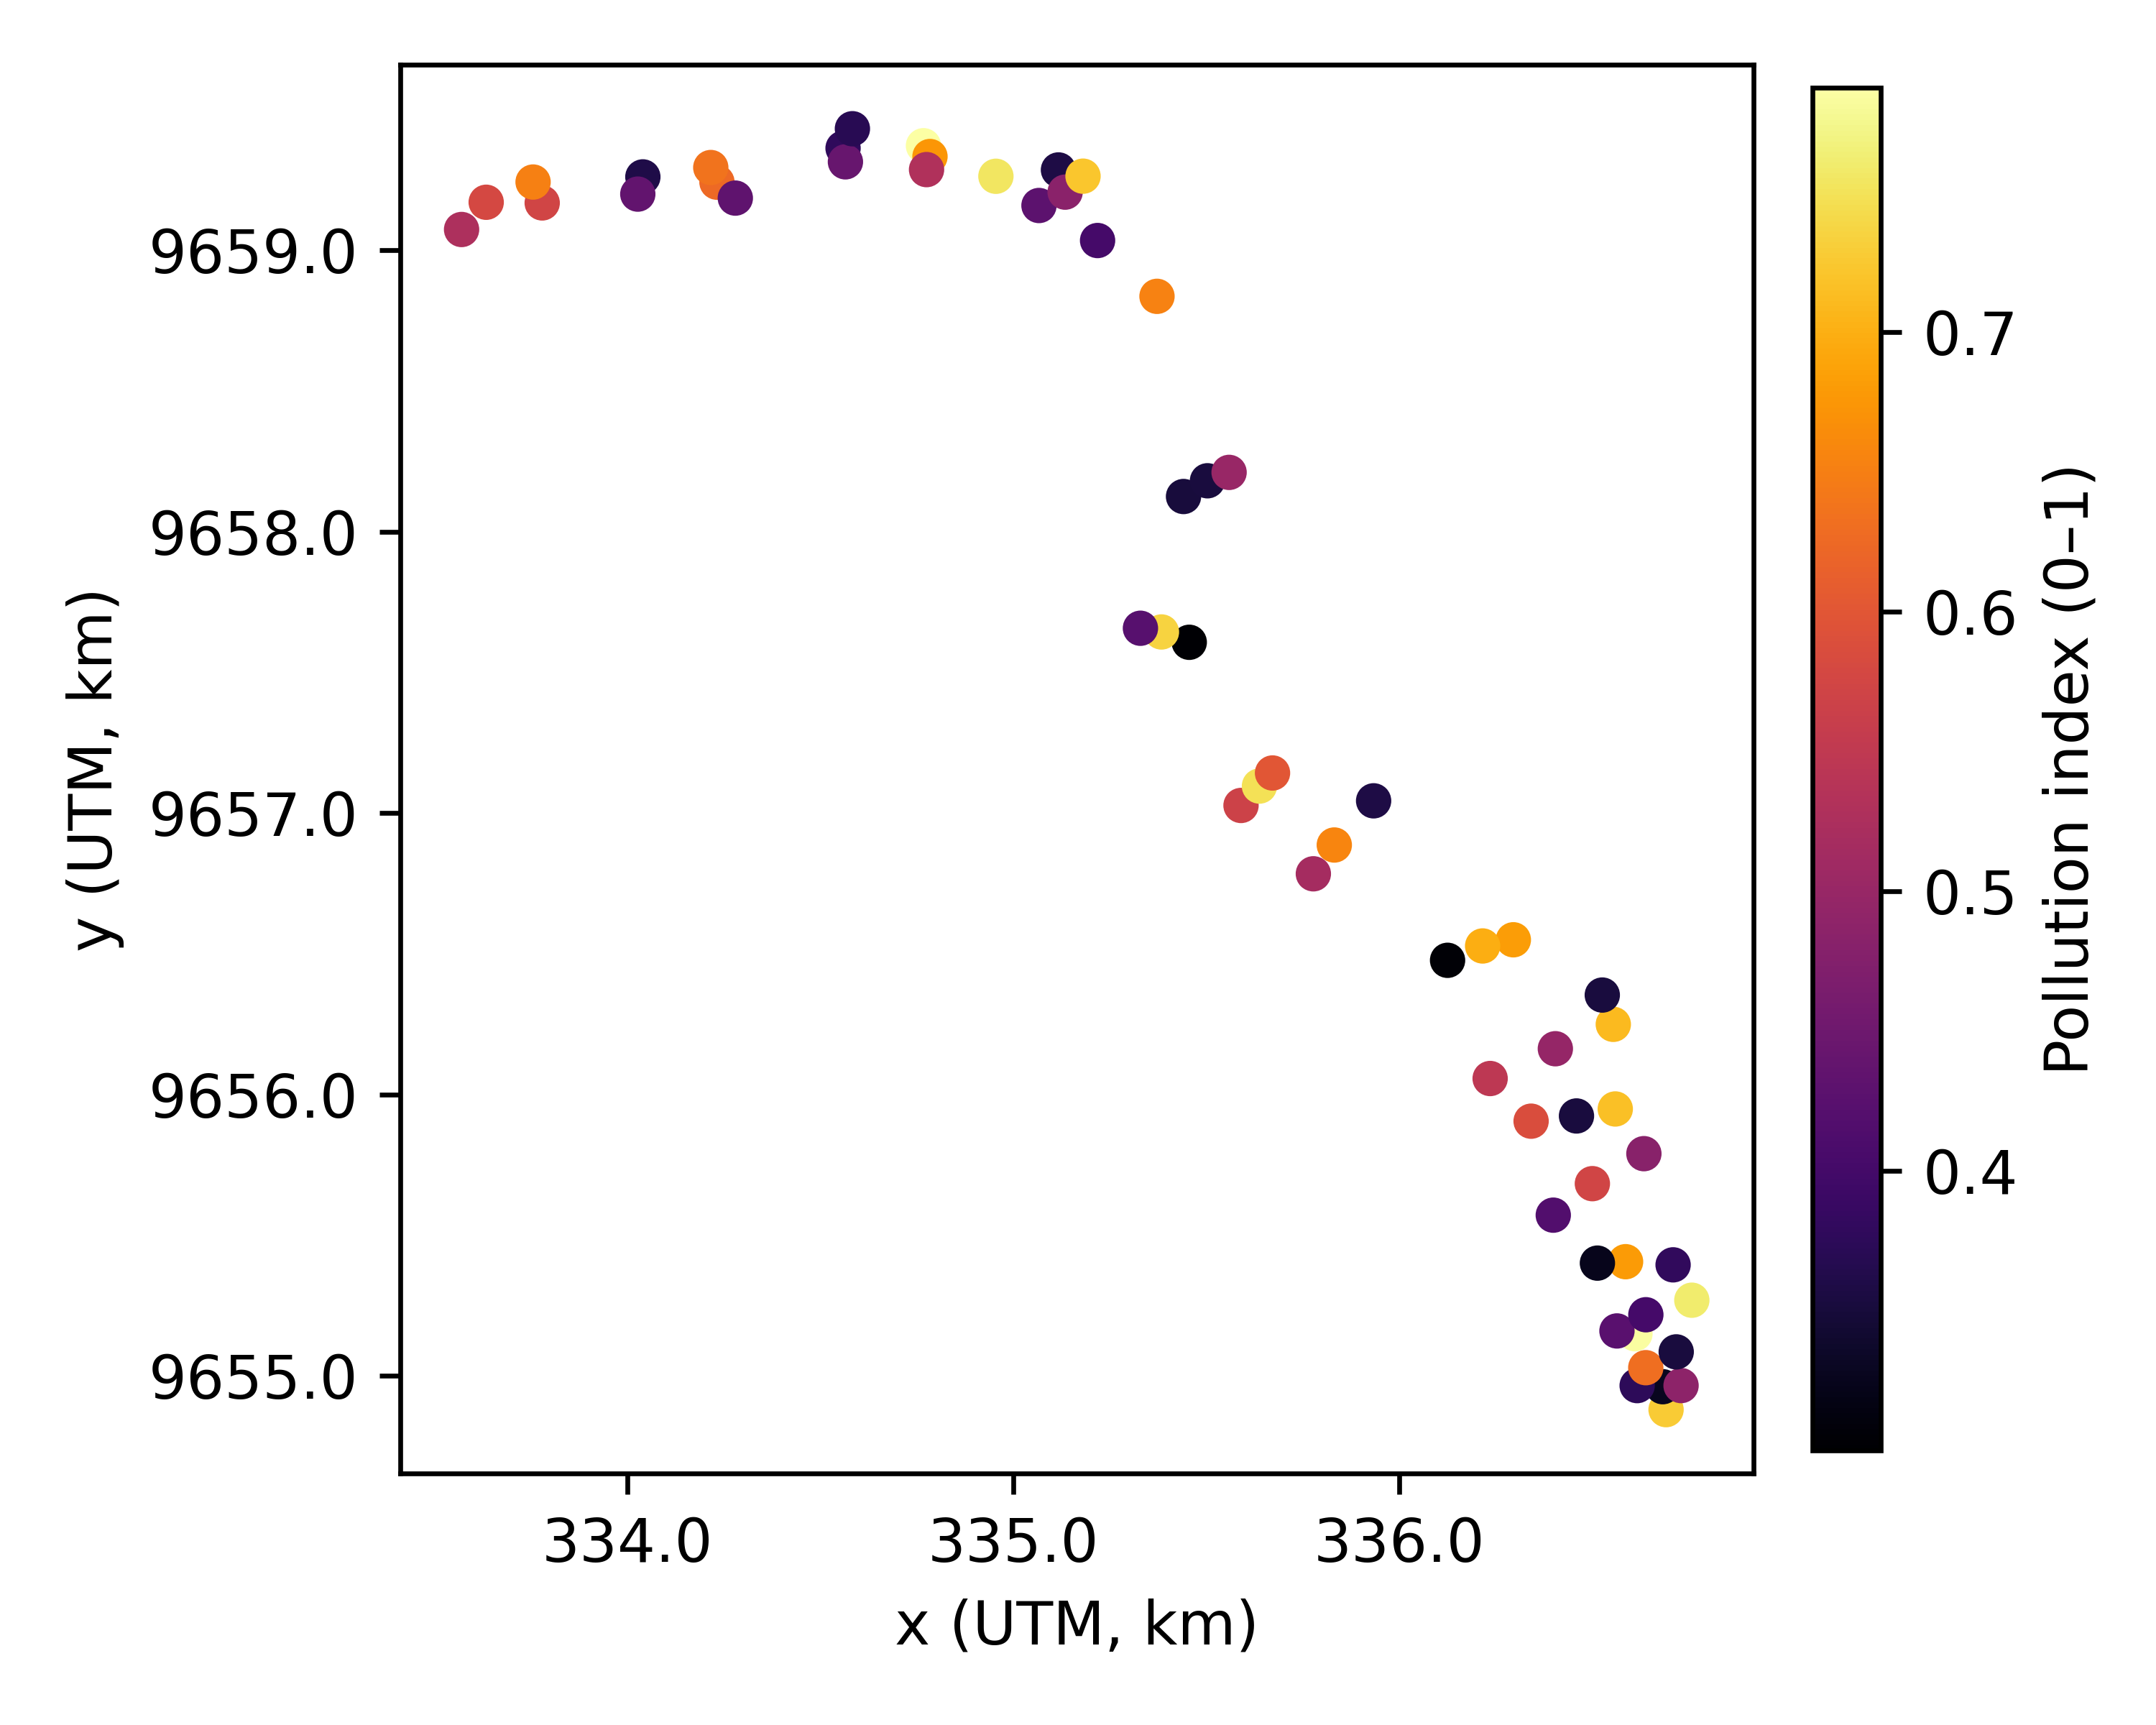
\includegraphics[width=\linewidth]{./figuras/pollution_scatter.png}
		\caption*{(a) Índice de poluição nos pontos}
	\end{minipage}\hfill
	\begin{minipage}{0.48\textwidth}
		\centering
		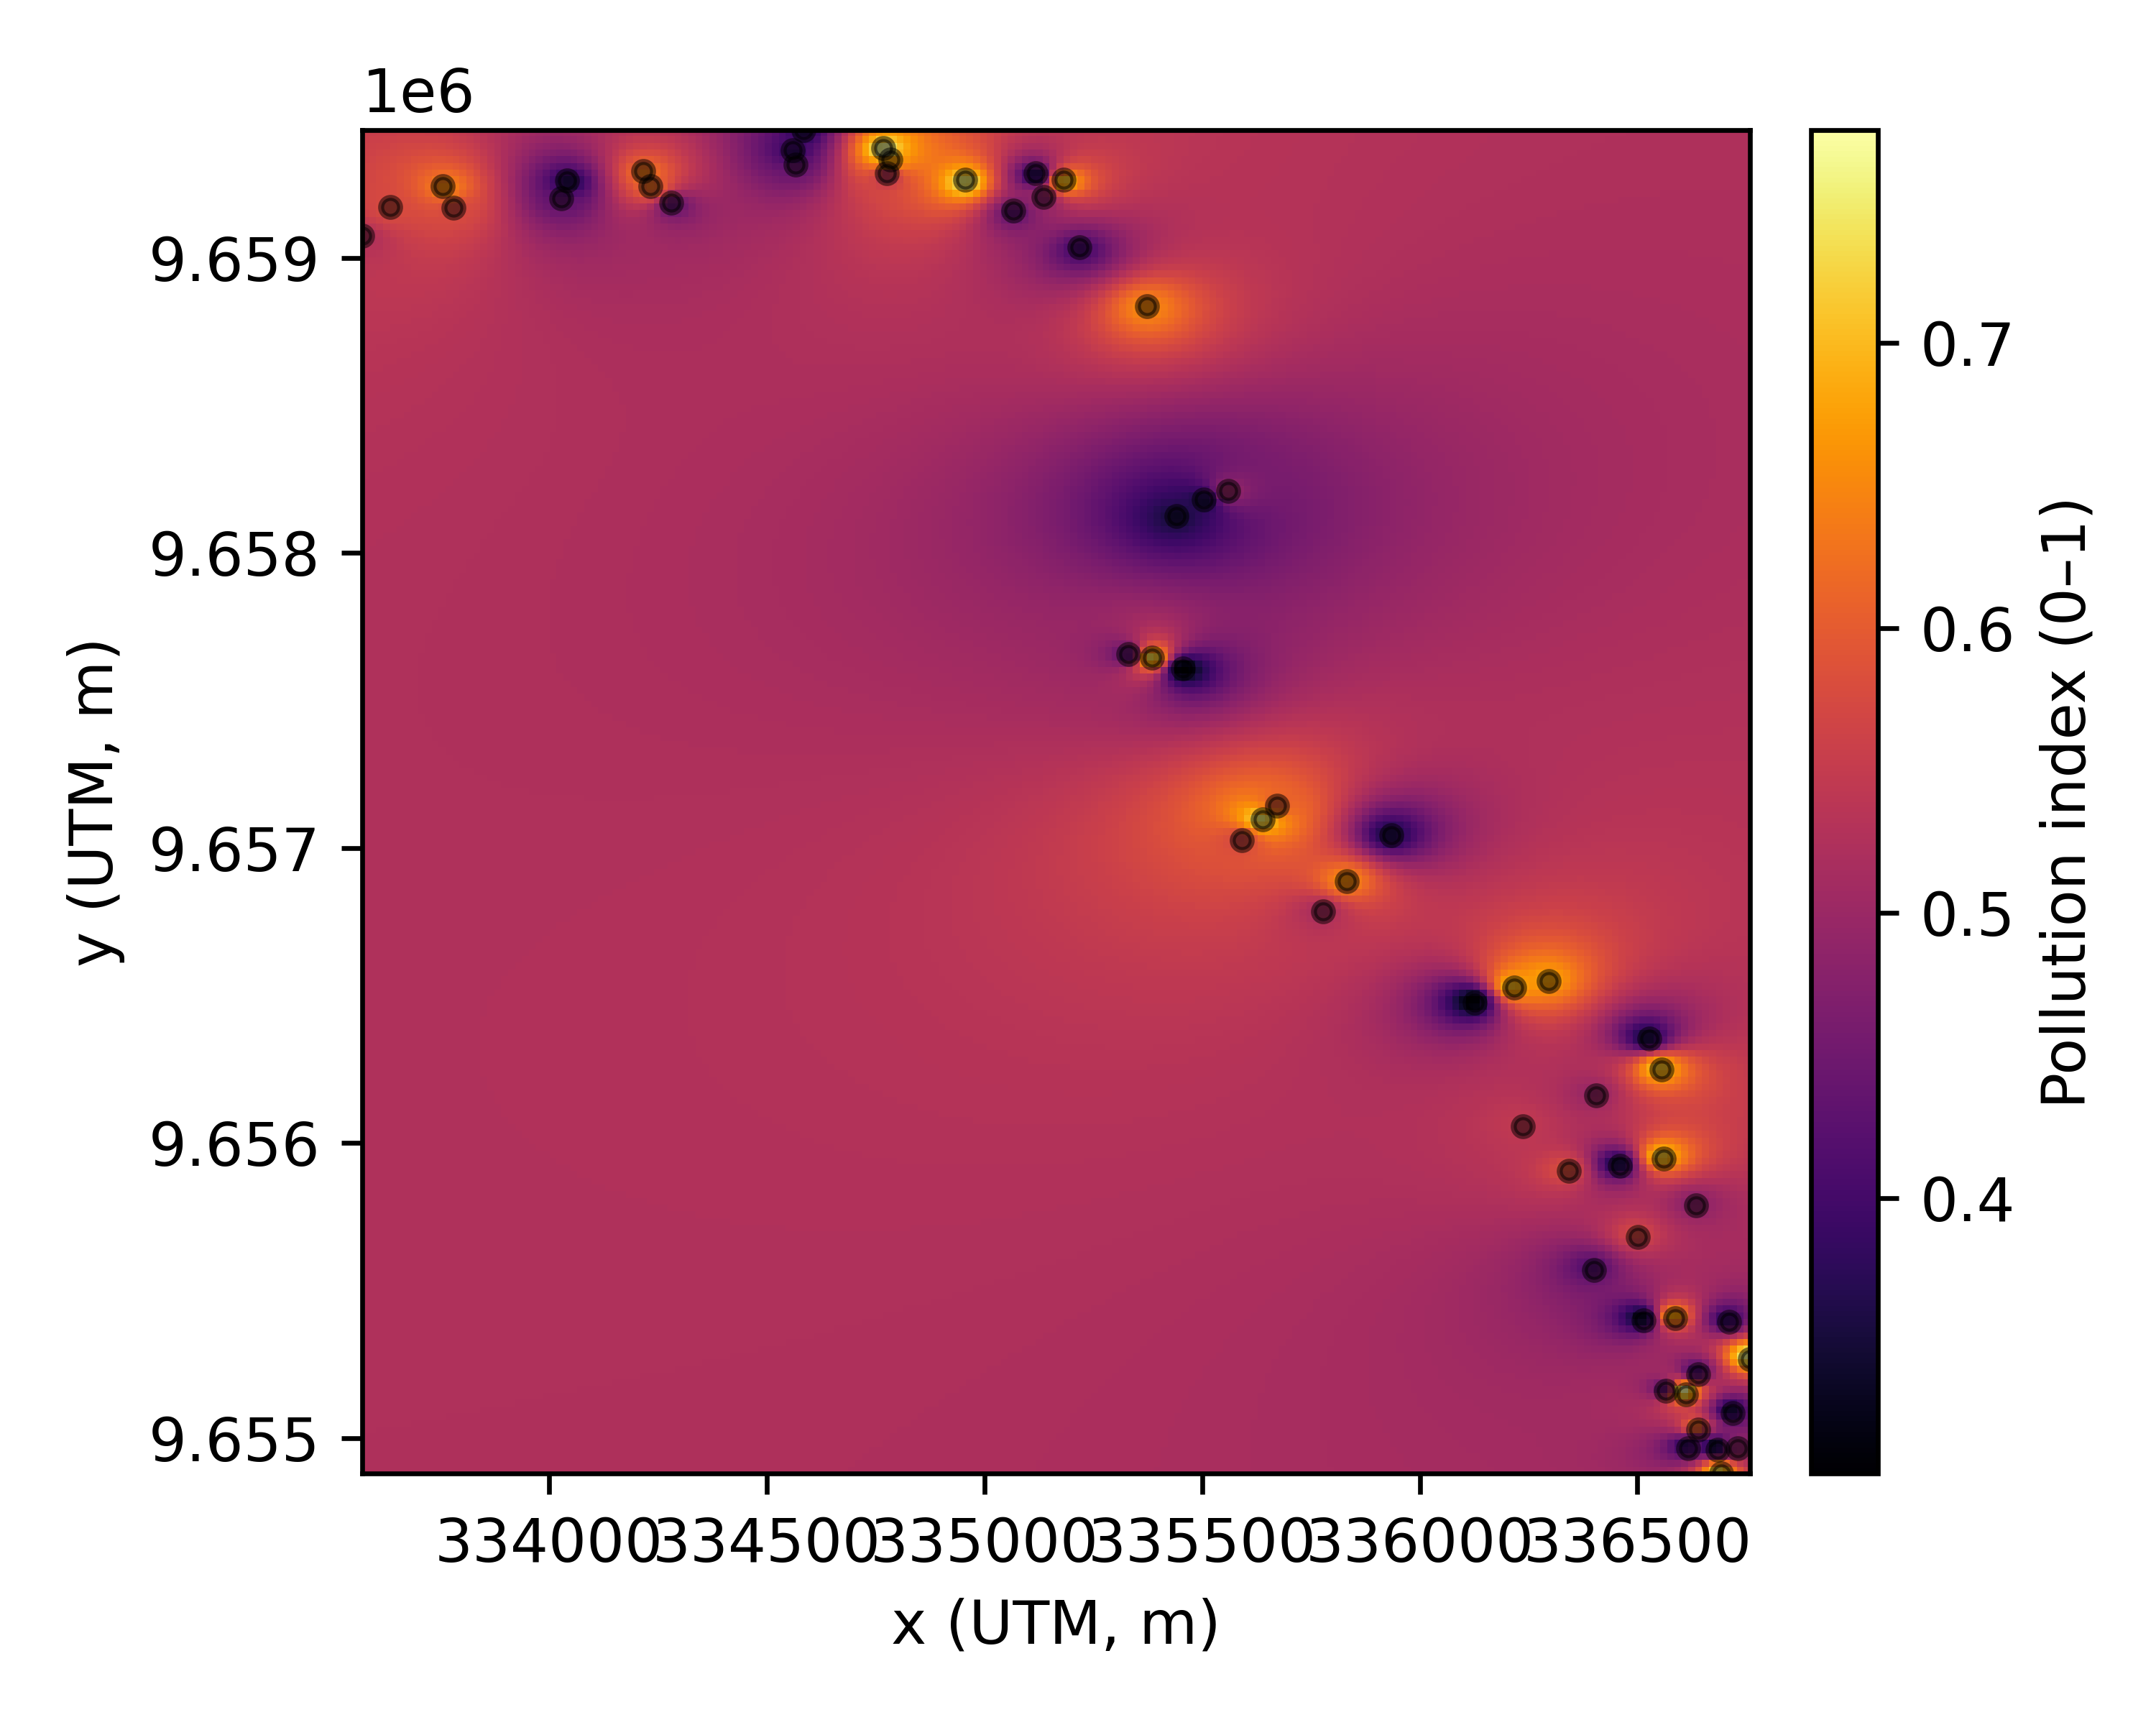
\includegraphics[width=\linewidth]{./figuras/pollution_idw.png}
		\caption*{(b) Mancha (IDW) do índice}
	\end{minipage}
	\caption{Estimativa espacial do índice de poluição composto a partir das
	predições multimodais.}
	\label{fig:pollution}
\end{figure}

A Figura~\ref{fig:pollution} apresenta o índice composto de poluição, combinando pH, OD e turbidez
em um único mapa. O gráfico de pontos evidencia locais com maior intensidade relativa, enquanto a
superfície interpolada por IDW permite visualizar a mancha de poluição estimada no corpo d’água.

\FloatBarrier

\section{DISCUSSÃO}

Os resultados indicam que a abordagem neuromórfica proposta é viável para predição de
parâmetros físico-químicos da água em ambiente amazônico, com desempenho consistente após
ajuste de hiperparâmetros e regularização por \textit{early stopping}. No cenário multimodal
sem vazamento de informação (sem uso das variáveis-alvo nas entradas), observou-se aumento da
dificuldade de predição, especialmente para turbidez, o que torna a avaliação mais realista
para uso em campo.

No benchmark com 10 sementes, Random Forest e LSTM apresentaram menores erros médios
globais, enquanto a SNN permaneceu competitiva e claramente superior ao MLP em robustez.
Os testes estatísticos reforçam essa leitura: não houve evidência de superioridade estatística
da SNN sobre Random Forest e LSTM para $\alpha=0{,}05$, mas houve vantagem significativa
da SNN sobre MLP. Portanto, os resultados sustentam a SNN como alternativa viável em
cenário de borda, ainda que não dominante em erro absoluto no conjunto atual.
Em termos espaciais, os mapas de pH, OD e turbidez revelam padrões coerentes de gradientes
e agrupamentos, o que reforça a consistência dos dados de campo e sugere que as variáveis
de entrada carregam informação relevante para a predição. As correlações entre temperatura,
cor aparente e turbidez observadas na análise exploratória estão alinhadas com processos
físico-químicos esperados em ambientes lênticos, fornecendo suporte adicional para o
modelo proposto.
Além do desempenho preditivo, a execução do modelo em Raspberry Pi 4B apresentou latência
sub-milissegundo por amostra, reforçando a viabilidade de inferência local em hardware de
baixo consumo e compatível com cenários remotos e offline.
\par
Do ponto de vista prático, a diferença entre modelos sugere que a escolha depende do objetivo
operacional. Random Forest e LSTM tendem a minimizar erro médio, enquanto a SNN oferece uma
alternativa robusta quando se prioriza inferência local com menor custo computacional e
potencial de eficiência energética. O comportamento mais instável do MLP confirma que modelos
densos clássicos são sensíveis em bases pequenas e podem variar de forma significativa entre
sementes. Além disso, a dificuldade sistemática na turbidez indica que esse parâmetro exige
informação adicional (por exemplo, variáveis hidrodinâmicas ou sazonais) para melhorar a
generalização.

\par
Outra consideração importante é que a codificação temporal por \textit{rate coding} implica
um compromisso entre fidelidade temporal e custo computacional: valores maiores de $T$ podem
aumentar a qualidade da representação, mas ampliam latência de inferência e consumo. Isso
sugere que, em cenários de uso real, a escolha de $T$ deve ser calibrada em função do contexto
operacional e das restrições energéticas do dispositivo de borda.

\section{CONCLUSÃO}

Este trabalho confirmou a viabilidade técnica da predição neuromórfica de qualidade
da água no Lago do Serpa, combinando modelagem multimodal, análise espacial e
implantação embarcada. Em nível de desempenho, a SNN apresentou resultados
competitivos e estáveis, superando o MLP no benchmark multissemente e mantendo
proximidade de desempenho com baselines clássicos. No conjunto avaliado, Random
Forest e LSTM apresentaram menor erro médio absoluto global, enquanto a SNN
permaneceu como alternativa robusta para inferência neuromórfica em borda.
Além disso, o ajuste de pesos da função de perda mostrou melhora específica em
turbidez com trade-off moderado no desempenho macro.

No eixo de aplicação, o modelo foi exportado para TensorFlow Lite e integrado em
aplicativo móvel offline, com inferência local de pH, OD e turbidez, cálculo de
índice de poluição e visualização geoespacial com mapa offline (MBTiles). Esse
resultado avança o trabalho além de uma prova de conceito puramente algorítmica,
demonstrando um fluxo completo de dados, treinamento, inferência embarcada e apoio
à decisão em campo.
No desenho neuromórfico, a adoção de \textit{rate coding} também se mostrou coerente
com o cenário de borda, pois permite ajustar explicitamente o equilíbrio entre qualidade
da representação temporal e latência de inferência no celular por meio do parâmetro $T$. Como limitações,
o estudo ainda depende de base amostral local e reduzida, o que restringe a generalização para outros
corpos hídricos e regimes sazonais; além disso, o aumento de dados sintético não substitui coletas reais,
e diferenças entre modelos podem variar com novas campanhas de campo. A validação prática foi feita em
Android, Raspberry Pi e ESP32, mas a extrapolação para outros microcontroladores e diferentes perfis de
energia requer medições adicionais e campanhas de campo mais amplas. Como continuidade desta pesquisa,
recomenda-se ampliar campanhas de coleta, validar o modelo em múltiplos cenários ambientais e medir de
forma sistemática latência, consumo energético e robustez operacional em diferentes dispositivos de borda.
Também é relevante evoluir a calibração do índice composto de poluição com apoio de especialistas
ambientais e testar estratégias de atualização de modelo em campo para diferentes regimes hidrológicos.

Como contribuição adicional, a validação em ESP32 mostrou que a inferência multimodal é viável
em microcontroladores, com latência de ordem de milissegundos e erros absolutos compatíveis com
o cenário móvel. A comparação energética entre ESP32, Raspberry Pi e smartphones evidenciou
trade-offs claros entre throughput e energia por inferência, reforçando a importância de escolher
plataforma e regime de amostragem conforme o contexto operacional.


%----------------------------------------------------------------------------------------
%   REFERÊNCIAS (via BibTeX / referencias.bib)
%----------------------------------------------------------------------------------------
\bibliographystyle{abntex2-alf}
\bibliography{referencias}

\end{document}
